% options:
% thesis=B bachelor's thesis
% thesis=M master's thesis
% czech thesis in Czech language
% english thesis in English language
% hidelinks remove colour boxes around hyperlinks

\documentclass[thesis=B,czech]{FITthesis}[2012/06/26]

\usepackage[utf8]{inputenc} % LaTeX source encoded as UTF-8

\usepackage{graphicx} %graphics files inclusion
\usepackage{float}
\usepackage{listings}
\usepackage[section]{placeins}
% \usepackage{amsmath} %advanced maths
% \usepackage{amssymb} %additional math symbols

\usepackage{dirtree} %directory tree visualisation

% % list of acronyms
% \usepackage[acronym,nonumberlist,toc,numberedsection=autolabel]{glossaries}
% \iflanguage{czech}{\renewcommand*{\acronymname}{Seznam pou{\v z}it{\' y}ch zkratek}}{}
% \makeglossaries

\newcommand{\tg}{\mathop{\mathrm{tg}}} %cesky tangens
\newcommand{\cotg}{\mathop{\mathrm{cotg}}} %cesky cotangens

% \usepackage[usenames,dvipsnames]{color}
% \usepackage{listings}
% \lstset{
%   columns=fullflexible,
%   language=Java,
%   numbers=left,
%   numbersep=5pt,
%   basicstyle=\small,
%   numberstyle=\footnotesize\color{Gray},
%   commentstyle=\it\footnotesize\color{Gray}
% }

% % % % % % % % % % % % % % % % % % % % % % % % % % % % % % 
% ODTUD DAL VSE ZMENTE
% % % % % % % % % % % % % % % % % % % % % % % % % % % % % % 

\department{Katedra softwarového inženýrství}
\title{Vývoj mobilních aplikací pomocí univerzálních platforem}
\authorGN{Štěpán} %(křestní) jméno (jména) autora
\authorFN{Heller} %příjmení autora
\authorWithDegrees{Štěpán Heller} %jméno autora včetně současných akademických titulů
\supervisor{Ing. Josef Gattermayer}
\acknowledgements{Mé poděkování patří zejména Bc. Dominikovi Veselému za cenné rady, které mi jako zkušený vývojář mobilních aplikací poskytl. Dále bych rád poděkoval všem, kdo mě v průběhu tvorby práce podporovali.}
\abstractCS{Práce zkoumá možnosti multiplatformního vývoje mobilních aplikací se zaměřením na frameworky, které umožňují vytvářet multiplatformní aplikace pomocí webových technologií. Práce poskytuje srovnání jednotlivých frameworků, technologický popis tohoto přístupu a také detailní analýzu frameworku PhoneGap, který je pionýrem v této kategorii. Cílem práce je poskytnout srovnání mezi vývojem nativní cestou a vývojem pomocí frameworků jako je právě PhoneGap.}
\abstractEN{This thesis explores the options of mobile application cross-platform development with a special focus on those frameworks which enable to develop these applications using web technologies. The thesis provides a comparison of individual frameworks, a technological description of this approach and also a detailed analysis of a leader in this field – the PhoneGap framework. The ultimate goal of this thesis is to provide a comparison between developing applications in the native way and developing them via frameworks like PhoneGap.}
\placeForDeclarationOfAuthenticity{V~Praze}
\declarationOfAuthenticityOption{1} %volba Prohlášení
\keywordsCS{mobilní aplikace, hybridní aplikace, multiplatformní vývoj, PhoneGap, hybridní framework, webové technologie, iOS, Android, Windows Phone}
\keywordsEN{mobile application, hybrid application, mobile app, hybrid app, cross-platform development, PhoneGap, hybrid framework, web technologies, iOS, Andorid, Windows Phone\clearpage}
%\setcounter{tocdepth}{5}

\begin{document}

% \newacronym{CVUT}{{\v C}VUT}{{\v C}esk{\' e} vysok{\' e} u{\v c}en{\' i} technick{\' e} v Praze}
% \newacronym{FIT}{FIT}{Fakulta informa{\v c}n{\' i}ch technologi{\' i}}

\begin{introduction}
	%sem napište úvod Vaší práce
\end{introduction}

% Kapitola Mobilní zařízení a aplikace
\chapter{Mobilní zařízení a aplikace}
	\section{Smartphone}
Smartphone (česky „chytrý telefon“) v sobě kombinuje funkce mobilního telefonu a klasického počítače. Od klasických mobilních telefonů (tzv. „feature phone“) se smartphone liší v několika věcech:

\begin{enumerate}
	\item Přítomností pokročilého operačního systému (iOS, Android, Windows Phone/Mobile apod.)
	\item Přítomností lokálního úložiště, které může uživatel použít pro uložení vlastních dat.
	\item Možností připojit se telefonem k internetu a stahovat z něj data.
\end{enumerate}

Společnost Gartner definuje smartphone jako zařízení, které používá jasně rozpoznatelný operační systém umožňující vývojářům třetích stran vyvíjet pro tento systém aplikace (více o tom jak definujeme aplikace nastíní podkapitola \ref{Sec:Aplikace}). Aplikace třetích stran je možné instalovat a odstraňovat a při jejich vývoji je použito API daného operačního systému. Operační systém zajišťující fungování smartphone musí podporovat možnost používat více aplikací současně (tzv. multitasking) \cite{gartner_smartphone_definition}. 

Výrobci moderních smartphonů vybavili tento přístroj mnoha dalšími funkcemi. Mezi ty rozšířené patří například:

\begin{enumerate}
	\item fotoaparát/digitální kamera
	\item dotyková obrazovka s vysokým rozlišením
	\item možnost zaznamenávat zvuk
	\item GPS navigace
	\item přehrávač multimédií atd.
\end{enumerate}

\subsection{Rozšíření smartphonů}
První zařízení, které můžeme označit pojmem smartphone (i když samotný termín ještě vymyšlen nebyl), bylo uvedeno na trh v roce 1994 pod označením „Simon Personal Communicator“, za jehož vývojem stála firma IBM \cite{simon}. Nabízel černobílý dotykový displej, který umožňoval ovládání přístroje prstem či stylusem a poskytoval uživatelům aplikace jako e-mailový klient, kalendář, hodiny a jednoduché hry. Vůbec poprvé termín „smartphone“ použila firma Ericsson při uvedení svého nového modelu GS88 s kódovým označením „Pandora“ \cite{history_of_the_smartphone}.

Mezi širokou veřejností je však za první smartphone považován až iPhone společnosti Apple, jehož první verze byla uvedena do prodeje v roce 2007 \cite{apple_unveils_iPhone}. Od momentu, kdy byl iPhone uveden na trh, zaznamenává podíl prodaných smartphonů ke klasickým telefonům (feature phone) dynamický růst. V roce 2011 tvořily, dle odhadů společnosti Ericsson, 30 \% prodaných mobilních telefonů smartphony, což činí oproti roku 2010 nárůst o 10 \% \cite{ericsson_report_web}. Celkový podíl používaných smartphonů ke klasickým telefonům je pak odhadován na 10 \%, tedy asi 1 miliarda zařízení \cite{ericsson_report_web}.

\subsection{Významní výrobci}
Od uvedení prvních smartphonů na trh v druhé polovině devadesátých let vládla tomuto segmentu jednoznačně Nokia. Toto zaběhnuté paradigma se začalo pozvolna měnit až s příchodem iPhonu. Na grafu \ref{fig:VyrobciSmartphoneRozsireni}, který mapuje období mezi léty 2009–2012 je jasně vidět strmý pád Nokie a naopak vzestup konkurentů v podobě Applu, Samsungu a dalších.

\begin{figure}\centering
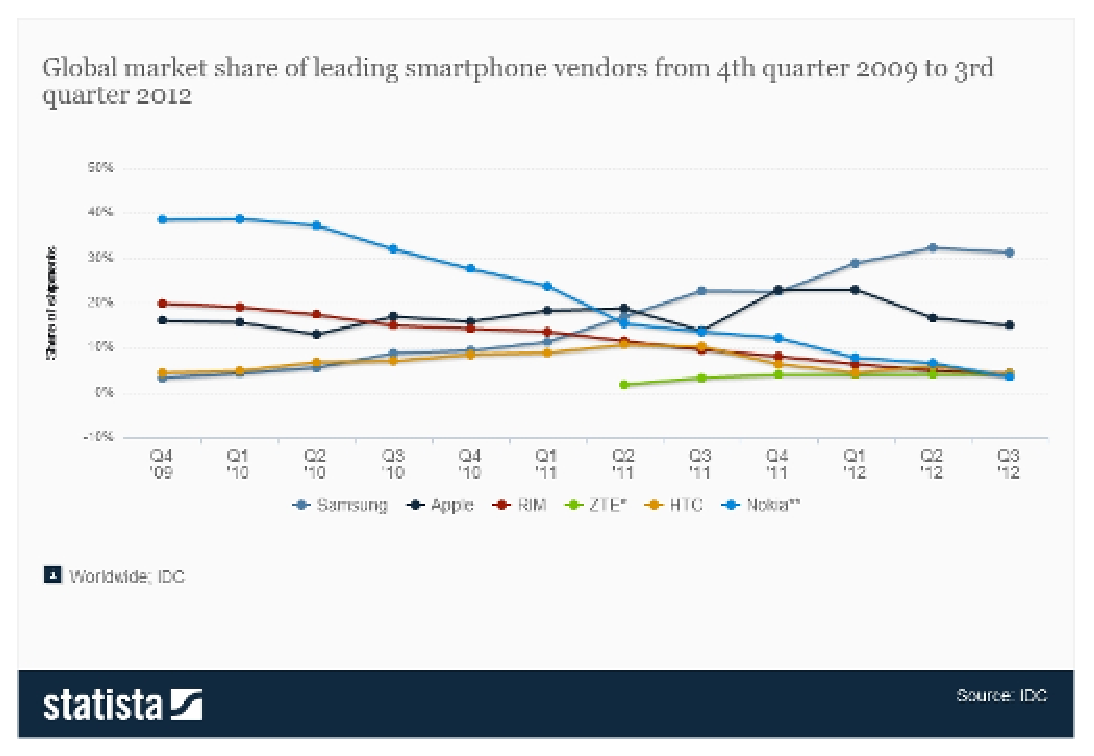
\includegraphics[width=1.0\textwidth]{smartphone_marketshare_vendors.eps}
\caption{Vývoj tržního podílu výrobců chytrých telefonů}
\label{fig:VyrobciSmartphoneRozsireni}
\end{figure}

Aktuální data z června roku 2012 ukazují zřetelnou převahu společnosti Samsung nad zbytkem trhu. Více než třetina dnes používaných smartphonů nese značku právě této společnosti. Oproti tomu zhruba polovičním podílem na trhu se může pochlubit společnost Apple. Původní hegemon – firma Nokia – nyní okupuje pouze lehce přes 6 \% tržního podílu.

\begin{figure}\centering
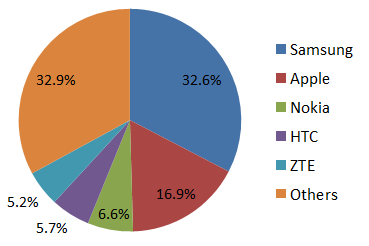
\includegraphics[width=0.6\textwidth]{smartphone_by_manufaturers.png}
\caption{Současný tržní podíl výrobců smartphonů na trhu}
\label{fig:VyrobciSmartphoneRozsireni2}
\end{figure}

\section{Přehled mobilních platforem}
Řada zákazníků při výběru nového chytrého telefonu dbá nejen na vzhled a hardwarové parametry, ale důležitou roli při konečném rozhodování hraje i operační systém, který na přístroji běží. Někteří výrobci se snaží s konkrétním operačním systémem spojit svou značku (Apple, Nokia), jiní naopak dávají zákazníkům na výběr různé modely s různými systémy (HTC, Samsung).

\subsection{iOS}
iOS je produktem společnosti Apple, která jím vybavuje své produkty iPhone, iPod i iPad. Poprvé byl uveden v roce 2007 spolu se smartphonem iPhone na konferenci Macworld \cite{apple_unveils_iPhone}. Od té doby je neustále vylepšován a v současné době se již nachází ve verzi 6. Od dob první verze se však uživatelské prostředí iPhonu mění jen pozvolna. Apple, narozdíl od konkurence v podobě Androidu a Windows Phone, neumožňuje použití systému iOS na zařízeních, které nevyrobila firma Apple.

Celý koncept systému iOS je úzce spjat s velkým displejem smartphonu iPhone. Ovládání celého prostředí je uživateli umožněno pomocí celé řady multi-dotykových gest. Mezi nejznámější prvky z prostředí systému iOS můžeme zařadit tzv. „Home screen“, který pomocí matice ikon usnadňuje uživateli spouštění nainstalovaných aplikací. Dále stojí za zmínku například notifikační centrum, hlasové ovládání Siri nebo Game center.

\subsubsection{Vývojářské technologie}
Aplikace pro systém iOS se programují primárně v jazyce Objective-C \cite{introduction_ios_development}. Objective-C je objektově orientovaný, reflektivní jazyk, v němž lze nalézt společné rysy se známým jazykem SmallTalk \cite{bp_dominik}. Poměrně složitá syntaxe Objective-C představuje značnou překážku pro začínající vývojáře, protože se výrazně liší od ostatních běžně používaných jazyků (například Javy v Androidu).

Díky kompilační struktuře naznačené v předchozí kapitole můžeme však místo Objective-C použít alternativní programovací jazyky, pokud k nim najdeme vhodný front-end. Toho využívá například projekt Monotouch, který vám umožňuje programovat nativní aplikace v C\# a frameworku .NET \cite{xamarin_monotouch}.

\subsubsection{Vývojářské nástroje}
Apple dává vývojářům k dispozici balík iOS SDK, který obsahuje široké spektrum nástrojů potřebných k tvorbě nativních aplikací pro systém iOS. Tento balík obsahuje například vývojové prostředí XCode, emulátor pro simulovaný běh aplikací na virtuálním zařízení, nástroj pro designování grafických prvků navrhované aplikace, offline verzi dokumentace a mnoho dalšího.

Pro vývoj aplikací pro iOS je nutné vlastnit počítač s operačním systémem Mac OS X. Toto je další poměrně značná překážka pro začínající vývojáře neboť počítače s tímto systémem jsou prozatím na trhu zastoupeny v marginální míře a konkurence v podobě Androidu umožňuje vyvíjet aplikace pro tento systém na libovolné platformě.  Pro publikování aplikací v tržišti App Store je navíc potřeba vlastnit placený vývojářský účet \cite{distribute_ios_app}.

\subsection{Android}
Operační systém Android byl původně vytvořen společností Android Inc., kterou v roce 2005 odkoupil gigant v oblasti internetového vyhledávání – firma Google \cite{google_buys_android}. Představení Androidu veřejnosti bylo úzce spjato se založením organizace Open Handset Alliance, která sdružovala výrobce software, hardware i telefonní operátory s cílem vyvinout otevřenou platformu a definovat nové standardy na poli mobilních telefonů \cite{android_announce}. Systém Android je šířen pod licencí Apache License a lze jej tedy označit za open-source software \cite{android_overview}.

Systém Android můžeme krom mobilních telefonů nalézt i na tabletech, chytrých televizích, herních konzolích a dalších zařízeních. Vysoká obliba Androidu mezi zákazníky pramení především z obrovského množství různých modelů, se kterými je tento systém na trhu nabízen. Vzhledem k otevřené licenci, pod kterou je systém šířen, je využíván širokým portfoliem výrobců, kteří tak ušetří za vývoj a správu vlastního systému.

Uživatelské rozhraní Androidu vzdáleně připomíná svého konkurenta iOS. Také zde najdeme „Home screen“, který je tvořen maticí ikon symbolizujících nainstalované aplikace. Stejně tak v Androidu můžeme nalézt třeba notifikační centrum. Od svých konkurentů se tato platforma odlišuje nepřeberným množstvím možností, jak upravit vzhled a chování systému.

\subsubsection{Vývojářské technologie}
Pro vývoj nativních aplikací se používá programovací jazyk Java. Podle společnosti TIOBE se jedná o druhý nejpoužívanější programovací jazyk na světě \cite{tiobe_software}. Java je objektově orientovaný jazyk se syntaxí blízkou jazykům C a C++.

Velkou výhodou Javy je její platformní nezávislost. Vlastní kód se totiž překládá do tzv. mezikódu, který je poté interpretován v rámci Java Virtual Machine \cite{understanding_jvm_internals}. Program napsaný v Javě je tak spustitelný na Windows, Mac OS X i Linuxu.

\subsubsection{Vývojářské nástroje}
Google, podobně jako Apple, připravil pro externí vývojáře balík všeho potřebného pro vývoj nativních aplikací, tzv. Android SDK. Ten obsahuje velmi populární vývojové prostředí Eclipse IDE obohacené o plugin ADT (Android Developer Tools). Toto rozšíření se stará o hlubokou integraci nástrojů samotného SDK do vývojového prostředí. Poskytuje tak GUI přístup například k debugovacím nástrojům (DDMS), návrhovým nástrojům pro uživatelské rozhraní, přístup a konfiguraci emulátorů a podobně.

Součástí SDK jsou samozřejmě i zdrojové kódy nejnovější verze systému Android a také obraz systému spustitelný v emulátoru. Nechybí ani podrobná dokumentace pro offline použití.

\subsection{Windows Phone}
Windows Phone vznikl ve společnosti Microsoft jako odpověď na úspěch iOS a Androidu. Předešlý systém z dílmy redmondské firmy, Windows Mobile, již nebyl lákavý pro výrobce zařízení s velkými dotykovými obrazovkami. Microsoft tak představil počátkem roku 2010 na Mobile World Congress v Barceloně zcela nový operační systém, který nesl označení Windows Phone 7 \cite{ms_announce_wp}. Jeho uživatelské rozhraní tvořené velkými barevnými interaktivními dlaždicemi se na první pohled velmi liší od iOS a Androidu, avšak většinu principů práce s dotykovými zařízeními zachovává. 

Společnost Microsoft narozdíl od Applu či Google doposud nevyrábí vlastní chytré telefony a tak přijetí nové platformy bylo čistě na vůli výrobců telefonů. Na tomto poli se nový systém střetával především s Androidem, který je výrobcům k dispozici zdarma, zatímco Microsoft požaduje za použití Windows Phone licenční poplatky. Jako svůj hlavní systém si Windows Phone zvolila společnost Nokia, která se spolu s ním snaží dobýt zpět své ztracené pozice na trhu s chytrými telefony.

Od roku 2010, kdy byl systém poprvé představen, byl již několikrát vylepšen mnoha aktualizacemi, které přinášely do systému nové funkce (např. multitasking). Dva roky po uvedení systému Windows Phone Microsoft oznámil vydání nové verze svého systému pod názvem Windows Phone 8, která přináší přepracované jádro a některé nové funkce \cite{ms_unveils_wp8}.

\subsubsection{Vývojářské technologie}
Pro vývoj aplikací pro systém Windows Phone 8 (ale i pro desktopové Windows) se primárně používá jazyk C\#. Tento jazyk byl vyvinutý spolu s frameworkem .NET firmou Microsoft. C\# je objektově orientovaný jazyk, u jehož syntaxe se Microsoft inspiroval u programovacích jazyků z rodiny C. Některé aspekty však přejal také z oblíbené Javy.

Framework .NET je komplexní balík knihoven a rozhraní určených pro vývoj, kompilaci a spouštění aplikací pro platformu Windows.

\subsubsection{Vývojářské nástroje}
Také pro platformu Windows Phone 8 existuje balík nástrojů určený pro vývoj nativních aplikací – Windows Phone 8 SDK. Jeho součástí je odlehčená verze Microsoft Visual Studia – Visual Studio Express 2012. Visual Studio je velmi oblíbené vývojové prostředí s širokým spektrem funkcí, jež sou vývojářům k dispozici. SDK obsahuje množství nástrojů pro návrh, testování, debugování a emulátory pro běh uživatelských aplikací.

\subsection{Firefox OS}
Firefox OS je mobilní operační systém, který je v současné době stále ještě ve vývoji a neběží tedy zatím na žádném reálně používaném zařízení. V této práci jej zmiňuji proto, že cíle, které si společnost Mozilla, jež stojí za tímto systémem, vytyčila, přímo korespondují s tématem této práce (více technických podrobností o Firefox OS naleznete v kapitole 2).

Vývoj systému Firefox OS byl oznámen v červnu 2011 v rámci komunity společnosti Mozilla. Celý projekt nesl kódové označení „Boot to Gecko“ a jeho cílem má být položení rovnítka mezi webové technologie a moderní mobilní telefony. V originální oznamovací zprávě se přímo říká \cite{booting_to_the_web}: „Chceme identifikovat překážky, které stěžují webovým vývojářům tvorbu aplikací, které budou v každém směru plnohodnotnými náhradami nativních aplikací pro platformy iOS, Android a WP7.“ První telefony s Firefox OS by se měly objevovat v prvním čtvrtletí roku 2013 \cite{ztes_first_firefoxos}.

\subsubsection{Aplikační technologie}
Protože nativní aplikace pro systém Firefox OS není nic jiného než „trochu vylepšená“ webová stránka (přesněji tzv. Open Web App \cite{faqs_mozilla}), nemůžeme od Firefox OS očekávat jakýkoliv proces kompilace.

Taková webová aplikace může samozřejmě fungovat jako běžná webová stránka uvnitř internetového prohlížeče. Uživatelé ovšem obvykle očekávají od mobilní aplikace více než od webové stránky. Aplikace ve Firefox OS běží mimo internetový prohlížeč. Ke svému běhu využívají tzv. Web runtime. Web runtime je software obsažený v internetovém prohlížeči, který však může běžet samostatně a zajišťuje celý životní cyklus aplikace od jejího spuštění, po obsluhu jejích požadavků až po její ukončení uživatelem \cite{apps_architecture}.

\subsubsection{Vývojářské technologie}
Jelikož jsme již naznačili, že pro vývoj nativních aplikací pro Firefox OS se používají pouze webové technologie dnes souhrnně (nesprávně?) označované jako rodina HTML5, do kterých řadíme:

\begin{enumerate}
	\item HTML5 jako značkovací jazyk ve své páté (dosud neoficiální) verzi obohacen o mnohé moderní funkce jako je geolokace, lokální databáze či nativní podpora pro přehrávání videa a audia.
	\item CSS3 pro definici vzhledu a částečně i chování uživatelského rozhraní aplikace.
	\item JavaScript je interpretovaný programovací jazyk, který se používá pro zajištění aplikační logiky. Jeho syntaxe se inspirovala u programovacích jazyků C/C++ a Java.
\end{enumerate}

\subsection{Vývojářské nástroje}
Mozilla nenabízí vývojářům aplikací pro Firefox OS (který stále ještě není v oficiálním prodeji) žádný balík se vším potřebným jako je tomu u jiných platforem. Důvodem pro tento fakt je pravděpodobně všudypřítomnost vývojářských nástrojů pro webové stránky/aplikace.

Přesto však firma Mozilla na konci roku 2012 vydala emulátor systému Firefox OS, na kterém mohou vývojáři testovat své aplikace aniž by museli vlastnit reálné zařízení. Firefox OS Simulator existuje pro Windows, Mac i Linux a lze jej dokonce získat i jako plugin do desktopové verze internetového prohlížeče Firefox \cite{announcing_fxOS_simulator}.

\subsection{Situace na trhu}
Podíváme-li se na aktuální situaci na trhu, můžeme jasně vidět, že na tomto poli nyní zcela zřetelně dominuje systém Android. Naopak dřívější hegemon Symbian, který poháněl zařízení společnosti Nokia, má již méně než 5 \% tržního podílu. iOS od Applu je pak druhým největším hráčem.

\begin{figure}\centering
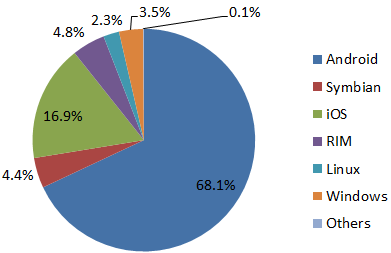
\includegraphics[width=0.6\textwidth]{smartphone_by_platform.png}
\caption{Současný tržní podíl mobilních platforem}
\label{fig:MobilniPlatformyPodil}
\end{figure}

Další graf\ref{fig:MobilniPlatformyVyvoj} jasně ilustruje již zmíněné trendy. Můžeme zde vidět strmý propad Symbianu a naopak drtivý vzestup platformy Android, který od roku 2009 zaznamenala. 

\begin{figure}\centering
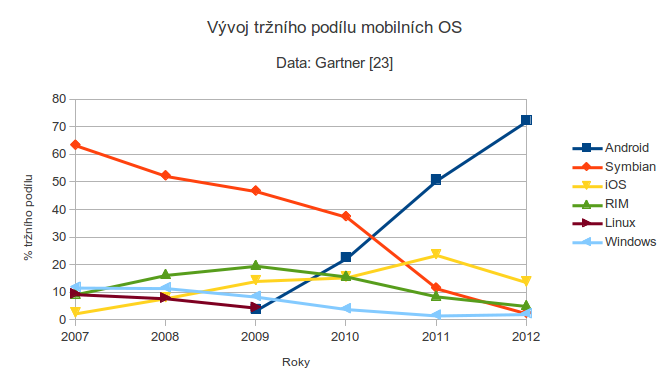
\includegraphics[width=1.0\textwidth]{graf_vyvoj_mobilnich_os.png}
\caption{Vývoj tržního podílu mobilních platforem}
\label{fig:MobilniPlatformyVyvoj}
\end{figure}

\section{Mobilní aplikace} \label{Sec:Aplikace}
Mobilní aplikaci definujeme jako samostatný software určený pro využití na smartphonech, tabletech a dalších přenosných zařízeních. Zpravidla jsou velmi úzce zaměřené na vykonání konkrétní činnosti a mají velmi málo funkcí (např. kalkulačka, internetový prohlížeč, čtečka RSS apod.).

Mobilní aplikace jsou převážně distribuovány přes takzvaná „tržiště“, kde uživatel najde kategorizovaný přehled aplikací, které si může pro svou platformu stáhnout (více o tržištích v podkapitole XY). Některé platformy podporují i možnost stahování mobilních aplikací prakticky odkudkoliv, například z webových stránek vývojáře, který aplikaci vytvořil (Android).

\subsection{Rozdělení mobilních aplikací}
Pro rozdělení mobilních aplikací můžeme využít v zásadě dva přístupy. Jedním z nich je rozdělit aplikace podle účelu, za nímž byly stvořeny. Další možností je potom rozdělit takové aplikace dle technologie, pomocí které byly vytvořeny.

\subsubsection{Rozdělení dle účelu}
Při rozdělování aplikací dle účelu se musíme zaměřit na oblast činnosti, kterou má daná aplikace svému uživateli zpříjemnit. Níže jsem provedl jejich rozdělení dle účelu, při jehož tvorbě jsem vycházel z kategorizace, kterou pro rozdělení aplikací používají oficiální tržiště pro platformy iOS a Android.

\begin{enumerate}
	\item Hry
	\item Sociální sítě
	\item Multimédia – například aplikace na úpravu fotografií, přehrávání videa nebo hudby.
	\item Produktivita – GTD aplikace, time tracking apod.
	\item Komunikace – IM komunikátory, SMS aplikace apod.
	\item Doprava – GPS navigace, mapy apod.
	\item Cestování
	\item Kancelářské – zjednodušené verze kancelářských balíků, správa financí apod.
	\item Zábava
	\item. Nakupování – tipy, slevy apod.
	\item Informační – čtení zpráv, vzdělávání, počasí.
	\item Úpravy systému – rozšířené možnosti nastavení a úprav vzhledu.
	\item Životní styl – zdraví, jídlo.
	\item Sport – živé výsledky, informace.
\end{enumerate}

\subsection{Dle technologie}
\subsubsection{Nativní aplikace}
Již ze slova „nativní“ v názvu této sekce plyne, že půjde o technologii, která je nějakým způsobem přirozená. V našem případě je to přirozenost technologie a chování aplikace k dané platformě. Pro vývoj mobilní aplikace pro konkrétní operační systém tedy používáme určitý programovací jazyk a určité nástroje. 

Nativní aplikace se většinou vyznačují dobrým výkonem a širokým spektrem funkcí. Vývojáři nativních aplikací mají totiž přístup k drtivé většině hardwarových i softwarových funkcí telefonu. I vzhled nativních aplikací je přesně takový, jaký ho uživatel očekává. Některé platformy mají totiž velmi striktní požadavky na vzhled jednotlivých ovládacích prvků (tlačítek, přechodů apod.) a nevyhovující aplikace vůbec nepřipouští na svá tržiště.

Nativní aplikace jsou většinou distribuovány přes oficiální tržiště konkrétní platformy. U operačního systému Android však můžeme pozorovat i jiné cesty, kterými uživatelé aplikace získávají (z webových stránek, neoficiální tržiště apod.). Více o vývoji nativních aplikací pro jednotlivé platformy si řekneme v kapitole 2.

\subsubsection{Webová aplikace}
Aplikaci označujeme jako webovou, pokud bylo při jejím vývoji použito tzv. webových technologií (např. HTML či JavaScript). Webová aplikace ke svému běhu potřebuje internetový prohlížeč nebo jeho jádro. Všeobecná rozšířenost webových aplikací pramení právě z tohoto faktu. Internetový prohlížeč je totiž předinstalován na všech známých operačních systémech (desktopových i mobilních) a díky tomu je velmi široce rozšířený.

V prostředí mobilních telefonů nacházejí webové aplikace uplatnění zejména díky nízkým nákladům na vytvoření a jejich multiplatformnosti. Webová aplikace na mobilním telefonu může mít buď formu webové stránky uzpůsobené pro zobrazení na malých displejích či offline aplikace, která ke svému běhu nevyžaduje internetové připojení.

Velkým nedostatkem, jímž webové aplikace trpí, je jich omezená funkcionalita. Webové aplikace nemohou přistupovat k žádným specifickým funkcím telefonu vyjma samotného internetového prohlížeče. Proto se webové aplikace využívají především jako zobrazovač obsahu, který je formátován pro snadnou konzumaci na mobilním telefonu.

\subsubsection{Hybridní aplikace}
Definice hybridních aplikací není zatím úplně přesně vymezená. Pokud bych se měl pokusit takovou aplikaci definovat, tak se jedná o aplikaci, pro jejíž vývoj bylo použito převážně webových technologií, avšak hybridní aplikace umožňuje uživateli využívat některé hardwarové i softwarové funkce telefonu stejně, jako by se jednalo o aplikaci nativní.

Hybridní aplikace se navenek tváří stejně jako aplikace nativní, takže většinou splňují všechny požadavky, které si kladou oficiální tržiště. Uživatel si pak takovou aplikaci stáhne aniž by věděl, že nebyla vyvinuta v nativním kódu. Více o hybridních aplikacích se dozvíte v kapitolách 3, 4 a 5. % TODO reference

\subsection{Popularita mobilních aplikací}
Chytré telefony byly ve svých počátcích populární zejména díky přístupu na internet přes webový prohlížeč. Dnes však tomuto světu začínají pozvolna vládnout aplikace. Průměrný uživatel smartphonu měl v roce 2012 na svém zařízení nainstalováno 41 aplikací, přičemž o rok dříve to bylo jen 32 \cite{mobile_app_usage_statistics}. Tento strmý vzestup dobře ilustruje i poměr, v jakém uživatelé využívají internetový prohlížeč oproti staženým aplikacím. V roce 2012 bylo poprvé zaznamenáno, že uživatelé používali pro přístup k obsahu více stažené aplikace než internetový prohlížeč. V květnu 2012 byl tento poměr 51,1 \% ku 49,8 \% ve prospěch aplikací \cite{comscore_report_may}.

Popularita mobilních aplikací je založena na několika faktorech. Jedním z nich je nepopiratelně jejich nízká cena. Mobilní aplikace v Apple App Store stojí v lednu 2013 průměrně 1,61 \$ \cite{app_store_metrics}. Za takto nízkou cenu se většině uživatelů vyplatí, především z důvodu pohodlí, aplikaci zakoupit, než podstupovat poměrně složitý proces odemčení telefonu a následného nahrávání aplikací nelegálně stažených z internetu. Tento fakt je v ostrém kontrastu s prostředím desktopových aplikací, které často stojí tisíce korun a pro mnoho lidí jsou z tohoto důvodu nedostupné a ti se poté uchylují k pořizování pirátských kopií tohoto software.

Dalším faktorem, který zapříčiňuje popularitu aplikací, je nepochybně pohodlí při jejich obstarávání. Uživatelé platformy Windows byli po léta zvyklí, že software pro svůj počítač museli stahovat z různých (často pochybných) zdrojů. Vyžadovalo to od nich zvýšené úsilí s často neuspokojivým výsledkem. Oficiální distributoři mobilních aplikací se snaží toto úsilí redukovat na minimum. Každá platforma má své oficiální tržiště, kde dělí uživatele od získání jeho aplikace doslova jediný klik. Díky tomu mohou vývojáři oslovovat obrovskou masu uživatelů a držet tak cenu svých aplikací velmi nízko.

Třetím a možná nejdůležitějším faktorem je přirozeně velice příznivé prostředí pro vývojáře. Společnosti stojící za vývojem jednotlivých platforem si svou komunitu developerů značně hýčkají. Krom pečlivé dokumentace mají připravené i specializované nástroje, kterými vývoj nativních aplikací pro své platformy usnadňují. Navíc díky výše zmíněné jednoduchosti finální distribuce se vývojář nemusí příliš zabývat s marketingem kolem své aplikace. O příznivém prostředí pro vývojáře svědčí i fakt, že od spuštění Apple App Store jim bylo za prodej placených aplikací vyplaceno více než 5 miliard dolarů \cite{comscore_report_may}.

Samostatným segmentem trhu jsou firmy a jejich vztah k mobilním aplikacím. Velké i malé firmy používají aplikaci ke komunikaci se svými zákazníky a to z několika hledisek. Jednak je to pro ně skvělý marketingový kanál. Přes specializované aplikace ke svým produktům či službám mohou oslovovit cílovou skupinu, která má o jejich produkty zájem a nabídnout jim něco navíc. Nenahánějí tedy zajíce v pytli, ale cílí na uživatele, kteří projevili o jejich aplikaci (a potažmo produkt) zájem. Mohou jim pak šít nabídky přímo na míru, poskytovat speciální slevy a podobně. Zajímavým benefitem pro uživatele je i poskytnutí podrobných informací o produktech, usnadnění jejich nákupu či komunikace s firmou. Podle některých předpovědí bude mobilní aplikace pro firmy do budoucna stejně důležitý komunikační kanál, jakou je dnes třeba e-mailová adresa či telefon \cite{forbes_business_checklist}.
% TODO dodělat chybějící literaturu

% Kapitola Mobilní platformy – technicky
\chapter{Mobilní platformy – technicky}
	\section{Platforma iOS}
\subsection{Systémová architektura}
Operační systém iOS vyvíjený společností Apple je založen na jádře Darwin, které je odvozeno z UNIXu \cite{kernel_ios}. Darwin je nejen základem systému iOS, ale i jeho robustnějšího bratra Mac OS X, jenž slouží jako operační systém pro stolní a přenosné počítače firmy Apple. Jádro systému Darwin obsahuje XNU kernel, který je kombinací mikrokernelu Mach s některými prvky systému FreeBSD, které byly přidány zejména kvůli lepšímu výkonu \cite{what_is_darwin}.

iOS podporuje architekturu ARM (konkrétně ARMv6, ARMv7 \cite{bp_dominik}). Na ní postavené čipy dnes pohánějí drtivou většinu smartphonů, tabletů a dalších „chytrých“ přenosných zařízení.

Systém iOS se v zásadě neliší od jiných operačních systémů. Slouží jako most mezi uživatelskými aplikacemi a hardwarem samotného zařízení. Samotné aplikace tak nekomunikují s hardwarem přímo, ale přes abstraktní systémová volání definovaná operačním systémem. Architektura systému iOS se dá rozdělit do čtyř vrstev, jak vidíme na obrázku \ref{fig:iOSSystemLayers} níže. 

\begin{enumerate}
	\item Cocoa Touch – Jedná se o sadu objektově orientovaných frameworků vytvořených za účelem vývojářsky přívětivého vývoje mobilních aplikací. Celá řada postupů a technik je společná s vývojem aplikací pro desktop, avšak Cocoa Touch byla vyvinuta se zaměřením na vývoj pro dotyková zařízení. Cocoa Touch obsahuje celou řadu zajímavých frameworků, z těch známějších můžeme jmenovat například UIKit, jenž se stará především o zobrazování grafických prvků a práci s nimi, MapKit, pomocí nějž můžete do své aplikace implementovat práci s mapami, a mnohé další \cite{bp_dominik}.
	\item Media – Jak již název napovídá, ve vrstvě Media se nachází knihovny pro práci s grafikou, zvukem, videem a podobně.
	\item Core Services – Toto je poslední vrstva, která odděluje vyšší vrstvy od samotného operačního systému. Obsahuje velmi důležité funkce pro práci se systémovými službami.
	\item Core OS – Nejnižší vrstva systému iOS zajišťuje práci s hardwarem. Obsahuje například bezpečnostní framework Security či základní systémová volání (POSIX vlákna, přístup do filesystému, alokace paměti apod.).
\end{enumerate}

\begin{figure}\centering
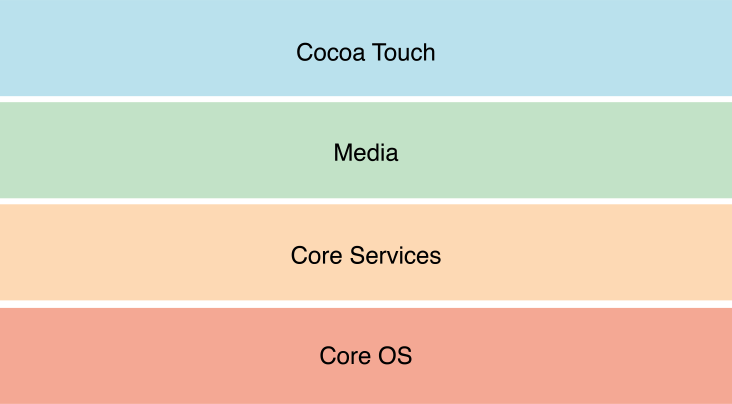
\includegraphics[width=1.0\textwidth]{iOS_SystemLayers.png}
\caption{Platforma iOS, systémové vrstvy \cite{ios_technology_overview}}
\label{fig:iOSSystemLayers}
\end{figure}

Vývojářům je obecně doporučováno využívat co nejvíce technologií z vyšších vrstev této architektury, neboť se jedná o objektové zabstraktnění nízkoúrovňových konceptů.

\subsection{Aplikační technologie}
O celý postprocesing a slinkování hotové aplikace se v iOS starají LLVM (Low Level Virtual Machine) a frontend Clang \cite{bp_dominik}. 

LLVM je kompilátorová infrastruktura pro „Compile Time“, „Link Time“ a „Run Time“, jejíž infrastruktura se dělí na front-end a back-end. Úkolem front-endu je vygenerování bytecodu srozumitelného pro back-end. Back-end následně bytecode zkompiluje do nativního strojového kódu \cite{bp_dominik}. 

Cang je front-end kompilátor pro céčkové programovací jazyky. V našem případě se používá především pro kompilaci jazyka Objective-C o němž si povíme později.

\subsection{Vývojářské technologie}
Aplikace pro systém iOS se programují primárně v jazyce Objective-C \cite{introduction_ios_development}. Objective-C je objektově orientovaný, reflektivní jazyk, v němž lze nalézt společné rysy se známým jazykem SmallTalk \cite{bp_dominik}. Poměrně složitá syntaxe Objective-C představuje značnou překážku pro začínající vývojáře, protože se výrazně liší od ostatních běžně používaných jazyků (například Javy v Androidu).

Díky kompilační struktuře naznačené v předchozí kapitole můžeme však místo Objective-C použít alternativní programovací jazyky, pokud k nim najdeme vhodný front-end. Toho využívá například projekt Monotouch, který vám umožňuje programovat nativní aplikace v C\# a frameworku .NET \cite{xamarin_monotouch}.

\subsection{Vývojářské nástroje}
Apple dává vývojářům k dispozici balík iOS SDK, který obsahuje široké spektrum nástrojů potřebných k tvorbě nativních aplikací pro systém iOS. Tento balík obsahuje například vývojové prostředí XCode, emulátor pro simulovaný běh aplikací na virtuálním zařízení, nástroj pro designování grafických prvků navrhované aplikace, offline verzi dokumentace a mnoho dalšího.

Pro vývoj aplikací pro iOS je nutné vlastnit počítač s operačním systémem Mac OS X. Toto je další poměrně značná překážka pro začínající vývojáře neboť počítače s tímto systémem jsou prozatím na trhu zastoupeny v marginální míře a konkurence v podobě Androidu umožňuje vyvíjet aplikace pro tento systém na libovolné platformě.  Pro publikování aplikací v tržišti App Store je navíc potřeba vlastnit placený vývojářský účet \cite{distribute_ios_app}.

\section{Platforma Android}
\subsection{Systémová architektura}
Architektura operačního systému Android je rovněž vrstevnatá. Jak vidíme na obrázku \ref{fig:AndroidArchitecture}, nejníže se nachází jádro, které se stará o přímou komunikaci s hardwarem zařízení. Android používá jádro Linux verze 2.6, které Google upravil k obrazu svému \cite{android_architecture}. Toto jádro obsahuje ovladače k jednotlivým součástem hardwaru, jako je například fotoaparát, baterie, SD karta a podobně. Zároveň poskytuje vyšším vrstvám rozhraní, pomocí kterého může vývojář hardwarové funkce využít ve svých aplikacích. Android využívá Linux i pro další životně důležité systémové funkce jako je správa pamětí, management procesů, zabezpečení apod.

Nad jádrem leží vrstva knihoven. Tyto knihovny slouží pro práci s různými datovými strukturami a jsou modifikovány zařízení od zařízení. Knihovny jsou napsány v jazyce C či C++. Mezi těmi nejzajímavějšími můžeme zmínit například knihovnu pro práci s databází SQLite či jádro Webkit, jehož prací je správné zobrazování HTML souborů.

Další vrstvou je tzv. Application framework. S tou přijde vývojář do styku nejvíce, neboť zde se nachází většina volání, kterých bude ve svých aplikacích využívat. Application framework se sestává z tzv. bloků, přičemž každý jeden blok slouží k jinému účelu. Za zmínku stojí například Telephony manager, který se stará o správu telefonních hovorů. Můžeme tohoto bloku využít, pokud budeme chtít uživateli umožnit telefonování přímo z aplikace. Neméně důležitý je také Location Manager, jehož úkolem je zjišťování polohy zařízení především pomocí GPS modulu.

Nejvýše v celé hierarchii se nachází vrstva se samotnými aplikacemi. V této vrstvě se vyskytují, krom systémových aplikací jako je Home screen či Kontakty, i uživatelské aplikace.

\begin{figure}\centering
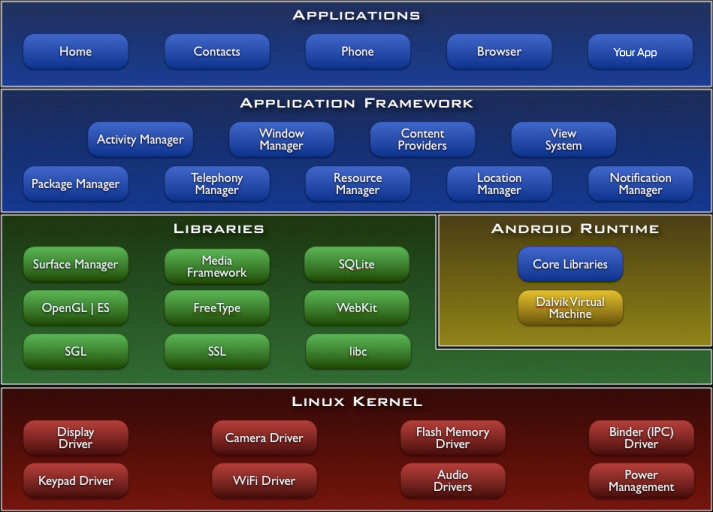
\includegraphics[width=1.0\textwidth]{Android-architecture.jpg}
\caption{Architektura systému Android \cite{android_architecture}}
\label{fig:AndroidArchitecture}
\end{figure}

\subsection{Aplikační technologie}
Nativní aplikace běží ve virtuálním prostředí zvaném Dalvik Virtual Machine. Jedná se o open-source variantu známější Java Virtual Machine, nicméně DVM je speciálně uzpůsobena pro běh na méně výkonných zařízeních, jako jsou právě mobilní telefony \cite{android_architecture}. Každá aplikace běží v instanci tohoto DVM a celá tato instance běží uvnitř Linuxového procesu, který komunikuje přímo s jádrem \cite{introduction_android_development}.

\begin{figure}\centering
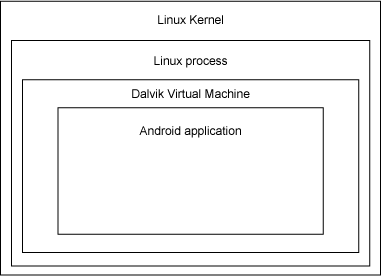
\includegraphics[width=0.6\textwidth]{android_app_tech.png}
\caption{Architektura systému Android 2 \cite{introduction_android_development}}
\label{fig:AndroidArchitecture2}
\end{figure}

\subsection{Vývojářské technologie}
Pro vývoj nativních aplikací se používá programovací jazyk Java. Podle společnosti TIOBE se jedná o druhý nejpoužívanější programovací jazyk na světě \cite{tiobe_software}. Java je objektově orientovaný jazyk se syntaxí blízkou jazykům C a C++.

Velkou výhodou Javy je její platformní nezávislost. Vlastní kód se totiž překládá do tzv. mezikódu, který je poté interpretován v rámci Java Virtual Machine \cite{understanding_jvm_internals}. Program napsaný v Javě je tak spustitelný na Windows, Mac OS X i Linuxu.

\subsection{Vývojářské nástroje}
Google, podobně jako Apple, připravil pro externí vývojáře balík všeho potřebného pro vývoj nativních aplikací, tzv. Android SDK. Ten obsahuje velmi populární vývojové prostředí Eclipse IDE obohacené o plugin ADT (Android Developer Tools). Toto rozšíření se stará o hlubokou integraci nástrojů samotného SDK do vývojového prostředí. Poskytuje tak GUI přístup například k debugovacím nástrojům (DDMS), návrhovým nástrojům pro uživatelské rozhraní, přístup a konfiguraci emulátorů a podobně.

Součástí SDK jsou samozřejmě i zdrojové kódy nejnovější verze systému Android a také obraz systému spustitelný v emulátoru. Nechybí ani podrobná dokumentace pro offline použití.

\section{Platforma Windows Phone}
V této podkapitole se hodlám věnovat pouze nejnovější verzi platformy Windows Phone – Windows Phone 8, protože se její architektura značně odlišuje od předchozí sedmé verze.

\subsection{Systémová architektura}
Když společnost Microsoft uváděla osmou verzi svého operačního systému pro chytré telefony na trh, jednou z hlavních deklarovaných předností mělo být jádro, které sdílí velké části kódu s desktopovou verzí systému Windows – Windows 8 \cite{announcing_wp8}.Tato změna měla přinést mnoho vlastností z „dospělého“ operačního systému na mobilní úroveň. Jedná se například o podporu vícejádrových procesorů, podporu NFC, podporu displejů s různým rozlišením a podobně.

\begin{figure}\centering
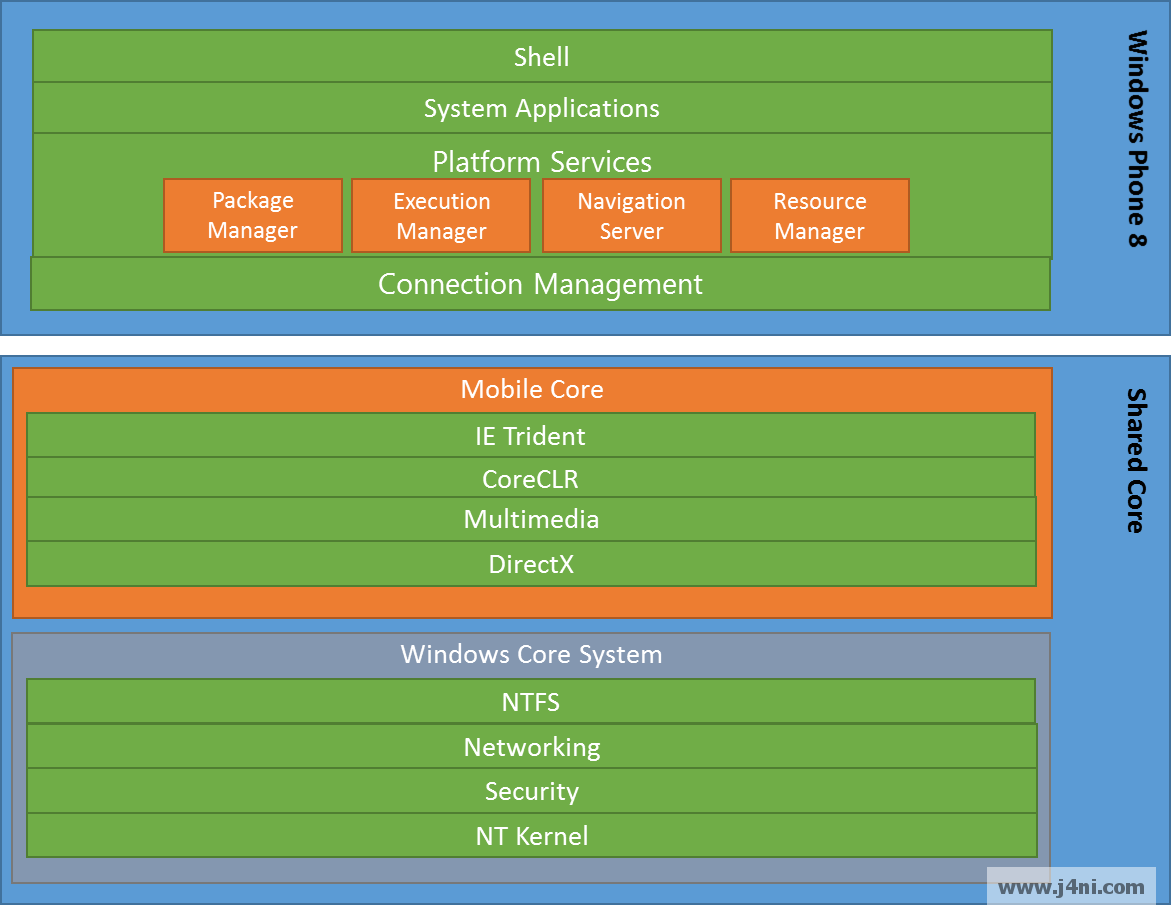
\includegraphics[width=1.0\textwidth]{WP8Architecture.png}
\caption{Architektura systému Windows Phone 8 \cite{wp8_kernel_architecture}}
\label{fig:WP8Architecture}
\end{figure}

Na obrázku \ref{fig:WP8Architecture} vidíme sdílenou část jádra nazvanou „Windows Core System“. Jedná se o klíčovou část jádra systému Windows Phone a nachází se zde nejdůležitější systémové funkce, jako je podpora NTFS filesystému, bezpečnostní funkce, podpora pro síťování apod \cite{wp8_kernel_architecture}. 

Sekce nazvaná „Mobile Core“ obsahuje také značnou část kódu sdílenou s dospělými Windows, nicméně je již mírně modifikovaná pro mobilní použití \cite{wp8_kernel_architecture}. V této části jádra se nachází například srdce internetové prohlížeče Trident, podpora pro přehrávání mutlimédií a podobně.

Nad jádrem se nachází vrstva se systémovými aplikacemi, jako je People Hub, přehrávač hudby a videa, dále vrstva Windows Phone Shell, Connection Management a tzv. Platform Services. Volání z této vrstvy využívají všechny uživatelské aplikace. Nachází se zde například Package manager, který se stará o celý životní cyklus aplikace od nainstalování po její odstranění. Dále zde najdeme Resource manager, který sleduje jaká aplikace využívá které systémové prostředky a do jaké míry \cite{wp8_kernel_architecture}. V případě problémů může „neposlušnou“ aplikaci ukončit.

\subsection{Aplikační technologie}
U předchozí verze Windows Phone si uživatelé často stěžovali na dlouhou prodlevu při spouštění aplikací. To bylo zapříčiněno především způsobem kompilace, který byl použit. Aplikace se zkompilovávala za běhu znovu a znovu podle toho, jaké funkce uživatel používal \cite{wp8_compile_cloud}. Tento postup byl příčinou často pomalých a těžkopádných aplikací.

U nové verze systému se Microsoft pokusil tento problém vyřešit. Zvolil metodu, kterou nazývá „Compile in the Cloud“. Průběh celého procesu je vidět na obrázku \ref{fig:WP8Compilation}. 

\begin{enumerate}
	\item Vývojář zkompiluje aplikaci pomocí C\# překladače a ta se přeloží do mezijazyka.
	\item Tento obraz nahraje do Windows Phone Store, kde je v průběhu nahrávání zkompilován MDIL překladačem do dalšího mezijazyka – Machine Dependent Intermediate Language.
	\item Uživatel si stáhne obraz aplikace právě v kódu MDIL.
	\item Linker při každém spuštění aplikace ověří závislosti a dovede převod do finálního strojového kódu.
\end{enumerate}

V čem je výhoda tohoto řešení? Mezijazyk MDIL je velmi podobný finálnímu strojovému kódu. Zásadní odlišností je nahrazení některých potenciálně rizikových částí symboly, které jsou doplněny až při slinkování finální aplikace \cite{wp8_compile_cloud}. Například při aktualizaci telefonu mohou být porušeny některé závislosti, na kterých aplikace závisí. Při jejím spuštění to však Linker snadno odhalí a aktualizuje příslušné části nativního kódu.

Aplikace samotná pak běží jako samostatný proces, který se může necházet v několika stavech: 1. běžící, 2. spící, 3. tombstone (zombie).

\begin{figure}\centering
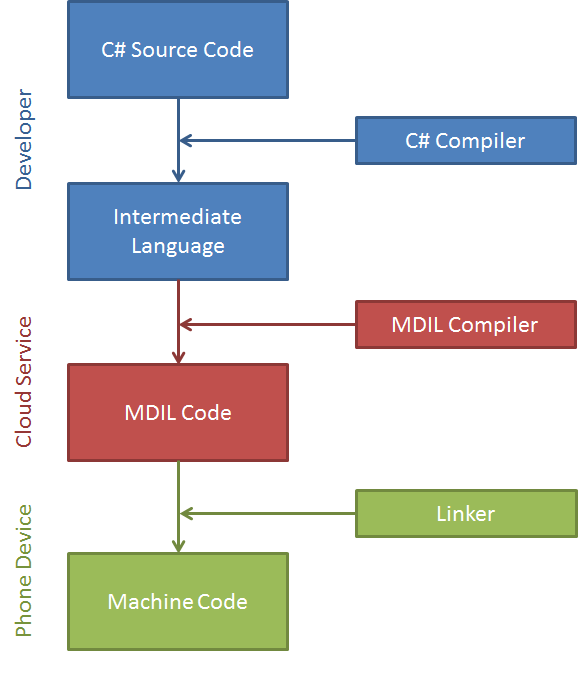
\includegraphics[width=1.0\textwidth]{wp8_cloud_compilation.png}
\caption{Průběh sestavení aplikace pro systém Windows Phone 8 \cite{wp8_compile_cloud}}
\label{fig:WP8Compilation}
\end{figure}

\subsection{Vývojářské technologie}
Pro vývoj aplikací pro systém Windows Phone 8 (ale i pro desktopové Windows) se primárně používá jazyk C\#. Tento jazyk byl vyvinutý spolu s frameworkem .NET firmou Microsoft. C\# je objektově orientovaný jazyk, u jehož syntaxe se Microsoft inspiroval u programovacích jazyků z rodiny C. Některé aspekty však přejal také z oblíbené Javy.

Framework .NET je komplexní balík knihoven a rozhraní určených pro vývoj, kompilaci a spouštění aplikací pro platformu Windows.

\subsection{Vývojářské nástroje}
Také pro platformu Windows Phone 8 existuje balík nástrojů určený pro vývoj nativních aplikací – Windows Phone 8 SDK. Jeho součástí je odlehčená verze Microsoft Visual Studia – Visual Studio Express 2012. Visual Studio je velmi oblíbené vývojové prostředí s širokým spektrem funkcí, jež sou vývojářům k dispozici. SDK obsahuje množství nástrojů pro návrh, testování, debugování a emulátory pro běh uživatelských aplikací.

\section{Platforma Firefox OS} \label{Sec:FxOS}
\subsection{Systémová architektura}
Jak můžeme vidět na obrázku \ref{fig:FxOSArchitecture}, architekturu platformy Firefox OS můžeme rozdělit do tří hlavních vrstev \cite{fxOs_architecture}.

\begin{enumerate}
	\item Gonk je nejnižší vrstva systému. Jeho součástí je jádro operačního systému Linux, které se stará o komunikaci s hardwarem zařízení. Dále v této vrstvě najdeme open-source knihovny pro práci s USB (libusb), pro komunikaci pomocí Bluetooth a podobně. Některé knihovny jsou dokonce přejaté z operačního systému Android (GPS, fotoaparát atd.) \cite{fxOs_architecture}. Můžeme zjednodušeně říci, že Gonk je distribucí operačního systému Linux.
	\item Gecko není jen jádrem prohlížeče Firefox, ale i srdcem systému Firefox OS. Ve Firefox OS nalezneme Gecko portované speciálně pro „distribuci“ Gonk. Gecko přináší podporu pro základní webové technologie (HTML, CSS, JavaScript), které vývojáři používají pro vývoj nativních aplikací pro systém Firefox OS. Součástí této vrstvy je i řada otevřených standardů WebAPI, na jejichž vývoji pracuje společnost Mozilla. Jejich cílem je standardizovat (W3C) webová volání, jež budou poskytovat jednotný přístup vývojářům webových mobilních aplikací (a dokonce i obyčejných webových stránek) k hardwarovému vybavení telefonu. Součástí tohoto WebAPI je již celá řada volání, které vývojáři používají při vývoji svých aplikací pro Firefox OS. Patří mezi ně například volání na ovládání Geolokace, Kontaktů, Fotoaparátu a podobně. Více o WebAPI si řekneme v kapitole XY. % TODO ověřit
	\item Gaia je nejvyšší vrstvou systému Firefox OS. Gaia má na starost vše okolo zobrazování uživatelského rozhraní. Domovská obrazovka, lock screen a všechny systémové aplikace jsou vytvořeny a spravovány právě pomocí Gaii. Samotná Gaia je v duchu filozofie systému Firefox OS napsaná čistě v HTML, CSS a JavaScriptu \cite{fxOs_architecture}. Uživatelské aplikace se instalují vedle této vrstvy.
\end{enumerate}

\begin{figure}\centering
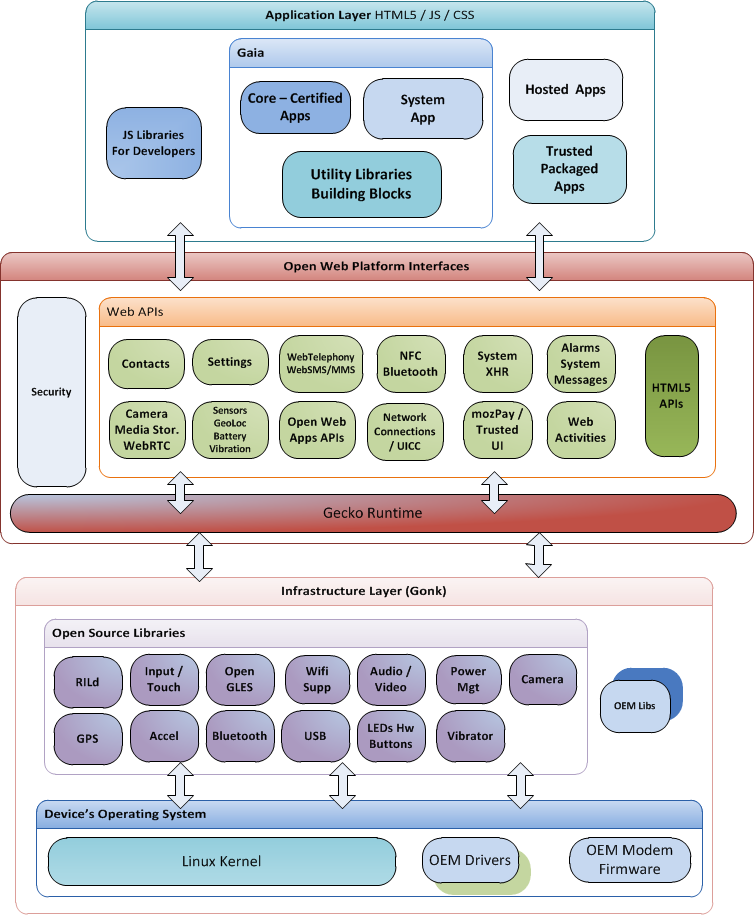
\includegraphics[width=1.0\textwidth]{FirefoxOS_architecture.png}
\caption{Architektura systému Firefox OS \cite{fxOs_architecture}}
\label{fig:FxOSArchitecture}
\end{figure}

\subsection{Aplikační technologie}
Protože nativní aplikace pro systém Firefox OS není nic jiného než „trochu vylepšená“ webová stránka (přesněji tzv. Open Web App \cite{faqs_mozilla}), nemůžeme od Firefox OS očekávat jakýkoliv proces kompilace.

Taková webová aplikace může samozřejmě fungovat jako běžná webová stránka uvnitř internetového prohlížeče. Uživatelé ovšem obvykle očekávají od mobilní aplikace více než od webové stránky. Aplikace ve Firefox OS běží mimo internetový prohlížeč. Ke svému běhu využívají tzv. Web runtime. Web runtime je software obsažený v internetovém prohlížeči, který však může běžet samostatně a zajišťuje celý životní cyklus aplikace od jejího spuštění, po obsluhu jejích požadavků až po její ukončení uživatelem \cite{apps_architecture}.

\subsection{Vývojářské technologie}
Jelikož jsme již naznačili, že pro vývoj nativních aplikací pro Firefox OS se používají pouze webové technologie dnes souhrnně (nesprávně?) označované jako rodina HTML5, do kterých řadíme:

\begin{enumerate}
	\item HTML5 jako značkovací jazyk ve své páté (dosud neoficiální) verzi obohacen o mnohé moderní funkce jako je geolokace, lokální databáze či nativní podpora pro přehrávání videa a audia.
	\item CSS3 pro definici vzhledu a částečně i chování uživatelského rozhraní aplikace.
	\item JavaScript je interpretovaný programovací jazyk, který se používá pro zajištění aplikační logiky. Jeho syntaxe se inspirovala u programovacích jazyků C/C++ a Java.
\end{enumerate}

\subsection{Vývojářské nástroje}
Mozilla nenabízí vývojářům aplikací pro Firefox OS (který stále ještě není v oficiálním prodeji) žádný balík se vším potřebným jako je tomu u jiných platforem. Důvodem pro tento fakt je pravděpodobně všudypřítomnost vývojářských nástrojů pro webové stránky/aplikace.

Přesto však firma Mozilla na konci roku 2012 vydala emulátor systému Firefox OS, na kterém mohou vývojáři testovat své aplikace aniž by museli vlastnit reálné zařízení. Firefox OS Simulator existuje pro Windows, Mac i Linux a lze jej dokonce získat i jako plugin do desktopové verze internetového prohlížeče Firefox \cite{announcing_fxOS_simulator}.

% Kapitola Multiplatformní vývoj
\chapter{Multiplatformní vývoj}
	\section{Co je to multiplatformní vývoj?}
Multiplatformní vývoj je nadále žhavým tématem v diskuzích uvnitř komunit vývojářů desktopových i mobilních aplikací. Jedná se o přístup, který umožňuje vývojářům napsat program jednou, ale být jej schopen spouštět na více platformách. Pro splnění definice však již není podstatné, na kolika platformách může program běžet, pakliže je jich více než jedna. Tedy i aplikace, která dokáže běžet pouze na dvou platformách, je z hlediska této definice multiplatformní.

Na tomto místě by šlo namítnout, že i aplikace, která je napsána pro každou platformu zvlášť, je multiplatformní, neboť jí lze spouštět na více systémech. Je to do jisté míry pravda, nicméně pokud se na to podíváme z jiného úhlu, můžeme takový přístup označit za vývoj aplikací, které se podobají, ale nejedná se o programy totožné.

Multiplatformní přístup je tedy způsob, jak využít jeden zdrojový kód, který jsme schopni provozovat (s minimálními úpravami) na různých platformách a operačních systémech. Pro tento přístup se v angličtině vžilo heslo „write once, run everywhere“. 

Jedním z často používaných dělících kritérií, pomocí kterých můžeme multiplatformní software rozlišovat, je kritérium způsobu jejich kompilace a následného běhu na samotné platformě.

\begin{enumerate}
	\item Zdrojový kód je nutno zkompilovat pro každou platformu zvlášť. Poté je tedy nutno udržovat repozitář s různými instalačními balíčky pro jednotlivé platformy.
	\item Zkompilování zdrojového kódu pouze jedinkrát a jeho následný běh na uživatelově platformě pomocí nějakého interpreteru či run-time prostředí, které je součástí systému.
\end{enumerate}

Příkladem multiplatformních aplikacích je  vývojářské prostředí Eclipse, internetový prohlížeč Opera, Google Earth apod.

Jak již bylo řečeno, způsobů jak multiplatformně vyvíjet je mnoho. Pro tvorbu multiplatformní desktopové aplikace je možno využít standardního programovacího jazyka (pro který existuje kompilátor na více platformách) spolu s frameworkem, který umožňuje multiplatformní vývoj (nejen) GUI. Mezi takové UI toolkity můžeme zařadit například Qt, wxWidgets nebo GTK+. 

Kapitola sama pro sebe je Java. Java je platformou umožňující vývoj aplikací zcela nezávislých na operačním systému. Tato technologie je skutečným zosobněním přístupu „write once, run everywhere“. Nutno však v zápětí dodat, že „everywhere“ je omezeno přítomností Java Virtual Machine. Programy napsané v Javě totiž nejsou závislé na konkrétním operačním systému, ale právě na speciálním prostředí (JVM), které zdrojový kód (Java bytekód) interpretuje.

Ačkoliv je Java velmi oblíbenou vývojářskou platformou, nestala se nikdy všudypřítomnou technologií, která překoná rozdíly mezi platformami, jak se mnozí domnívali. O důvodech můžeme spekulovat. Jedním z nich je zcela nepochybně nenativní chování javovských aplikací. Programy v Javě totiž na dané platformě málokdy působí jako nativní aplikace, což představuje značnou překážku k jejich širokému přijetí. I přes snahy o řešení (například pomocí knihovny Java Swing) se tento problém stále nepodařilo zcela překonat.

Nezřídkakdy se můžete setkat s názorem, že „HTML5 je nová Java“ \cite{why_html5_java}. Toto tvrzení vychází zejména z faktu, že HTML5, stejně jako Java, splňuje paradigma „write once, run everywhere“. Na rozdíl od Javy je však vývoj v HTML5 podstatně jednodušší a výkon aplikací se neustále zlepšuje (zejména díky výkonnějším JavaScriptovým enginům v internetových prohlížečích). Další předností HTML5 aplikací je jejich snadná dostupnost pro koncového uživatele. Nemusí instalovat víc než webový prohlížeč a znát tu správnou URL. 

Zásadním argumentem, proč je HTML5 novou Javou, je však podle mě něco jiného. Je to zejména dramatický nástup mobilních zařízení. „Write once, run everywhere“ pro javovské aplikace v mobilním světě neplatí. Z předních hráčů na trhu se Java Virtual Machine vyskytuje pouze na Androidu, na ostatních platformách si tudíž javovské aplikace nespustíte. Naopak HTML5 je díky všudypřítomnosti webového prohlížeče skutečně multiplatformní technologií i z pohledu mobilního světa. 

Samozřejmě by někdo mohl namítnout, že porovnávání Javy a HTML5 poněkud kulhá, neboť funkcionalita, kterou dává vývojářům k dispozici Java, je oproti HTML5 obrovská. Avšak HTML5 obsahuje (a nadále přidává) zejména ty funkce, které najdou uplatnění i v chytrých mobilních telefonech. A z těch již zase tak mnoho nechybí. HTML5 přebírá pozici Javy právě proto, že je úspěšné i na poli mobilních telefonů.

\section{Argumenty pro multiplatformní přístup}
V této části bych se rád podrobněji zaměřil na důvody, které vedou vývojáře k zahrnutí multiplatformního řešení do svých úvah. Pokusím se zde nastínit argumenty, které se v této souvislosti nejčastěji skloňují.

\subsection{Možnost cílit na široké spektrum platforem najednou}
Tento důvod byl podle výzkumu společnosti VisionMobile uváděn vývojáři nejčastěji. 60 \% z nich konstatovalo, že právě širší záběr, který jim multiplatformní přístup přináší, je přesvědčil k využití některého z multiplaformních nástrojů. \cite{visionmobile_survey}

Velké společnosti stojící za platformami jako je Android či iOS se velmi snaží, aby vývojáři vyvíjeli exkluzivně pro jejich platformu. Přítomnost těch nejžádanějších aplikací výhradně pro jednu platformu jí totiž přináší značnou konkureční výhodu na trhu. V zájmu těchto hráčů proto není, aby bylo možné aplikace snadno vyvíjet na více platforem najednou. Naopak méně rozšířené systémy jako je Windows Phone, Samsung Bada, RIM a další mají eminentní zájem na tom, aby bylo pro jejich systém dostupné co největší množství aplikací bez zbytečného čekání. Takzvaný „time-to-market“ je totiž u těchto platforem často mnohem větší než u velkých hráčů, protože nativní vývojáři se logicky snaží prvně zasáhnout co největší část trhu, která je okupována právě iOS a Androidem. 

Možnost rychle zasáhnout tzv. „long tail“ je tedy pro vývojáře velice lákavá. Mohou bez zbytečných prodlev rychle oslovit prakticky celý trh a nemusí tak dávkovat marketingovou podporu podle toho, na které platformě jejich aplikace právě běží. O jejich aplikaci mohou mluvit všichni.

\subsection{Nižší náročnost na zdroje}
Náročnost na zdroje je klíčový faktor zejména pro společnosti, které aplikace vyvíjejí. Pokud chtějí být s aplikací opravdu úspěšní, musí s ní oslovit co nejširší spektrum uživatelů. To v dnešní době znamená mít verzi pro iOS, Android a Windows Phone. Dělat nativní aplikaci pro každý z těchto systémů znamená platit tři týmy vývojářů, protože pro každou platformu se programuje jiným programovacím jazykem, systém má jiná API volání a podobně. Zároveň je velmi neobvyklé, aby jeden vývojář ovládal na solidní úrovni technologie pro všechny tři platformy.

Ale problém není jen v kódování. Vyvíjet pro tři různé platformy znamená udržovat tři různé sady zdrojových kódů, trackování bugů pro každou z nich zvlášť a podobně. Zároveň účinná synchronizace mezi týmy klade další požadavky na lidské zdroje. Zajistit, aby všechny tři verze měly stejné vlastnosti, dodržovaly stejná designová paradigmata a zároveň se neodchylovaly od časového harmonogramu, je poměrně obtížný úkol.
\\ \\
\textit{\uv{Zjistili jsme, že použitím multiplatformního nástroje jsme schopni v průměru zredukovat náš ‚time to market‘ o 70\%,}} tvrdí Paulius Uza, výkonný ředitel společnosti InRuntime \cite{visionmobile_survey}.
\footnote{“We have found that by using cross-platform tools our time to market is reduced by 70\% on average,” remarks Paulius Uza, CEO of development house InRuntime \cite{visionmobile_survey}.}	

\subsection{Nižší finanční náročnost}
S předchozím bodem přímo souvisí i nižší finanční náročnost. Je zřejmé, že když budete zaměstnávat méně vývojářů, kteří pro vás aplikaci vyvíjejí, i vaše náklady budou nižší. Není to však jen o samotném vývoji. Po vypuštění hotové aplikace na trh je nutno zajistit podporu pro její uživatele. Z hlediska rozpočtu je značný rozdíl, zda-li musíte obhospodařovat jednu sadu se zdrojovými kódy nebo tři.

Podle společnosti VisionMobile stojí vývoj pro každou další platformu v průměru 50 \% původních nákladů \cite{visionmobile_survey}. Nejedná se tedy rozhodně o malé částky a každou rozpočtově odpovědnou firmu tento fakt nutí k zamyšlení, jak vyvíjet pro více platforem levněji.

\subsection{Menší vstupní bariéry}
K tomuto argumentu si nejprve uveďme dvě poznámky. Zaprvé, jazyky, ve kterých se vyvíjí nativní aplikace jsou poměrně obtížné na naučení. Názorným příkladem je v tomto ohledu Objective-C, který se vyznačuje nejen poměrně neobvyklou syntaxí, ale zároveň obsahuje množství značně neobvyklých návrhových vzorů a doporučení, která jsou poměrně obtížná na pochopení. I to je důvodem, proč je na trhu v současnosti převis nabídky nad poptávkou po vývojářích mobilních aplikací.

Neméně důležitým faktorem je poměrně široká masa webových vývojářů, která se na trhu vyskytuje. Webové technologie jsou v současnosti velmi oblíbené a to především díky strmému nárůstu popularity celého Internetu v minulé dekádě. Vývoj pomocí webových technologií je poměrně jednoduchý, neboť se při něm vývojář pohybuje na vysoké úrovni abstrakce. Díky tomu je možno vyvíjet webové aplikace rychle a levně.

Tohoto faktu šikovně využívají tvůrci multiplatformních řešení. Snaží se zasáhnout právě široké obecenstvo v řadách webových vývojářů tím, že maximálně snižují vstupní bariéry, které by jim mohly bránit ve vývoji mobilních aplikací. Drtivá většina multiplatformních nástrojů proto využívá pro vývoj mobilních aplikací právě webové technologie HTML, CSS a JavaScript. Pro přístup k nativním funkcím telefonu nabízí tyto nástroje jednoduchá API. Že se jim tento přístup vyplací, dokládá i výzkum společnosti VisionMobile, který zjistil, že více jak 60 \% vývojářů, kteří využívají některý z multiplatformních nástrojů, má více jak 5 let zkušeností s webovým vývojem. Stejně tak při pátrání po důvodech, které vedly vývojáře k využití některého z multiplatformních nástrojů, byla jako druhá nejčastější odpověď uváděna právě možnost využít již naučené technologie \cite{visionmobile_survey}.

\section{Slabiny multiplatformního přístupu}
Pokud zmiňujeme přednosti multiplatformního přístupu, neměli bychom zapomínat ani na slabiny, které stále brání jeho širšímu rozšíření.

\subsection{Slabší výkon}
Slabší výkon je nejčastěji uváděným důvodem pro zavržení multiplatformního nástroje \cite{visionmobile_survey}. Vzhledem k tomu, že drtivá většina multiplatformních nástrojů závisí na nějaké mezivrstvě (ať už je to jakýsi most u hybridních aplikací, nebo runtime), není slabší výkon takto vytvořených aplikací příliš překvapivý.

Svojí strastiplnou zkušenost s multiplatformním přístupem si zažil i gigant na poli sociálních sítí – společnost Facebook. Ve svých mobilních aplikacích pro platformy iOS a Android kombinoval technologii HTML5 s nativními prvky. Výsledkem byla pomalá aplikace a velmi špatná uživatelská hodnocení na oficiálních tržištích. Po přechodu na čistě nativní technologie se používanost těchto aplikací pro konzumaci obsahu z Facebooku zdvojnásobila. \cite{zuckerberg_biggest_mistake,facebook_android_obal} \\ \\

\textit{\uv{Když se podívám pár let nazpět, tak za největší chybu, kterou jsme jako společnost udělali, bych označil přílišné sázení na HTML5 oproti nativním technologiím. HTML5 prostě ještě není připravené.}} Mark Zuckerberg \cite{html5_isnt_fb_mistake}
\footnote{“When I'm introspective about the last few years, I think the biggest mistake that we made as a company is betting too much on HTML5 as opposed to native. Because it just wasn't there.” Mark Zuckerberg \cite{html5_isnt_fb_mistake}} \\

\subsection{Omezený přístup k nativním funkcím zařízení}
Pravdou je, že ze své podstaty budou multiplatformní nástroje vždy o několik kroků pozadu oproti nástrojům pro nativní vývoj. Souvisí to právě s tím, že se multiplatformní nástroje snaží podporovat co nejvíce různých platforem. Z toho důvodu se musí omezovat na průnik množin funkcí, které tyto platformy nabízejí. Velice dobře tento problém popsal Steve Jobs ve svém otevřeném dopise společnosti Adobe „Thoughts on Flash“.
\\ \\
\textit{\uv{Z naší strastiplné zkušenosti víme, že položením vrstvy třetí strany mezi vývojáře a platformu, nevyhnutelně získáme aplikace podprůměrné kvality a vytvoříme tím překážky pro další rozvoj platformy. Pokud se vývojáři naučí být závislí na knihovnách a nástrojích třetí strany, mohou využívat nových vylepšení platformy až ve chvíli, kdy se třetí strana rozhodne je implementovat. Nemůžeme být vydáni na milost třetí straně, až se rozhodne umožnit našim vývojářům používat vylepšení, které v platformě uděláme. \\ \\
Problém se jenom zhorší, pokud třetí strana v rámci svého nástroje podporuje více platforem. Třetí strana pak nemusí implementovat nová vylepšení z jedné platformy až do chvíle, dokud jej neimplementují všechny platformy jež podporuje. Vývojáři aplikací pak mají přístup pouze k nejnižšímu společnému jmenovateli všech funkcí.}} Steve Jobs \cite{thoughts_on_flash}
\footnote{“We know from painful experience that letting a third party layer of software come between the platform and the developer ultimately results in sub-standard apps and hinders the enhancement and progress of the platform. If developers grow dependent on third party development libraries and tools, they can only take advantage of platform enhancements if and when the third party chooses to adopt the new features. We cannot be at the mercy of a third party deciding if and when they will make our enhancements available to our developers.

This becomes even worse if the third party is supplying a cross platform development tool. The third party may not adopt enhancements from one platform unless they are available on all of their supported platforms. Hence developers only have access to the lowest common denominator set of features.” Steve Jobs \cite{thoughts_on_flash}}\\

Nejedná se však pouze o přístup k nativním funkcím, jako je lokální úložiště nebo hardwarové funkce. Jde i o přístup k nativním UI elementům, který u multiplatformních nástrojů často chybí nebo je značně omezený. Vývojáři jsou tak nuceni napodobovat vzhled a chování nativních aplikací pomocí CSS a JavaScriptu, což bývá často složité a má to negativní dopad i na výkon samotných aplikací. Právě omezení v používání nativních UI elementů respondenti uváděli jako druhý nejčastější důvod k zavržení multiplatformního nástroje \cite{visionmobile_survey}.

\subsection{Fragmentace}
Fragmentování neboli tříštění celku je v kontextu mutliplatformního vývoje především problémem webových prohlížečů. Podpora HTML5 standardů se totiž mezi jejich verzemi značně liší. Tento fakt přináší vývojářům časté komplikace, protože mnoho multiplatformních nástrojů používá pro běh aplikací právě prostředí internetového prohlížeče. Na obrázku \ref{fig:HTML5mobilniprohlizece} vidíme, jak moc je podpora standardů mezi prohlížeči roztříštěná. Je z něj patrné, že webový prohlížeč dodávaný se systémem Windows Phone je na tom s podporou HTML5 více než 2x hůře než prohlížeč v systému iOS 5. Problémy s optimalizací webových stránek se tedy přenesly i do světa mobilních aplikací, což vývojáře jistě nepotěší.

\begin{figure}\centering
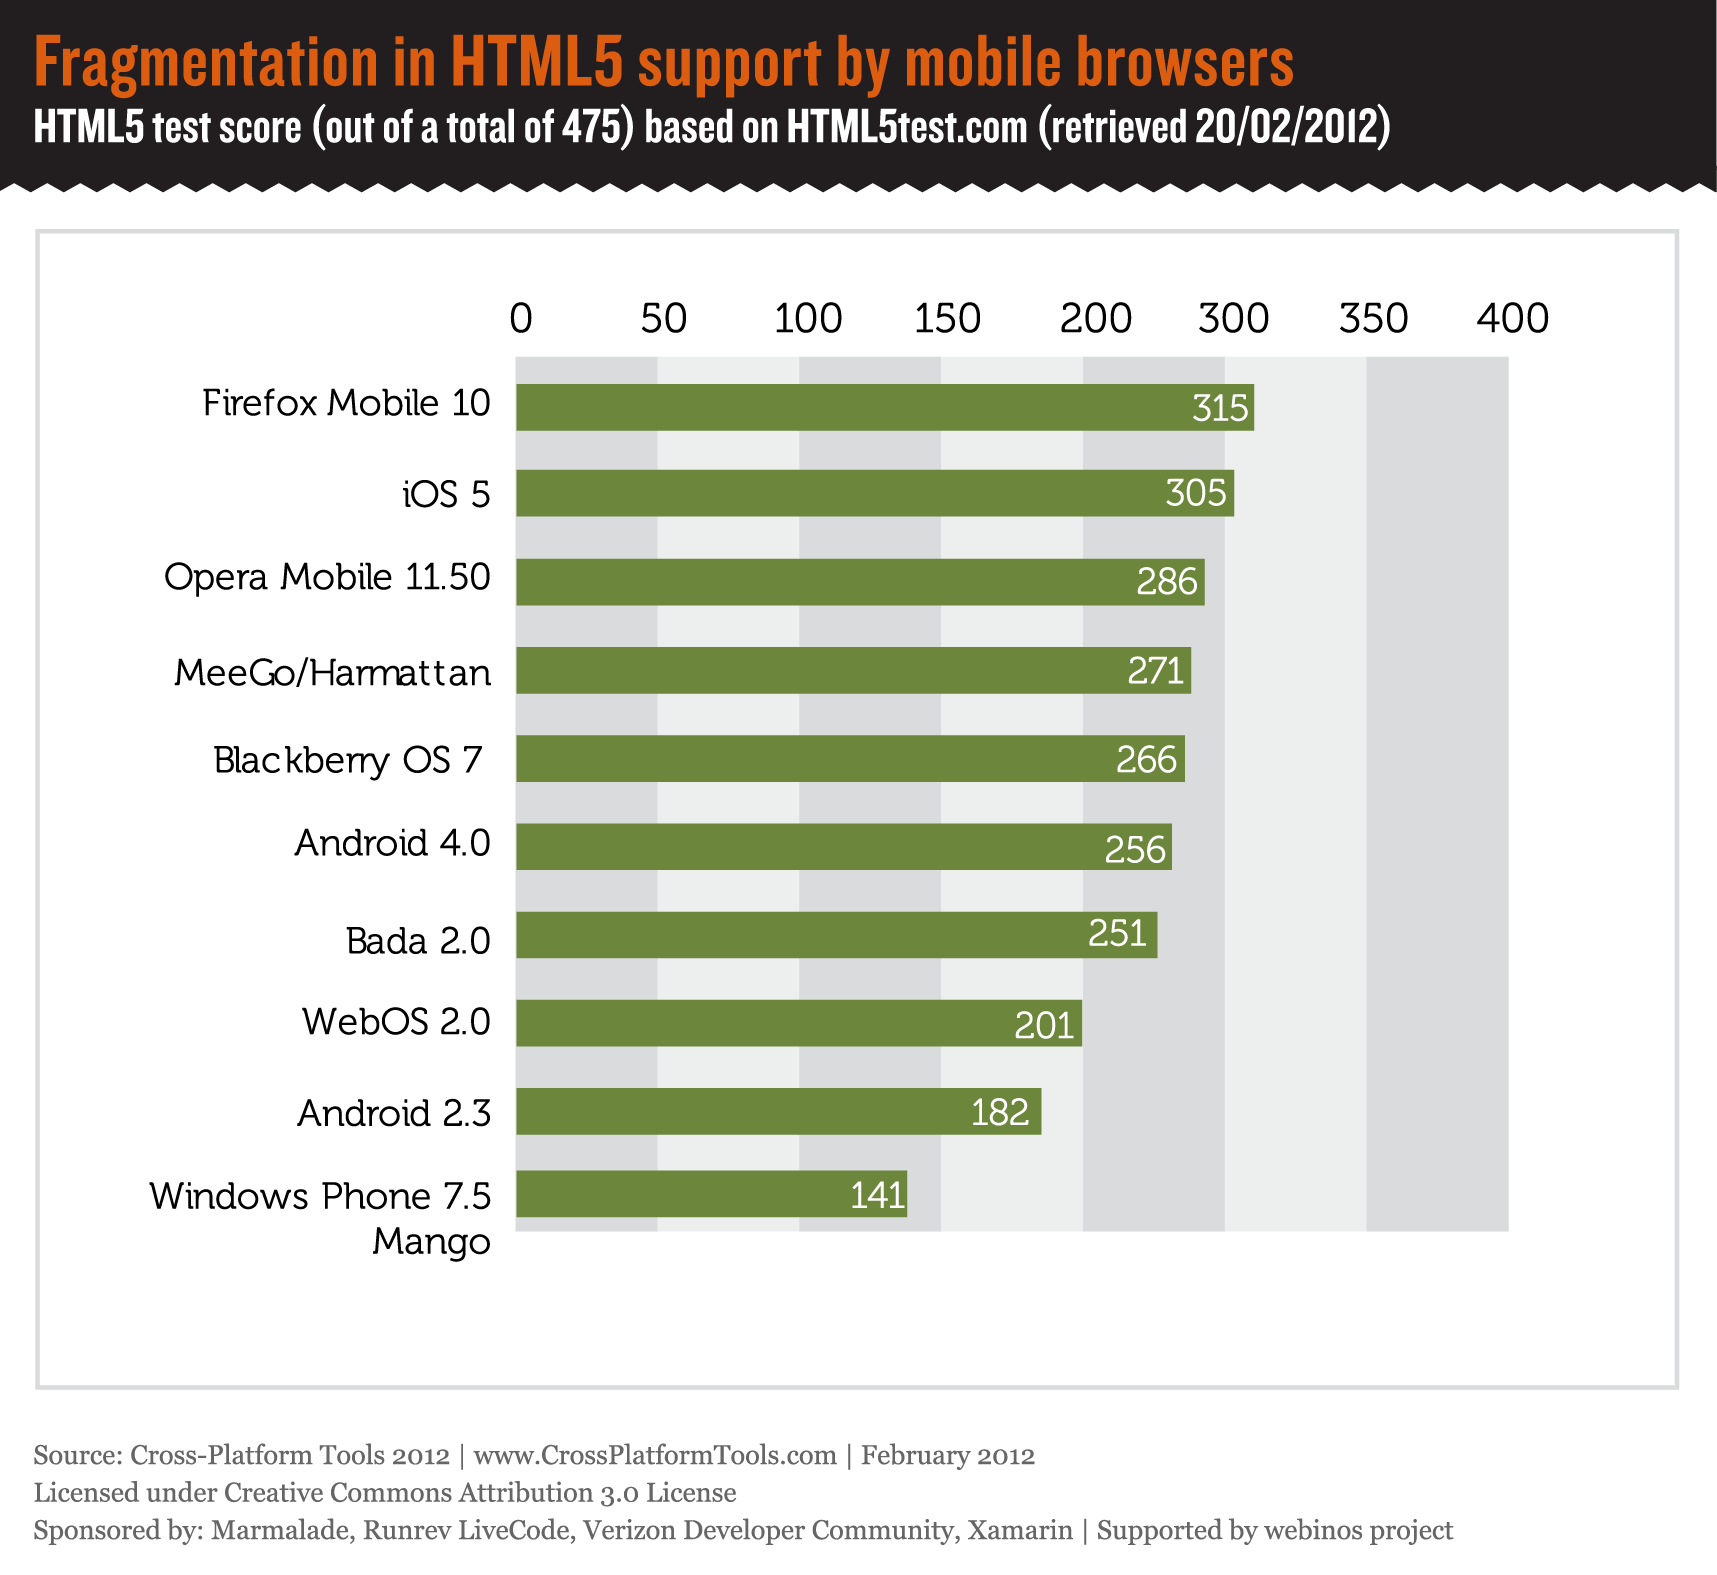
\includegraphics[width=1.0\textwidth]{html5browser.png}
\caption{Podpora HTML5 standardů v mobilních prohlížečích \cite{visionmobile_survey}}
\label{fig:HTML5mobilniprohlizece}
\end{figure}

\subsection{Náročnost vývoje}
I když jsme v benefitech multiplatformního přístupu zmínili, že díky použití webových technologií je samotný vývoj jednodušší, průzkum společnosti VisionMobile prokázal, že právě strmě stoupající náročnost vývoje je častým důvodem k zavržení multiplatformního nástroje \cite{visionmobile_survey}. Zdá se tedy, že s multiplatformními nástroji snadno vyvinete jednodušší aplikaci, ale komplexnější úkoly již představují větší výzvu.

\section{Přístupy k multiplatformnímu vývoji mobilních aplikací}
Dosud jsme hovořili o mutliplatformním vývoji, jako by se jednalo o monolitický celek. V rámci něj však existuje celá řada přístupů, které se od sebe liší technicky i filozoficky. V této části se tedy zaměříme právě na stručný popis těch nejpoužívanějších přístupů, které multiplatformní vývoj nabízí.

\subsection{JavaScriptové frameworky}
Do této rodiny řadíme například známý framework jQuery Mobile či Sencha Touch. Jedná se o frameworky, které umožňují webovým vývojářům snadno vyvíjet dotyková rozhraní svých webových aplikací. Například jQuery Mobile poskytuje možnosti jak definovat vzhled stránky a jednotlivé elementy způsobem, který umožní jejich bezproblémové zobrazení na jakémkoliv dotykovém zařízení. Nesnaží se však simulovat nativní vzhled ovládacích prvků na jednotlivých platformách, narozdíl třeba od nástroje Kendo UI.

\paragraph{Zástupci}
\begin{enumerate}
	\item jQuery Mobile
	\item Sencha Touch
	\item Kendo UI
	\item DHTMX Touch
	\item iUI
	\item Cocos2D (hry)
\end{enumerate}

\subsection{Aplikační továrny}
Aplikační továrny jsou velice moderní přístupem, jak tvořit mobilní aplikace. Slovo „tvořit“ je skutečně na místě, neboť při využití těchto nástrojů není třeba žádných znalostí programovacích jazyků (tedy ani HTML, CSS a JavaScriptu). Aplikace jsou tvořeny uživatelem pomocí skládání vizuálních elementů v nějakém (většinou webovém) WYSIWYG editoru. V případě potřeby může uživatel doplnit chybějící logiku pomocí JavaScriptu.

Jedním z nejznámějších zástupců této skupiny je Tiggzi. Tiggzi je poměrně komplexní nástroj, který v sobě kombinuje JavaScriptový framework jQuery Mobile, webové technologie HTML, CSS a JavaScript a hybridní framework PhoneGap, který umožňuje exportovat aplikace vytvořené v Tiggzi do binárních souborů, které je následně možno publikovat na oficiálních tržištích v rámci jednotlivých platforem.

Tiggzi nabízí uživatelům webový nástroj App builder, kde je možno si velmi jednoduše („drag \& drop“) poskládat uživatelské rozhraní aplikace z předdefinovaných UI komponent. Pokud by vám předdefinovné funkce nestačily, můžete si chybějící funkcionalitu dopsat pomocí JavaScriptu. Díky využití hybridního frameworku PhoneGap může uživatel ve své aplikaci přistupovat k nativním funkcím telefonu. Pro tvůrce aplikací jsou připraveny také nástroje pro snadné připojování k REST API služeb třetích stran. Vaše aplikace tak může snadno získávat data například z Twitteru. Tiggzi dále nabízí nástroje pro testování aplikací, databázové úložiště a další. Je však třeba zmínit, že za použití Tiggzi je třeba zaplatit.

\paragraph{Další zástupci}
\begin{enumerate}
	\item AppMkr
	\item Wix mobile
	\item Spot Specific
	\item Games Salad
\end{enumerate}

\subsection{Hybridní frameworky}
Tento druh multiplatformních nástrojů si popíšeme jen velmi stručně, neboť je mu věnována celá následující kapitola XY. Jedná se o řešení, které umožňuje vývojářům vytvářet aplikace čistě pomocí webových jazyků. Hlavní předností těchto frameworků jsou knihovny napsané v nativních jazycích dané platformy, které vývojářům poskytují tzv. most, pomocí kterého mohou přistupovat k nativním funkcím telefonu jako jsou notifikace, fotoaparát, akcelerometr a podobně. Tyto funkce jsou jim přístupné pomocí JavaScriptového API.
% TODO dodělat reference na kapitoly
Nejznámějším příkladem tohoto přístupu je hybridní framework PhoneGap, kterému se budeme podrobně věnovat v kapitole XY.

\paragraph{Další zástupci}
\begin{enumerate}
	\item Trigger.io
	\item Sencha Touch (v2)
	\item MoSync
\end{enumerate}

\subsection{Runtime}
Tvůrci runtime frameworků se snaží k věci přistupovat trochu jinak. Pokud využíváte takový nástroj, tak vlastně píšete nativní aplikaci, avšak místo nativního jazyka používáte JavaScript. Aplikace se spouští jako nativní, nepotřebuje k tomu prostředníka v podobě webového prohlížeče. Jednou ze zásadních výhod tohoto přístupu je, že při vývoji používáte nativní UI elementy. Není nutné tedy nic napodobovat jako v případě hybridních frameworků a výkon takto napsaných aplikací tak bývá v konečném důsledku rychlejší.

\begin{figure}\centering
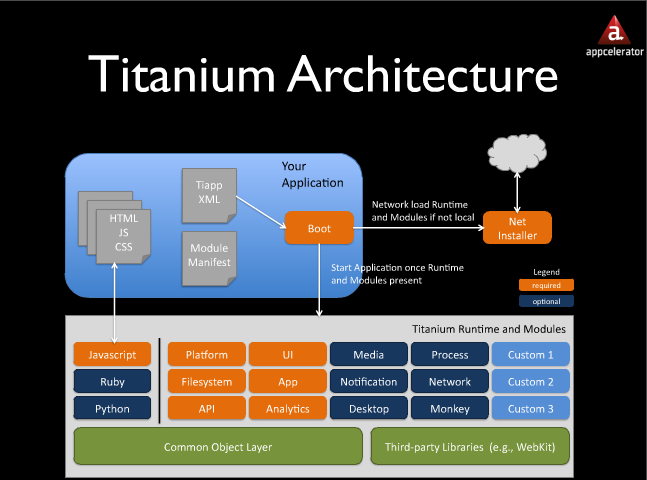
\includegraphics[width=1.0\textwidth]{titanium_architecture.png}
\caption{Architektura runtime frameworku Titanium \cite{architecture_titanium}}
\label{fig:TitaniumArchitecture}
\end{figure}

Pro správné pochopení tohoto principu si můžeme popsat, jak funguje nejznámější zástupce tohoto přístupu – nástroj Appcelerator Titanium. Uživatel v něm píše aplikaci čistě pomocí JavaScriptu, kterýžto zdrojový kód je následně zabalen do nativních binárních souborů určených pro každou z platforem. Při spuštění je použit JavaScriptový interpreter (v iOS JavaScriptCore, v Androidu a Blackberry Mozilla Rhino), který interpretuje váš kód za běhu. Pro volání nativních komponent a hardwarových funkcí telefonu je použito Titanium API, které je napsáno pomocí nativních jazyků a uživatel k němu přistupuje přes volání JavaScriptových funkcí. Appcelerator tvrdí, že 80 \% kódu je možno použít při vývoji mutace aplikace pro jinou platformu \cite{building_apps_titanium}. Hlavním rozdílem oproti hybridním frameworkům je tedy běh aplikací bez nutnosti spouštět webový prohlížeč. O pravé nativní aplikace se však ani v tomto případě nejedná, ač se tím někteří (např. Appcelerator) rádi chlubí. V tomto případě jde spíše o marketingový termín.

Pojďme se seznámit s nástrojem Appcelerator trochu blíže. Krom open-source SDK, které poskytuje více než 5000 API volání pro přístup k nativním prvkům mobilních platforem, je součástí celého řešení i IDE na bázi nástroje Eclipse a MVC framework pro snazší vývoj. Dále je možno využít cloudových služeb pro údržbu a testování aplikací. Pomocí nich lze například posílat push-notifikace, integrovat sociální sítě, posílat e-maily přímo z aplikace apod. Příjemná je i možnost statistického zobrazení dat o používání aplikace uživateli – obdoba Google Analytics. \cite{appcelerator_features} 

Appcelerator se zaměřuje především na webové vývojáře, které se snaží přesvědčit zejména díky lepšímu výkonu oproti aplikacím napsaným pomocí hybridních frameworků jako je PhoneGap \cite{appcelerator_vs_phonegap}. Z výzkumu vyplývá, že uživatelé si vybírají Appcelerator zejména kvůli nízké ceně, přístupu k hardwarovým funkcím telefonu a širokým možnostem úpravy UI jejich aplikace. Naopak velká část z nich by ocenila ještě lepší optimalizaci orientovanou na jednotlivé platformy \cite{visionmobile_survey}.

\paragraph{Další zástupci}
\begin{enumerate}
	\item Adobe Flex/Air
	\item Corona
	\item AppMobi
	\item Unity (Hry)
\end{enumerate}

\subsection{Překladače zdrojových kódů}
Další možností je nechat si přeložit zdrojový kód své aplikace do nativního jazyka dané platformy, případně do nějakého mezikódu či strojového jazyka. Nezřídkakdy jsou překladače zdrojových kódu používány současně s nějakým runtime nástrojem. Tyto nástroje cílí především na zkušené vývojáře, kteří potřebují vyvíjet komplexní aplikace pro více platforem s vysokou úrovní aplikační logiky.

Známým nástrojem z tohoto okruhu je například Marmalade. Marmalade umožňuje vývojářům psát aplikace v jazycích C či C++, který je následně přeložen do nativního jazyka některé z podporovaných platforem. Těch je celá řada, od iOS, Androidu přes Samsung Bada a Blackberry až po dekstopové Windows \cite{marmalade}. Chybí však podpora pro Windows Phone. Pro přístup k nativním funkcím telefonu poskytuje Marmalade SDK API. SDK obsahuje ale i další užitečné nástroje jako je například debugger, UI builder a další.

Podle výzkumu si vývojáři vybírají Marmalade především proto, že je velmi vhodný na vývoj her. Oceňují na něm také vysoký výkon, který jde pravděpodobně na vrub zejména nízké úrovni abstrakce. Na druhou stranu je u uživatelů poptávka po více možnostech licencování. Používání Marmalade je totiž placeno. \cite{visionmobile_survey}

\paragraph{Další zástupci}
\begin{enumerate}
	\item MoSync
	\item Eqela
	\item XMLVM
	\item Bedrock
\end{enumerate}

% Kapitola Hybridní frameworky
\chapter{Hybridní frameworky} \label{Chap:HybridniFrameworky}
	\section{Obecně}
Jak jsem již naznačil v předchozí kapitole, hybridní frameworky jsou nástroje, které umožňují vývojářům mobilních aplikací schovat svojí „webovou aplikaci“ do nativního obalu a na venkovní svět tak působit jako klasická nativní aplikace (více o tom, jak wrappery fungují si řekneme v Technickém popisu v podkapitole \ref{Sec:TechnickyPopis}).

\paragraph{Hlavní přednosti tohoto přístupu by se daly shrnout do několika bodů:}
\begin{enumerate}
        \item Přístup k nativním funkcím zařízení (fotoaparát, akcelerometr, výběr z kontaktů, geolokace apod.)
        \item Distribuce přes oficiální tržiště jednotlivých platforem
        \item Nezávislost aplikací na internetovém připojení
        \item Vývoj čistě pomocí webových technologií
        \item Podpora mnoha platforem (znovupoužitelnost velké části zdrojového kódu)
\end{enumerate}

"They are too cost effective and smart to ignore." Dominique Hazael-Massieux, lead of the Mobile Web Initiative at The W3C. \cite{bii_hybrid_apps_report}

Hybridní frameworky jsou tedy využívány pro vývoj mobilních aplikací, zejména pokud má vývojář v úmyslu zasáhnout více platforem ve velmi krátkém čase. Za tímto účelem mu zapouzdřovače poskytují adekvátní nástroje.

Je velice pravděpodobné, že do doby než formát HTML5 skutečně dozraje, budou hybridní postupy stále častější volbou webových vývojářů. Společnost Gartner předpovídá, že v roce 2016 bude víc než 50 \% všech mobilních aplikací hybridních. \cite{gartner_says_50}

"Increasingly, enterprises are finding that they need to support multiple platforms, especially as the [bring your own device] BYOD trend gains momentum."\cite{gartner_says_50}

Taková předpověď se samozřejmě neobjeví jen tak. Stojí za ní konkrétní problémy konkrétních firem, které musí řešit při budování strategie své firmy v digitální oblasti. Zákazníci od nich očekávají služby a aplikace určené přímo pro ně, pro jejich konkrétní platformu. Nesmělé pokusy velkého množství firem, které vyprodukují verzi 1.0 své aplikace pro jednu konkrétní platformu jsou typickým příkladem toho, kde se pro hybridní frameworky trh otvírá do široka.

I z toho důvodu se pozornost vývojářů otáčí k hybridním aplikacím. Gigant na poli enterprise řešení firma SAP v květnu loňského roku oznámila, že ve spolupráci s firmami Appcelerator (Appcelerator Titanium), Sencha (Sencha Touch) a Adobe (PhoneGap), bude svým zákazníkům v rámci svých širokých služeb nabízet i hybridní řešení. Součástí dohody je také poskytnutí možností k snadnému napojení zákaznických aplikací na data a služby, které SAP obvykle poskytuje \cite{bii_hybrid_apps_report}.

Právě problematika firemních aplikací je pro hybridní frameworky živnou půdou. Stále více totiž ve firemním prostředí sílí tzv. BOYD[a] přístup. BOYD je akronymem pro Bring Your Own Device. Tento přístup znamená, že zaměstnanci při práci používají své vlastní přístroje (notebook, mobilní telefon) a nenutí tak svého zaměstnavatele, aby jim je na své náklady poskytoval. Některé nové požadavky však na zaměstnavatele tento přístup přeci jen klade. Jde právě o začlenění těchto zařízení do chodu firemní sítě. Jedná se jak o příjem e-mailů, sdílených kalendářů apod., tak o přístup k firemním informačním systémům, kterých mohou být ve větších firmách desítky. Právě k tomu je vhodné mít širokou paletu mobilních aplikací, které budou umožňovat bezproblémové začlenění nových zaměstnanců do chodu společnosti, ať už používají jakýkoliv systém na kterékoliv platformě. Vývoj nativních aplikací pro tyto účely by však byl nákladově naprosto neúnosný. Bylo by nutné vyvinout všechny potřebné aplikace třeba ve 4-6 verzích, pro každou platformu zvlášť. To by si vyžádalo zaměstnání desítek draze placených vývojářů. A vzhledem k tomu, že se v drtivé většině nejedná o nijak graficky náročné aplikace, ale spíše o zobrazovače dat, použití hybridního přístupu se zde přímo nabízí. 

Pojďme si shrnout základní plusy a mínusy, které jsou s hybridním přístupem obvykle spojovány. Později se k nim ještě vrátíme.[b]

\begin{description}
        \item[+] Rychlejší „time to market“.
        \item[+] HTML5 vývojáři jsou obvykle levnější a snáze k sehnání.
        \item[+] Čím více HTML/CSS/JavaScript kódu, tím více ho můžeme znovupoužít pro port na jinou platformu.
        \item[+] Náklady na údržbu jsou obvykle nižší.
        \item[+] Délka schvalovacího procesu pro aktualizace je snížena na minimum.
        \item[-] Slabší výkon.
        \item[-] Hybridní frameworky a HTML5 stále nepokrývají všechny možnosti, které mají nativní vývojáři.
        \item[-] Apple se hybridním aplikacím brání a do budoucna je možno očekávat problémy při schvalovacím procesu.
\end{description}

Všechny výše uvedené argumenty je třeba zvážit ve chvíli, kdy se firma nebo vývojář rozhoduje, jakou technologii pro vývoj své aplikace použije. Pokud je aplikace spíše jednoduššího charakteru a neklade si vysoké nároky na grafický výkon, hybridní cesta bude pravděpodobně tou pravou. Naopak pro náročné hry a graficky sofistikované aplikace zůstává nativní přístup stále jedinou možností.

“The slickness of the user interface a developer can achieve in the native [app] model just isn’t worth the extra spending compared to the very nice level of user-interface experience they get from the hybrid option,” says Ron Perry, CTO of Worklight. \cite{hybrid_app_technology_overview}

\section{Technický popis} \label{Sec:TechnickyPopis}
Hybridní aplikace je složena ze tří zásadních komponent:

\begin{enumerate}
	\item Samotný kód aplikace napsaný zpravidla webovými jazyky HTML, CSS a JavaScriptem
	\item Webový runtime umožňující zobrazovat HTML a interpretovat JavaScript (UIWebView na iOS, WebView na Androidu)
	\item Tzv. „nativní most“, který zprostředkovává komunikaci mezi webovým runtimem (respektive samotnou aplikací) a operačním systémem.
\end{enumerate}

Strukturu hybridní aplikace naznačuje obrázek \ref{fig:HybridAppArchitecture}.

\begin{figure}\centering
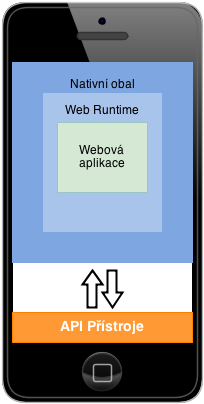
\includegraphics[width=0.4\textwidth]{hybrid_app_architecture.png}
\caption{Struktura hybridní aplikace \cite{ibm_worklight_overview}}
\label{fig:HybridAppArchitecture}
\end{figure} 

Pojďme si nyní detailněji popsat jednotlivé části. Samotná webová aplikace nemá zcela obvyklou strukturu, na kterou jsme zvyklí z tvorby klasických webových stránek. Velice často jde o jediný HTML soubor, kde je uvnitř elementu <body> ukryta celá architektura aplikace. Tento přístup umožňuje použití některého z oblíbených JavaScriptových frameworků, jako je např. jQuery Mobile, Zepto JS nebo Sencha Touch. Struktura samotné stránky pak vypadá nějak takto:


\begin{lstlisting}[language=HTML,breaklines=true]

<body>
<!-- Start of first page -->
<div data-role="page" id="foo">
  <div data-role="header">
    <h1>Foo</h1>
  </div><!-- /header -->

  <div data-role="content">
    <p>I'm first in the source order so I'm shown as the page.</p>
    <p>View internal page called <a href="#bar">bar</a></p>
  </div><!-- /content -->

  <div data-role="footer">
    <h4>Page Footer</h4>
  </div><!-- /footer -->
</div><!-- /page -->

<!-- Start of second page -->
<div data-role="page" id="bar">
  <div data-role="header">
    <h1>Bar</h1>
  </div><!-- /header -->

  <div data-role="content">
    <p>I'm the second in the source order so I'm hidden when the page loads.I'm just shown if a link that references my id is beeing clicked.</p>
    <p><a href="#foo">Back to foo</a></p>
  </div><!-- /content -->

  <div data-role="footer">
    <h4>Page Footer</h4>
  </div><!-- /footer -->
</div><!-- /page -->
</body>
\end{lstlisting}

Samotné přechody mezi stránkami jsou realizovány buď pomocí JavaScriptu funkcemi hide() a show() či využitím přechodů definovaných ve standardu CSS3. Výše zmíněné javascriptové frameworky většinou poskytují i CSS šablonu, ve které jsou definovány styly pro různé ovládací prvky, jakými jsou například tlačítka přívětivá pro dotyk. Vývojář si pak může tyto šablony přizpůsobit k obrazu svému přidáním vlastních pravidel.

Srdcem každé hybridní aplikace je však jeho javascriptový kód, ve kterém je definována celá aplikační logika. Pro její definování je často využíván právě framework jQuery, který zjednodušuje a urychluje používání některých oblíbených javascriptových funkcí. V JavaScriptu jsou definovány všechny reakce na události, uživatelské vstupy a výpočty na pozadí.

Abychom mohli HTML zobrazit uživateli, potřebujeme webový runtime, který bude umět náš kód zobrazit a průběžně vyhodnocovat. Většinou se jedná o osekané jádro webového prohlížeče, který je jinak v systému standardně přítomen. Právě v těch omezeních je však často skrytý zádrhel pro vývojáře. Například platforma iOS používá jako runtime UIWebView, jenž má narozdíl od mobilního prohlížeče Safari značnou nevýhodu v absenci javascriptového enginu Nitro, který je díky Just In Time kompilace velmi rychlý. V praxi to znamená, že pokud vaše hybridní aplikace používá JavaScript, bude UI [c]působit na uživatele pomaleji než identické UI spuštěné v prohlížeči Safari na tom samém zařízení. \cite{primer_on_hybrid_apps} Některé statistiky uvádějí, že javascriptový engine Nitro, který Safari používá, je více než 3x rychlejší než engine používaný v UIWebView. \cite{ios_for_html5_developer} Bohužel pro vývojáře není jiná možnost, jak toto omezení obejít, než používat co nejméně JavaScriptu je možné a pokoušet se ho nahradit například CSS3. Což je pro hybridní aplikace životně závisející na JavaScriptu velký problém.

Webový runtime není v podstatě ničím jiným než obyčejným objektem, který v sobě ukrývá renderovací jádro (např. WebKit). Původním smyslem tohoto objektu bylo dát možnost vykreslovat HTML obsah uživatelům v rámci nativních aplikací. Například Twitter ve své oficiální aplikaci používá takový webový runtime pro otevírání odkazů z tweetů. Uživateli se tak zobrazil obsah odkazu přímo v rámci aplikace a nemusel přepínat mezi aplikací a prohlížečem.

Tvůrcům hybridních frameworků se však podařilo uzpůsobit tyto objekty tak, aby se daly použít jako wrapper pro webovou aplikaci. Tohoto uzpůsobení je dosaženo pomocí rozšíření originálních tříd (UIWebView respektive WebView) v nativním kódu. Objekty jsou obohaceny o množství funkcí, které přispívají k optimálnímu běhu hybridní aplikace pomocí specifických reakcí na rozličné události.

Nyní, když chápeme jak funguje webový runtime, si můžeme vysvětlit jak probíhá komunikace mezi webovou aplikací a nativními funkcemi telefonu. Tato komunikace může probíhat v zásadě dvěma způsoby:

\begin{enumerate}
	\item Přímo z HTML pomocí HTML5 API.
	\item Pomocí volání konkrétních javascriptových funkcí dle specifikace konkrétního frameworku.
\end{enumerate}

Na prvním způsobu není nic zvláštního. V dnešní době jej mohou využívat i moderní webové stránky, pokud si je uživatel zobrazí v některém z novějších prohlížečů, jenž implementuje konkrétní funkci z HTML5 standardu. Všeobecně rozšířeným API voláním, které je možno volat přímo z HTML, je například geolokace nebo úložiště pro lokální ukládání dat. Tato volání vyhodnotí přímo webový runtime a sám se postará o zavolání konkrétní nativní funkce vhodné pro splnění požadavku.

\begin{figure}\centering
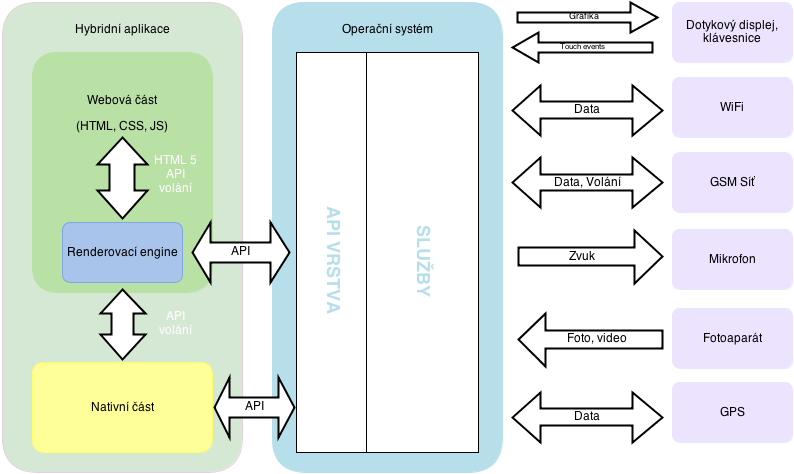
\includegraphics[width=1.0\textwidth]{hybridni_aplikace_komunikace.png}
\caption{Komunikace hybridní aplikace s operačním systémem}
\label{fig:HybridAppCommunication}
\end{figure} 

Větší pozornost si zaslouží druhý způsob komunikace s nativními funkcemi. Při něm již využijeme tzv. nativního mostu, který nám poskytuje samotný hybridní framework. Jedná se zpravidla o sadu tříd napsanou v nativním jazyce dané platformy, které slouží k zprostředkovávání komunikace mezi javascriptovými funkcemi definovanými v samotné webové aplikaci a operačním systémem zařízení, na kterém hybridní aplikace běží. V rámci každého operačního systému je třeba tento most implementovat odlišně. Každá platforma totiž umožňuje nějakým způsobem komunikovat mezi webovým runtimem a operačním systémem. Úkolem pro tvůrce hybridních frameworků je přijít s řešením, kterak zprostředkovat vývojáři sadu funkcí, které nezávisle na platformě poskytují aplikaci stejné služby a přitom nedat znát, že „za oponou“ probíhají zásadně odlišné procesy. Právě tato funkcionalita je klíčem k multiplatformnosti hybridních aplikací.

Logickým faktem je, že tzv. nativní most musí fungovat oboustranně, tj. nejen zpracovávat požadavky od webové aplikace, ale zároveň být schopen vrátit odpověď od operačního systému aplikaci zpět. Ač to zní jako poměrně triviální logika, každá z těchto cest je obvykle implementována velmi odlišně. Jak jsme již zmínil, implementace tohoto nativního mostu se může lišit framework od frameworku, já v rámci této sekce popíši, jak tento most funguje v nejpoužívanějším hybridním frameworku PhoneGap.

Ve PhoneGap je most mezi JavaScriptem a operačním systémem (v tomto případě Android) realizován pomocí Promptu. JavaScriptová API volání (například kamera, mikrofon apod.) jsou konvertována jako prompt příkaz, který je odposlechnut funkcí onJsPrompt definované webovým runtimem, která příkaz rozpozná a provede odpovídající nativní volání. \cite{dissecting_phonegap_architecture} 

Opačná cesta je realizována poněkud méně elegantním způsobem. Funguje na principu neustálého dotazování se nativní strany na odpověď. Aplikační strana se v intervalu 50 milisekund ptá nativní strany, zdali už je připravená odpověď na vznesený dotaz. Pokud je odpověď pozitivní, most zprostředkuje příchozí data klientské aplikaci.

V rámci operačního systému iOS vypadá schéma komunikace poněkud jednodušeji. V iOS funguje nativní most pro komunikaci směrem z klientské aplikace na principu iFrame, kdy jsou javascriptová volání nativních funkcí skladována ve frontě, ze které jsou následně čtena a prováděna pomocí nativní komponenty. Alternativou k tomuto přístupu je použití XHR dotazů. Klientská strana provede XHR dotaz na falešnou URL adresu v níž jsou umístěné příkazy, které se mají provést. Tyto příkazy jsou odposlechnuty, seřazeny a následně vykonány nativní stranou. \cite{dissecting_phonegap_architecture}

I komunikace opačným směrem je realizována poněkud jednodušeji, než je tomu u operačního systému Android. V iOS je veškerá zpětná komunikace prováděna pomocí funkce stringByEvaluatingJavaScriptFromString zprostředkované webovým runtimem UIWebView. \cite{dissecting_phonegap_architecture}

\section{Příklady hybridních frameworků}
\subsection{PhoneGap}
Vzhledem k tomu, že hybridnímu frameworku PhoneGap je věnována celá následující kapitola, zmíním ho zde opravdu jen velmi stručně.

PhoneGap je framework vlastněný a vyvíjený společností Adobe. Jedná se o zdaleka nejpopulárnější řešení na poli hybridních frameworků, což dokládá i fakt, že řada dalších hybridních frameworků na PhoneGapu staví a začleňuje jej do vlastních řešení.

PhoneGap v současné době oficiálně podporuje 7 mobilních platforem. V době psaní této bakalářské práce PhoneGap pokrýval 17 nativních API volání. Mezi ty nejpoužívanější dozajista patří geolokace, přístup k filesystému, fotoaparát či akcelerometr. Všechna API volání si podrobněji popíšeme v další kapitole spolu s detailním popisem celého frameworku PhoneGap.

\subsection{Sencha Touch}
Zařazení produktu Sencha Touch mezi hybridní frameworky je možná trochu odvážné. Já se toho přesto dopustím, protože Sencha Touch ve svých nejnovějších verzích poskytuje nástroje pro tvorbu hybridních aplikací, ač je jinak stále dominantně UI frameworkem.

Sencha Touch má za sebou již tři roky vývoje. Jejím primárním úkolem vždy bylo poskytovat vývojářům možnost rychle vyvíjet uživatelské rozhraní mobilních webových aplikací optimalizované pro použití na zařízeních s dotykovým displejem. Neméně důležité však je, aby zobrazované rozhraní vypadalo na dané platformě co možná nejvěrněji. V tomto přístupu se tedy příliš neliší od frameworku jQuery Mobile a dá se říci, že na poli javascriptových frameworků jsou právě jQuery Mobile a Sencha Touch těmi největšími konkurenty.

Hlavním posláním těchto UI frameworků je poskytnout vývojáři sadu vizuálních elementů jako jsou tlačítka, toolbary, seznamy, pop-up okna, formuláře, textová pole, přechody mezi stránkami atp., které mohou použít ve svých aplikacích, aniž by museli složitě pomocí CSS a JavaScriptu definovat tyto elementy sami. Zároveň jsou tyto vizuální prvky optimalizovány k maximální kompatibilitě a výkonu na co možná nejširším portfoliu webových prohlížečů.

Sencha v současné době podporuje 4 platformy (iOS, Android, Blackberry a Windows Phone 8). Použití tohoto produktu je pro většinu účelů zdarma, platit musíte jen pokud chcete na jeho základě postavit vlastní komerční framework.

Nyní si pojďme osvětlit, proč zařazuji Sencha Touch mezi hybridní frameworky. Vývojáři tohoto produktu totiž do jeho druhé verze přidali (v rámci nástroje Sencha Touch Preview SDK Tools) možnost přístupu k některým nativním API voláním mobilních platforem. Nabízejí také možnost zabalení webové aplikace do nativních binárních souborů vhodných k publikaci na oficiálních tržištích jednotlivých mobilních platforem. Sluší se dodat, že celá tato funkcionalita je stále značně omezená, protože podporovány jsou pouze dvě platformy (iOS a Android) a dostupné jsou pouze 4 API volání (indikace připojení k internetu, nativní notifikace, orientace zařízení a přístup k fotoaparátu). Dá se však očekávat, že se vývojáři pracující na frameworku Sencha Touch budou snažit dále rozšiřovat tento nástroj, aby podporoval více API volání a více platforem.

\subsection{MoSync Wormhole}
MoSync je velice zajímavý framework, který pokračuje de facto tam, kde PhoneGap končí. Nejedná se o klasický hybridní framework, neboť možnosti jeho využití jsou mnohem širší a hybridní funkcionalita do něj byla přidána až relativně nedávno.

Prapůvodním důvodem vzniku MoSync frameworku bylo umožnit vývojářům, kteří ovládají jazyky C nebo C++, vyvíjet nativní mobilní aplikace bez nutnosti měnit své programovací návyky a zároveň jim dát možnost zasáhnout více platforem najednou. Později byla přidána možnost vytvářet webové aplikace s využitím HTML5 a také hybridní aplikace s využitím obojího: HTML5 i nativního mostu napsaného v C/C++.

Vývojářům je tedy umožněno vytvářet klasické hybridní aplikace, ve kterých mohou přistupovat k nativním funkcím telefonu (geolokace, fotoaparát, filesystém apod.) a finální aplikace zabalit do nativních balíčků připravených na distribuci na oficiální tržiště. V současné době jsou pro hybridní účely podporovány tři hlavní platformy iOS, Android a Windows Phone[e].

\begin{figure}\centering
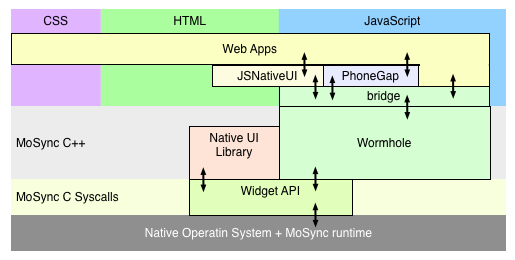
\includegraphics[width=1.0\textwidth]{MoSyncUI_Layers.png}
\caption{Architektura frameworku MoSync Wormhole \cite{javascript_for_native_widgets}}
\label{fig:MoSyncWormholeArchitecture}
\end{figure} 

Na obrázku \ref{fig:MoSyncWormholeArchitecture} můžeme vidět, jak funguje komunikace mezi webovou aplikací a nativním operačním systémem.

Celá tato hybridní technologie se nazývá Wormhole a její javascriptová část implementuje některé technologie z frameworku PhoneGap stejně jako některé novinky z HTML5 standardu (například geolokace). Velkou výhodou, kterou MoSync oproti PhoneGap nabízí, je možnost využít ve své aplikaci nativní UI elementy jako jsou tlačítka, různé lišty atp. To může být pro vývojáře skutečně zajímavé, protože bude využívat pravé nativní prvky místo často těžkopádných (v CSS emulovaných) náhražek. Tato technologie je však logicky úkrokem stranou od klasických wrapperů, které balí webové aplikace do webového runtimu. Jelikož webový runtime neumí vykreslovat nativní elementy, je pro tyto účely využit MoSync runtime, který pracuje s hybridní aplikací na podobném principu jako framework Titanium zmíněný ve třetí kapitole.

Fakt, že MoSync implementuje funkcionalitu z frameworku PhoneGap dodává tomuto nástroji další přidanou hodnotu. Většina aplikací napsaná ve PhoneGap je s MoSync kompatibilní a tak mohou vývojáři bezbolestně rozšířit své PhoneGap aplikace o nativní UI elementy, které poskytuje nástroj MoSync.

Framework MoSync je open-source a je šířen zdarma.

\subsection{IBM Worklight}
Worklight je vývojová platforma vyvíjená pod záštitou technologického giganta IBM. Umožňuje vývoj nativních, webových i hybridních aplikací. Tato platforma může být zajímavá zejména pro využití ve firmách, neboť pro enterprise účely přináší několik zajímavých nástrojů.

\paragraph{IBM Worklight umožňuje vyvíjet hybridní aplikace třemi způsoby \cite{ibm_worklight_overview}:}
\begin{enumerate}
	\item Vývoj klasické hybridní aplikace. Z vašeho javacriptového kódu voláte funkce operačního systému přes nativní most, který zajišťuje nástroj PhoneGap. Jedná se tedy o identický přístup, který používá většina hybridních frameworků.
	\item Vývoj částečně nativní aplikace. Vývojář může ve své aplikace využít zmenšeného web view a zbytek UI implementovat pomocí nativních UI komponent.
	\item Vývoj částečně hybridní aplikace. Uživatelé vyvíjejí kompletní uživatelské rozhraní pomocí nativních jazyků, ale pokud je to potřeba, mohou využívat i web views s hybridní funkcionalitou.
\end{enumerate}

IBM Worklight je celá sada nástrojů pro vývoj mobilních aplikací. Základem je IBM Worklight Studio – IDE postavené na open-source platformě Eclipse, které krom klasických funkcí nabízí i možnost tvorby uživatelského rozhraní pomocí WYSIWYG editoru. Vývojář si pomocí funkce drag \& drop přetahuje jednotlivé UI elementy (podporovány jsou HTML5, jQuery Mobile a Dojo Mobile) a modeluje si tím vzhled své aplikace.

Dalším užitečným nástrojem je IBM Worklight Server, který slouží jako middleware mezi uživatelskými aplikacemi a různými back-endovými systémy či cloudovými službami. Tato služba také řídí veškerý vzdálený přístup k aplikaci. Pro firemní účely dále obsahuje platforma Worklight nástroje jako jsou  IBM Worklight Application Centre, IBM Worklight Centre a IBM Worklight Device Runtime Components, které slouží ke vzdálené správě (přístup, push notifikace, analýza používání atd.) či distribuci (oficiální či privátní tržiště) aplikací.

\subsection{FeedHenry}
FeedHenry je společnost stojící za nástrojem Mobile Application Platform. Tato platforma je určena především pro enterprise segment trhu. Pro tvorbu hybridních aplikací je využíván PhoneGap, který zajišťuje propojení webové a nativní části.

Mobile Application Platform se zaměřuje především na pohodlné napojení aplikace na firemní back-end systémy a také na bezpečnost finálních aplikací, což jsou v korporátním prostředí vyhledávané benefity. FeedHenry dále poskytuje nástroje pro správu a analýzu aplikací v cloudu. Umožňuje jednoduché odeslání aplikací na privátní firemní tržiště, kde mohou firmy publikovat aplikace pro své zaměstnance či klienty.

\subsection{Icenium}
Icenium je, co se uživatelského přístupu týká, velmi inovativní nástroj. Veškerý vývoj totiž přesunul do cloudu. Nemusíte si stahovat žádné IDE či SDK. Pouze se zaregistrujete a vyvíjíte hybridní aplikace přímo v prohlížeči. Váš kód je umístěn buď ve verzovacím systému, který poskytuje samotný framework nebo můžete využít nástroje Git.

V cloudu se nachází i SDK jednotlivých platforem (v současnosti jsou podporovány pouze iOS a Android) a také knihovny nástroje Apache Cordova (PhoneGap), jehož služeb Icenium využívá. Krom vývojového prostředí se v cloudu nachází také testovací nástroje, které vývojářům umožňují real-time zobrazení uživatelského rozhraní a otestování funkčnosti samotné aplikace.

\subsection{WYSIWYG frameworky s využitím PhoneGap}
Do této skupiny řadím sobě podobné frameworky jako jsou například ApplicationCraft či Tiggzi, které vykazují společné znaky zejména v tom, že využívají pro tvorbu hybridních aplikací technologii z frameworku PhoneGap a zároveň jako primární způsob vývoje nabízí vývojářům v cloudu integrované WYSIWYG nástroje, kde je tvorba aplikací realizována pomocí mechanismu drag \& drop. Vývojář (nebo spíše modelář) aplikace skládá jednotlivé vizuální či funkční elementy a postupně tak vytváří svojí aplikaci. Díky využití PhoneGap může přistupovat k nativním funkcím operačního systému a následně hotovou aplikaci zabalit do nativního balíčku a distribuovat na oficiální tržiště.

\subsection{Srovnávací tabulka}
V následující tabulce naleznete přehledné porovnání jednotlivých hybridních frameworků dle následujících kritérií:

\begin{enumerate}
	\item Podporované platformy
	\item Podporovaná nativní API volání
	\item Poskytnutí vlastního IDE
	\item Licence a cena
\end{enumerate}

% TODO tabulka

% Kapitola PhoneGap
\chapter{PhoneGap}
	\section{Obecně}
Jak již bylo v textu této práce několikrát zmíněno, PhoneGap je v současné době pravděpodobně nejpoužívanější a nejznámější hybridní framework. Vývojáři se na svém webu chlubí, že zaznamenali již více než milion stažení jejich produktu a zároveň tvrdí, že je v současné době používán více než 400 000 vývojáři pro tvorbu tisícovek aplikací.

PhoneGap umožňuje vývojářům využívat při tvorbě mobilních aplikací webové technologie HTML5, CSS3 a JavaScript a zároveň jim prostřednictvím vlastního javascriptového API poskytuje možnost komunikace s operačním systémem a využití jeho nativních součástí, jako je například fotoaparát, akcelerometr nebo například výběr ze seznamu kontaktů. To vše multiplatformně.

V rámci této kapitoly již nebudu zabíhat do technických detailů vlastního fungování frameworku PhoneGap. Tuto oblast jsem již dostatečně pokryl v předchozí kapitole \ref{Chap:HybridniFrameworky}.

„The ultimate purpose of PhoneGap is to cease to exist.“ \cite{how_cordova_becomes_phonegap}

Skupina vývojářů stojící za PhoneGap uvádí, že za jejich prací stojí následující dvě kréda:

\begin{enumerate}
	\item Web vyřešil problém přenositelnosti.
	\item Každá technologie zastará.
\end{enumerate}

S prvním krédem se dá polemizovat jen velmi těžko. Program, umožňující zobrazovat webové stránky, najdeme dnes skutečně téměř na každé platformě. Co se ne zcela povedlo Javě, se webovým technologiím daří a jejich význam roste. Ne náhodou dnes používáme mnohem více webových aplikací než dříve a spousta aplikací, u kterých to bylo dříve nemyslitelné, se přesunula do cloudu a přistupujeme k nim přes webový prohlížeč. Jedním z nejzářnějších příkladů jsou například Google Dokumenty, které přispěly i k tvorbě této práce.

Krom těchto dvou kréd uvádějí vývojáři i dva cíle, ke kterým by jejich snažení mělo přispět:

\begin{enumerate}
	\item Vylepšit web (webové standardy), aby se stal prvotřídní vývojovou platformou.
	\item Docílit takového stavu webových standardů, aby byl PhoneGap zbytečný.
\end{enumerate}

Je pravdou, že různé týmy uvnitř konsorcia W3C pracují na vytvoření standardů, které umožní přístup k nativním funkcím telefonního přístroje přímo z prohlížeče bez použití jakékoliv mezivrstvy. Typickým příkladem realizace těchto snah je například standard pro využití geolokace, který již byl moderními prohlížeči implementován a je využit i v rámci PhoneGap, kde API volání pro geolokaci nedělá nic jiného, než že volá tuto standardizovanou funkci prohlížeče. Že cíle, které si tým kolem PhoneGap vytyčil, nejsou řečmi do větru, dokládá i fakt, že vývojáři stojící za tímto frameworkem jsou součástí právě těch skupin v rámci konsorcia W3C, které se starají o implementaci příslušných standardů.

\subsection{Licence}
Poté co byla firma Nitobi, která za PhoneGap původně stála, odkoupena společností Adobe, byl kód pohánějící framework PhoneGap věnován organizaci Apache Software Foundation pod názvem Apache Cordova. Nyní je tedy šířen pod licencí Apache License, Version 2. Tato licence nadále zaručuje otevřený přístup k vývoji na projektu i k použití samotného kódu.

\subsection{PhoneGap vs. Apache Cordova}
Zejména u lidí, kteří se s PhoneGap teprve seznamují, koluje mnoho nejasností ohledně rozdílu mezi PhoneGap a jeho dvojčetem Apache Cordova. Myslím, že stojí za to na tomto místě tyto nejasnosti ozřejmit.

Apache Cordova je jádro frameworku spravované Apache Software Foundation (ASF), na jehož základě je postavený framework PhoneGap. Dalo by se říci, že PhoneGap je distribucí Apache Cordova podobně, jako je operační systém Ubuntu distribucí, kterou pohání jádro Linux. Vývojáři PhoneGap nadále doplňují Apache Cordova o nové funkce a opravují nalezené chyby. K oddělení došlo zejména proto, že postupem času se dá očekávat hlubší integrace PhoneGap s nástroji Adobe, což by nebylo vhodné pro masové použití \cite{cordova_name}. 

PhoneGap není jedinou distribucí Apache Cordova, ve skutečnosti jí dnes implementuje do svých nástrojů mnoho firem, jako je například Salesforce nebo Facebook \cite{cordova_name}. Na vývoji Apache Cordova se nepodílí jen vývojáři PhoneGap, ale také mnoho dalších firem jako je například IBM či Microsoft.

\section{Historie}
„We went down with one goal in mind and that was to make native iPhone features available to web apps.“ \cite{phonegap_announcement}

Pojďme se stručně seznámit s historií PhoneGap a změnami, které vedly k frameworku, jak jej známe dnes. PhoneGap vznikl v roce 2008 na vývojářské akci iPhoneDevCamp, kde vývojáři firmy Nitobi přišli s nápadem, kterak umožnit vývojářům webových aplikací pro systém iOS (tehdy ještě iPhone OS) využívat některé oblíbené nativní funkce přístroje iPhone. V soutěži na iPhoneDevCamp sice PhoneGap neuspěl, to však firmu Nitobi nezastavilo v dalším rozvíjení svého nápadu.

V počátku své existence podporoval PhoneGap pouze systém iOS, ale multiplatformnost byla brána vývojáři na zřetel od samého počátku, a tak rychle přibyla podpora pro Android a BlackBerry. Nedlouho poté (v roce 2009) následovala podpora pro Symbian a Palm (webOS).

K začátkům frameworku PhoneGap se datuje série nepříjemností, které vznikly při schvalovacím procesu ze strany Applu, kdy Apple odmítal schvalovat a vpouštět na své oficiální tržiště aplikace napsané pomocí frameworku PhoneGap. Důvodem pro zamítání aplikací bylo porušení podmínek, které aplikace v AppStore musí splňovat. Aplikace napsané ve PhoneGap byly penalizovány, protože při jejich vývoji byl použit externí framework, což tyto podmínky zapovídají. Celá záležitost byla vyřešena domlouvou mezi vývojáři kolem frameworku PhoneGap a Applem, kdy byla stanovena „bezpečná verze“ frameworku PhoneGap (PhoneGap 0.8.0), jejíž použití bylo Applem oficiálně posvěceno a k aplikacím využívajícím tuto „bezpečnou verzi“ bylo během schvalovacího procestu přistupováno stejně jako k běžným nativním aplikacím. \cite{open_letter_to_apple} + \cite{updates_on_apple} + \cite{phonegap_permitted_appstore} + \cite{phonegap_store_approval}

Multiplatformní záběr se stal zas o něco širším, když v roce 2010 přidal PhoneGap podporu pro Windows Phone 7 a také kvůli přechodu BlackBerry na WebKit, v šesté verzi svého operačního systému, byla podpora pro BlackBerry rozštěpena na dvě větve.

V listopadu 2010 Nitobi představilo v poloveřejné betě nástroj PhoneGap Build. Tento nástroj si podrobněji popíšeme později v této kapitole, teď jen zmíním, že se jedná o cloudovou službu, která umožňuje po nahrání zdrojových kódu vygenerovat instalační balíčky pro více platforem najednou. Vývojář tak nemusí pro každou platformu instalovat její SDK a generování binárek provádět ručně \cite{announcing_phonegap_build_beta}. 

Pokračující růst PhoneGap dokládá i obliba, které se této framework těšil pouhé dva roky po svém vzniku. V listopadu 2010 zaznamenal PhoneGap již 350 000 stažení. S touto vzrůstající oblibou začalo Nitobi (původně konzultantská firma zabývající se tvorbou webů a javascriptových knihoven) na PhoneGap stále více sázet ve své obchodní strategii. Nejenže s ním pracovala ve své konzultantské činosti a doporučovala jeho používání svým zákazníkům, ale v únoru 2011 zavádí i placenou podporu pro vývojáře ve PhoneGap, v rámci které jim poskytuje webináře, přístup na privátní forum a pomoc v rámci office hours.

Dalším znakem úspěchu PhoneGap je i jeho adopce softwarovými giganty jako je Adobe či IBM, které začali tento framework integrovat do svých nástrojů, jako je Adobe DreamWeaver či IBM Worklight \cite{phonegap_worklight_enterprise} + \cite{dreamweaver_supports_phonegap}. 

Prvním velkým milníkem pro PhoneGap bylo vydání verze 1.0.0, ke kterému došlo 29. 7. 2011 \cite{phonegap_1_released}. V té době PhoneGap již podporoval i platformu Samsung Bada a samotný framework zaznamenal 600 000 stažení s průměrem kolem 40 000 stažení měsíčně \cite{phonegap_1_released}. 

V září 2011 se PhoneGap Build přesouvá do veřejné betaverze a zároveň byly zveřejněny cenové plány pro jeho použití. Ty se pohybovali od \$0 pro vývoj open-source aplikací po \$900 ročně pro vývoj komerčních aplikací s uzavřeným kódem. \cite{phonegap_build_open_beta}

3. září 2011 Nitobi na svém blogu oznámilo, že uzavřelo dohodu o svém převzetí firmou Adobe \cite{nitobi_adobe1}.

“PhoneGap has proven to be an industry-defining app solution for HTML5 developers,” said Danny Winokur, vice president and general manager, Platform, Adobe \cite{nitobi_adobe1}.

"It’s a perfect complement to Adobe’s broad family of developer solutions, including Adobe AIR, and will allow us to continue to provide content publishers and developers with the best, cutting-edge solutions for creating innovative applications across platforms and devices.” \cite{nitobi_adobe1}

V rámci tohoto převzetí Nitobi oznámilo, že věnuje zdrojové kódy frameworku PhoneGap organizaci Apache Software Foundation (ASF) pod názvem Apache Callback, který byl později změněn na Apache Cordova \cite{nitobi_adobe2} + \cite{phonegap_13_released}. 

Akvizice Nitobi firmou Adobe se podařila úspěšně dokončit 27. října 2011 \cite{nitobi_adobe2}. Analytici se shodují, že hlavním smyslem této akvizice byla snaha Adobe posílit svojí pozici na poli vývoje aplikací v HTML5, protože jeho vlastní technologie Flash je (zvlášť v mobilním světě) na ústupu. Očekávalo se začlenění PhoneGap do vývojářských nástrojů, které Adobe poskytuje webovým vývojářům.

Nehledě na tuto velkou změnu popularita PhoneGap dále pozvolna stoupala a v červnu roku 2012 dosahoval průměrný měsíční počet stažení hodnoty 100 000 \cite{phonegap_myths}.

20. července 2012 byla oficiálně uvolněna verze 2.0, která (krom jiného) přinášela také Cordova WebView, což je možnost použití WebView v rámci nativní aplikace současně se všemi výhodami PhoneGap. Dále přibylo také mnoho vylepšení command-line interfacu, které umožňuje ovládat PhoneGap z konsole \cite{phonegap_2_released}. 

V září 2012 byl oficiálně spuštěn PhoneGap Build, který je nyní dostupný ve stabilní verzi \cite{phonegap_build_launched}. Zároveň byla v listopadu 2012 vydána verze 2.2.0, která přináší podporu Windows 8 v rámci PhoneGap. V době psaní této práce se framework nachází ve verzi 2.5.0. Vydání verze 3.0.0 je naplánováno na červenec 2013 \cite{cordova_roadmapprojects}. 

\subsection{Ocenění}
PhoneGap se za dobu své existence dočkal celé řady ocenění od všemožných institucí.

\begin{enumerate}
	\item 2009: People’s Choice award v rámci Web 2.0 Expo LaunchPad competition \cite{phonegap_winning_webexpo}. 
	\item 2012: Best Cross-Platform Development Tool by CodeProject \cite{phonegap_best_xplatfrom_tool}
	\item 2012: Technology of the Year By InfoWorld \cite{infoworld_technology_of_2012}
	\item 2012: “Champion” by Info-Tech Research Group v rámci 2012 Vendor Landscape: Mobile Development Platforms \cite{phonegap_champion}
	\item 2012: Best Mobile Development Tool by Dr. Dobb's Jolt Awards \cite{phonegap_best_mobile_dev_tool}
\end{enumerate}

\section{Vývojářské nástroje}
\subsection{Vývoj}
Na začátku této sekce krátce pohovořím o nástrojích, které můžeme pro vývoj ve PhoneGap využít. Před vznikem cloudové služby PhoneGap Build byl vývoj, zvláště pokud jste chtěli aplikaci cílit na více platforem, poměrně kostrbatý. To bylo zapříčiněno několika faktory:

\begin{enumerate}
	\item Různá SDK pro sestavení nativních binárek
	\item Různá adresářová struktura projektů pro jednotlivé platformy
	\item Odlišné javascriptové knihovny (PhoneGap) pro jednotlivé platformy
\end{enumerate}

V důsledku to znamenalo, že pro vývoj aplikace pro systém Android jste si museli stáhnout Eclipse a Android SDK a vývoj vést v těchto nástrojích. Pokud jste následně chtěli aplikaci portovat na iOS, znamenalo to stažení iOS SDK a Xcode (funguje pouze na systému Mac OS), úpravu adresářové struktury projektu a využití knihovny PhoneGap určené pro systém iOS.

Díky cloudovému nástroji PhoneGap Build (podrobněji si ho popíšeme níže v této kapitole) se vývoj aplikací ve PhoneGap výrazně usnadnil a to zejména při cílení na více platforem. Jelikož PhoneGap Build potřebuje k vygenerování nativních binárek pouze samotné zdrojové kódy aplikace, nemusí se vývojář zabývat ani jedním z výše vyjmenovaných problémů.

Pokud vývojář není závislý na SDK konkrétní platformy, může pro vývoj použít prakticky libovolný nástroj. Může zůstat u mohutného IDE, jako je např. Eclipse nebo využít svůj oblíbený textový editor (TextMate, gedit, Sublime Text apod.).

\subsubsection{Hello World}
Pojďme si ukázat, jak se PhoneGap inicializuje. Ukážeme si to na příkladu klasické Hello World aplikace:

\begin{lstlisting}[language=HTML,breaklines=true]
<!DOCTYPE html>
<html>
  <head>
      <meta http-equiv="Content-Type" content="text/html; charset=UTF-8" />
      <meta name="viewport" content="user-scalable=no, initial-scale=1, maximum-scale=1, minimum-scale=1, width=device-width, height=device-height, target-densitydpi=device-dpi" />
<!-- INCLUDE CORDOVA -->
        <script type="text/javascript" src="cordova-2.4.0.js"></script>
<script type="text/javascript">
        // Wait for Cordova to load
            function onBodyLoad() {
                    document.addEventListener("deviceready", onDeviceReady, false);
            }
            
            // Cordova is ready
            function onDeviceReady() {
        navigator.notification.alert("PhoneGap is ready!");
}
</script>
<body onload="onBodyLoad()">
        <h1>Hello World!</h1>
        <p>This is a sample PhoneGap application.</p>
  </body>
</html>
\end{lstlisting}

K inicializaci frameworku PhoneGap v tomto případě dojde v několika krocích. Jednak samotné vložení knihovny “cordova-2.4.0.js” do hlavičky HTML dokumentu. Dalším krokem je vytvoření funkcí onBodyLoad() a onDeviceReady(). V rámci funkce onBodyLoad() čekáme, až PhoneGap provede veškerou inicializaci svých součástí. Jakmile se to stane, je zavolána funkce onDeviceReady(), kde provedeme zavolání funkce navigator.notification.alert(), která je definována v API frameworku PhoneGap a liší se od klasické javascriptové funkce alert(). Funkce onBodyLoad() a onDeviceReady() jsou nedílnou součástí víceméně každé aplikace napsané ve frameworku PhoneGap.

Abych demonstroval, jak jednoduché je zavolání některého z javascriptových API nabízených frameworkem PhoneGap, ukáži, jak by vypadala funkce, kterou bychom mohli vytvořit pro pořízení fotografie prostřednictvím fotoaparátu.

\begin{lstlisting}[language=HTML,breaklines=true]
<!-- Vyfot fotku a vrat ji jako URI -->
function takePhoto() {
navigator.camera.getPicture(photoSuccess, photoFail, {quality: 50,
                            destinationType: Camera.DestinationType.FILE_URI});
  }
\end{lstlisting}

V případě úspěchu je zavolána funkce photoSuccess, kde můžeme fotografii dále zpracovat. V opačném případě je zavolána funkce photoFail, kde můžeme například vypsat uživateli zprávu o chybě.

Jednotlivá API volání, které framework PhoneGap nabízí, si podrobněji popíšeme v podkapitole \ref{Sec:API}.

\subsection{Rozšíření}
Pokud vyvíjíme pro konkrétní platformu nebo chceme jen přidat některé specifické funkce, které PhoneGap nativně nenabízí, můžeme sáhnout do poměrně bohaté sbírky rozšíření, která vznikla v rámci komunity, ale je oficiálně spravována projektem PhoneGap na adrese https://github.com/purplecabbage/phonegap-plugins. % TODO vylepšit URL

Najdeme tu bohatou sbírku pluginů, které pokrývají širokou škálu funkcí. Můžeme si některé z nich uvést:

\begin{enumerate}
	\item InAppPurchaseManager (iOS)
	\item BarcodeScanner
	\item GoogleAnalytics
	\item PDFViewer
	\item Twitter
	\item iCloudKV (iOS)
	\item Bluetooth
	\item NFC
	\item PayPalPlugin
\end{enumerate}

Pluginy se používají podobným způsobem jako samotný framework. Konkrétní plugin se vloží do projektu a jeho funkce jsou následně volány z javascriptového kódu vlastní aplikace. Logicky je nutné počítat s tím, že použití takového pluginu silně ochromí přenositelnost celé aplikace a před provedením portu bude třeba provést odpovídající úpravy.

\subsection{Debugování a testování} \label{Sec:DebugaTest}
\subsubsection{Testování}
V průběhu celého vývoje aplikace je třeba neustále testovat a ověřovat její funkčnost v prostředí co možná nejbližším produkčnímu. Pro tento účel poskytují tvůrci jednotlivých platforem simulátory (emulátory), které simulují běh aplikace v rámci daného operačního systému či dokonce přímo v rámci konkrétního zařízení.

V případě testování není žádný rozdíl mezi nativními aplikacemi a těmi hybridními napsanými ve PhoneGap. Vývojář nahraje svojí aplikaci do simulátoru a zkouší její funkčnost. To samé se týká testování aplikace na reálném zařízení, které by mělo být součástí každého vývojového plánu.

\subsubsection{Debugování}
Při vývoji čistě nativních aplikací využívá vývojář pro ladění svých aplikací debugovací nástroje, které mu poskytuje SDK a další nástroje konkrétní platformy. Problém s těmito nástroji je, že většinou nejsou připravené na ladění kódu psaného webovými jazyky. To staví vývojáře do poměrně nepříjemné pozice, kdy jsou buď nuceni protkat svůj kód voláním funkce alert() či console.log(), které používají pro vypsání ladících výpisů nebo využít některého z nástrojů třetích stran, které jsou na ladění hybridních aplikací připraveni. Dva takové nástroje si nyní uvedeme.

\paragraph{Ripple Mobile Enviroment Emulator}
Ripple Mobile Enviroment Emulator (RMEE) je náhrada klasického emulátoru z SDK jen s tím rozdílem, že je velmi odlehčený a běží jako rozšíření ve webovém prohlížeči Google Chrome či Chromium. RMEE narozdíl od holého webového prohlížeče dokáže nasimulovat i volání nativních funkcí frameworkem PhoneGap a je tak velice vhodným nástrojem pro rychlé testování mobilních aplikací bez nutnosti zdlouhavě nahrávat aplikaci do emulátoru nebo vlastního fyzického zařízení.

Výhodou použití RMEE je, že dává vývojáři k dispozici krom samotného emulátoru i veškeré vývojářské nástroje prohlížeče Google Chrome, které se používají pro ladění webových aplikací. Může tak za běhu upravovat některé parametry své aplikace a pohodlně tak ladit vlastní aplikaci.

\begin{figure}\centering
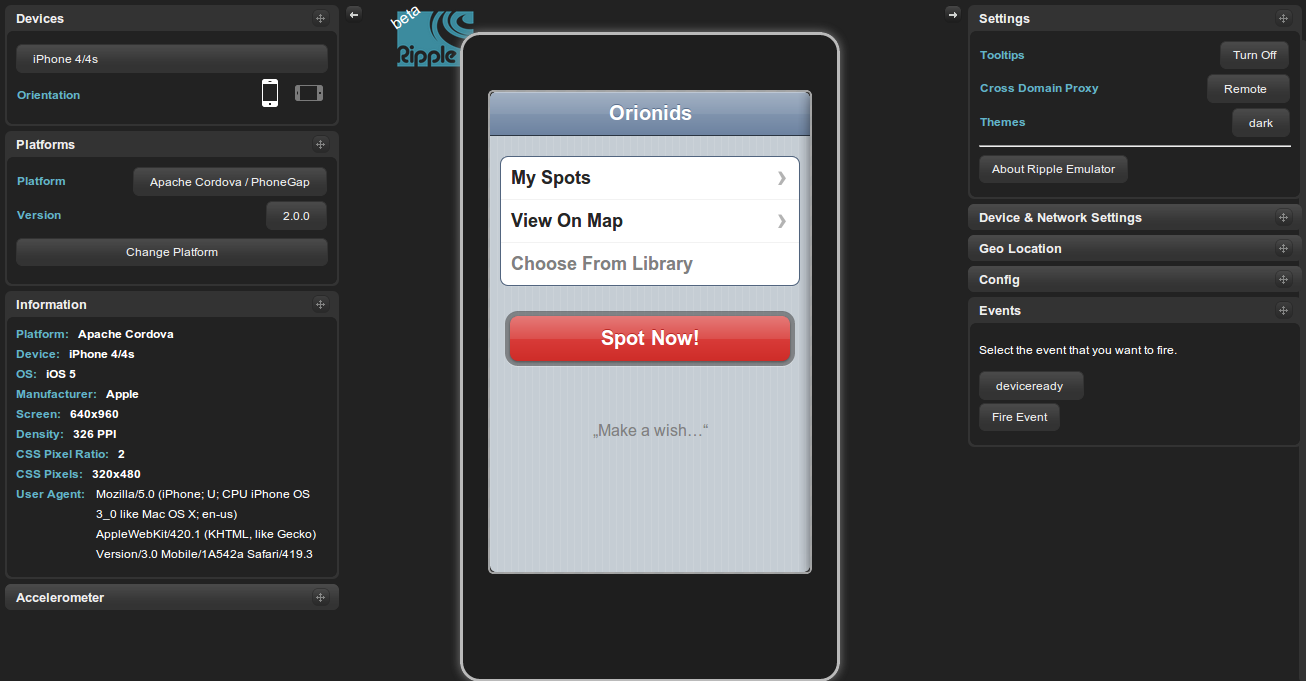
\includegraphics[width=0.9\textwidth]{RMEE.png}
\caption{Ripple Mobile Enviroment Emulator}
\label{fig:RMEE}
\end{figure} 

Je jasné, že RMEE nenahradí testování v klasickém emulátoru či dokonce na fyzickém zařízení, neboť zdaleka nedokáže emulovat veškerá specifika hostitelských operačních systémů, ale stále je poměrně vhodným nástrojem pro rychlé testování aplikace zvláště v rané fázi vývoje.

RMEE je dostupný z adresy http://emulate.phonegap.com

\paragraph{Web Inspector Remote}
Web Inspector Remote neboli Weinre je ladící nástroj trochu jiného druhu. Nezabývá se emulací běhu aplikace, ale funguje jako vzdálený ladící nástroj. Jeho použití je poměrně jednoduché. Do kódu své aplikace vložíte skript umístěný na vzdáleném serveru (http://debug.phonegap.com) s unikátním označením své aplikace.

\begin{lstlisting}[language=HTML,breaklines=true]
<script src="http://debug.phonegap.com/target/target-script-min.js#myapp"></script>
\end{lstlisting}

Samotné debugování probíhá v prohlížeči, do kterého vývojář zadá adresu serveru s identifikátorem laděné aplikace http://debug.phonegap.com/client/\#myapp. Vývojáři je k dispozici javascriptová konzole a další nástroje pro ladění webových aplikací.

\subsection{Sestavení a publikace}
Pokud již máme aplikaci vytvořenou a důkladně otestovanou, je na řadě její sestavení a případná publikace například na oficiálním tržišti s aplikacemi. Za účelem sestavení aplikace nám PhoneGap umožňuje jít dvěma cestami. První z nich je sestavení nativního instalačního balíčku s využitím SDK konkrétní platformy vhodný k odeslání na tržiště. Toto je klasická cesta a je vhodná, pokud cílíme pouze na jednu platformu. Problém nastává, pokud chceme vytvořit balíčky pro více platforem najednou. Jak jsem již zmínil výše, v takovém případě jsme nuceni stáhnout SDK každé jednotlivé platformy, náš projekt upravit a poté s pomocí SDK vytvořit nativní binárku. Že toto není dobrý způsob, si uvědomovali i tvůrci frameworku PhoneGap a proto již v počátku ve svých úvahách počítali s cloudovým nástrojem, který sestavování aplikací značně usnadní.

\subsubsection{PhoneGap Build} \label{Sec:PhoneGapBuild}
PhoneGap Build je nástroj dostupný z adresy http://build.phonegap.com. Umožňuje nám z jednoho místa a z jednoho zdrojového kódu vytvořit v jednom čase instalační balíčky pro platformy iOS, Android, Windows Phone, BlackBerry, webOS a Symbian.

Pojďme si v krátkosti popsat jak celý systém funguje. Vývojář je na začátku vyzván k propojení PhoneGap Build se svým účtem na Githubu, na němž má ve veřejném repozitáři umístěny zdrojové kódy své aplikace. Poté se dostane do ovládacího panelu, kde vybere z nabídky správný repozitář, ve kterém se PhoneGap Build pokusí najít soubor index.html. Jakmile se mu to podaří, nabídne vývojáři možnost si vygenerovat instalační balíčky pro jednotlivé platformy pomocí jednoho kliknutí. Vyhotovení balíčků trvá několik vteřin a poté jsou uživateli k dispozici ke stažení.

\section{API} \label{Sec:API}
Hlavním důvodem, proč vývojáři sahají po použití frameworku PhoneGap, je sada javascriptových API, pomocí které zprostředkovává komunikaci mezi webovou aplikací a operačním systémem na daném zařízení. Pojďme si nyní stručně popsat jednotlivá API volání.

\subsection{Accelerometer}
Akcelerometr se používá ke zjištění orientace daného přístroje. Hojně je využíván například v hrách, kde hráč ovládá hru pomocí naklopení telefonu.

\subsubsection{Metody}
\paragraph{accelerometer.getCurrentAcceleration}
Metoda vrací údaje o orientaci telefonu pomocí trojice čísel x, y a z. Každé číslo reprezentuje změnu orientace kolem jedné osy.

\paragraph{accelerometer.watchAcceleration}
Metoda umožňující neustálé sledování změn orientace v pravidelném intervalu.

\paragraph{accelerometer.clearWatch}
Umožňuje zrušit sledování změn vyvolané předchozí metodou.

\subsection{Camera}
Sada funkcí umožňující přistupovat k fotoaparátu daného zařízení.

\subsubsection{Metody}
\paragraph{camera.getPicture}
Umožňuje pořízení fotografie z daného zdroje. Zdroj je specifikován ve volání této funkce, může se jednat buď o pořízení nového snímku nebo o vybrání již pořízeného snímku z fotoalba. Fotografie je vrácena buď jako URI nebo jako String zakódovaný v base64.

\paragraph{camera.cleanUp}
Smaže dočasně uložené fotografie pořízené předchozí funkcí.

\subsection{Capture}
API umožňující zachycení videa, audia či fotografie.

\subsubsection{Metody}
\paragraph{capture.captureAudio}
Spustí výchozí aplikaci pro pořízení zvukové nahrávky a vrátí informace o pořízených záznamech (URI).

\paragraph{capture.captureImage}
Spustí aplikaci pro pořizování obrázků a vrátí informaci o zhotovené fotografii nebo fotografiích.

\paragraph{capture.captureVideo}
Spustí aplikaci pro snímání videa a vrátí informace o pořízeném klipu či klipech.

\paragraph{mediaFile.getFormatData}
Vrátí informace o formátu média.

\subsection{Compass}
Sada metod umožňující rozpoznat, jakým směrem je zařízení namířeno.

\subsubsection{Metody}
\paragraph{compass.getCurrentHeading}
Vrátí aktuální orientaci zařízení vzhledem k světovým stranám ve stupních od 0 do 359,99.

\paragraph{compass.watchHeading}
Snímá údaje o orientaci přístroje v pravidelném intervalu.

\paragraph{compass.clearWatch}
Zruší sledování orientace zahájené voláním předchozí metody.

\subsection{Connection}
Connection je objekt, který uchovává informace o připojení daného zařízení. Umožňuje vývojáři rychle zjistit, zda je telefon připojen k WiFi, 3G či kabelovému připojení, ale také dokáže ověřit, že přístroj není k internetu připojen vůbec.

\subsection{Contacts}
Metodami tohoto objektu může vývojář přistupovat k nativní databázi kontaktů v daném mobilním zařízení.

\subsubsection{Metody}
\paragraph{contacts.create}
Vytvoří nový objekt Contact, který poté může být uložen do nativní databáze kontaktů pomocí metody Contact.save.

\paragraph{contacts.find}
Vrátí kontakt nebo kontakty z nativní databáze dle zadaných kritérií.

\subsection{Device}
V objektu Device vývojář nalezne důležité informace o hardware a software daného zařízení.

\subsubsection{Vlastnosti}
\paragraph{device.model}
Tato vlastnost obsahuje název zařízení.

\paragraph{device.cordova}
V této vlastnosti nalezneme informace o aktuálně použité verzi PhoneGap (Apache Cordova).

\paragraph{device.platform}
Obsahuje informace o platformě, kterou uživatel používá. Například „Android“.

\paragraph{device.uuid}
Obsahem této vlastnosti je UUID identifikátor daného zařízení.

\paragraph{device.version}
Vlastnost uchovávající informace o verzi operačního systému.

\subsection{Events}
Události ze životního cyklu aplikace.

\subsubsection{Události}
\paragraph{deviceready}
Událost signalizující, že PhoneGap (Apache Cordova) je načtena a plně připravena k použití.

\paragraph{pause}
Tato událost nastane, když je aplikace přepnuta do pozadí.

\paragraph{resume}
Naopak když uživatel přepne aplikaci z pozadí do popředí, nastane událost resume.

\paragraph{online}
Pokud je zařízení připojeno k internetu, dozvíme se o tom pomocí události online.

\paragraph{offline}
Inverzní událost k té předchozí.

\paragraph{backbutton}
Pokud je zařízení vybaveno zpětným tlačítkem, tak při jeho stisknutí uživatelem nastane událost backbutton.

\paragraph{batterycritical}
Událost signalizující kriticky nízkou úroveň nabití baterie.

\paragraph{batterylow}
Událost signalizující nízkou úroveň nabití baterie.

\paragraph{batterystatus}
Pokud nastane změna v úrovni nabití baterie, můžeme se o tom dozvědět prostřednictvím události batterystatus.

\paragraph{menubutton}
Pokud je zařízení vybaveno tlačítkem umožňujícím návrat do hlavní nabídky, jeho stisknutí zaznamená událost menubutton.

\paragraph{searchbutton}
Tato událost je podporována jen na zařízeních s platformou Android. Zaznamenává stisknutí vyhledávacího tlačítka.

\paragraph{startcallbutton}
Událost signalizující stisknutí tlačítka pro zahájení hovoru.

\paragraph{endcallbutton}
Opačná událost k předchozí. Signalizuje stisknutí tlačítka na ukončení hovoru.

\paragraph{volumedownbutton a volumeupbutton}
Dojde li ke stisknutí tlačítek ovládání hlasitosti, dozvíme se o tom pomocí událostí volumedownbutton nebo volumeupbutton.

\subsection{File}
Sada objektů implementujících W3C specifikaci API pro zápis, čtení a navigaci v nativním filesystému.

\subsubsection{Objekty (výběr důležitých)}
\paragraph{File}
Objekt obsahující vlastnosti souboru (jméno, adresu apod.).

\paragraph{FileReader}
Objekt umožňující vývojáři čtení souboru.

\paragraph{FileWriter}
Objekt umožňující vývojáři zápis do souboru.

\paragraph{FileSystem}
Objekt reprezentující nativní filesystém.

\paragraph{FileEntry}
Objekt reprezentující soubor v nativním filesystému. Obsahuje mnoho důležitých metod, jako je například kopírování z místa na místo, mazání souboru apod.

\paragraph{DirectoryEntry}
Objekt reprezentující složku v nativním filesystému. Tento objekt je velmi podobný předcházejícímu FileEntry.

\subsection{Geolocation}
API umožňující přístup k informacím o zeměpisné délce a šířce daného zařízení. Tyto informace mohou pocházet buď z GPS modulu nebo z jiných zdrojů jako například IP adresa či GSM připojení.

\subsubsection{Metody}
\paragraph{geolocation.getCurrentPosition}
Tato metoda vrátí informace o poloze zařízení uložené v objektu Position.

\paragraph{geolocation.watchPosition}
Metoda umožňující sledovat informace o změnách polohy daného zařízení.

\paragraph{geolocation.clearWatch}
Zruší sledování polohy vytvořené předchozí metodou.

\subsection{Globalization}
Objekt globalization obsahuje informaci o preferovaném jazyce, nastavené časové zóně a podobně.

\subsubsection{Metody (výběr důležitých)}
\paragraph{globalization.getPreferredLanguage}
Metoda vracející informaci o systémově nastaveném jazyce.

\paragraph{globalization.getDatePattern}
Vrátí formát data preferovaný uživatelem.

\subsection{InAppBrowser}
Internetový prohlížeč, který se otevře v rámci aplikace po zavolání metody window.open.

\subsubsection{Metody}
\paragraph{addEventListener}
Naslouchá událostem z otevřeného prohlížeče (například loadstop, signalizující dokončení načítání URL).

\paragraph{removeEventListener}
Odstraní naslouchání vytvořené předchozí funkcí.

\paragraph{close}
Zavře okno otevřeného prohlížeče.

\subsection{Media}
Pomocí objektu Media může vývojář zajistit nahrávání a přehrávání audio souboru.

\subsubsection{Metody}
\paragraph{media.getCurrentPosition}
Vrátí aktuální pozici v právě přehrávaném zvukovém souboru.

\paragraph{media.getDuration}
Vrátí délku trvání audio souboru.

\paragraph{media.play, media.stop a media.pause}
Spuštění, zastavení nebo pozastavení přehrávání souboru.

\paragraph{media.release}
Uvolní prostředky alokované operačním systémem zajišťující operaci se zvukovým souborem.

\paragraph{media.seekTo}
Přemístí pozici v audio souboru.

\paragraph{media.startRecord, media.stopRecord}
Spustí nebo zastaví nahrávání audio souboru.

\subsection{Notification}
Umožňuje upozornit uživatele pomocí různých druhů notifikací.

\subsubsection{Metody}
\paragraph{notification.alert}
Zobrazí customizovaný alert box nebo dialog se zadaným textem.

\paragraph{notification.confirm}
Zobrazí customizovaný potvrzovací dialog.

\paragraph{notification.beep}
Krátké pípnutí.

\paragraph{notification.vibrate}
Upozorní uživatele vibrací specifikované délky.

\subsection{Splashscreen}
Pomocí tohoto API může vývojář ovlivnit zobrazování splashscreenu při startu aplikace.

\subsubsection{Metody}
\paragraph{splashscreen.show}
Zobrazí aplikační splashscreen.

\paragraph{splashscreen.hide}
Skryje splashscreen.

\subsection{Storage}
API založené na W3C specifikaci umožňující ukládání dat do lokální databáze.

\subsubsection{Metody}
\paragraph{openDatabase}
Vytvoří nový objekt Database, nad kterým můžeme provádět transakce pomocí metody executeSql objektu SQL Transaction.

\subsection{Tabulka podpory API volání v rámci platforem}
Jednotlivá API volání bohužel nejsou podporována konzistentně napříč platformami. V následující tabulce najdete přehled podpory jednotlivých volání napříč mobilními platformami.

\section{PhoneGap v reálných aplikacích}
Pokud jsme dosud slyšeli jen čísla, kolikrát byl PhoneGap stažen, je čas se přesvědčit, že jej vývojáři opravdu využívají při reálném vývoji masově rozšířených aplikací. Vybral jsem 3 nejzajímavější aplikace, při jejichž vývoji byl využit PhoneGap.

\subsection{Wikipedia}
Otevřená encyklopedie Wikipedia používá PhoneGap pro vývoj oficiální mobilní aplikace, přes kterou mohou uživatelé vyhledávat, zobrazovat a ukládat jednotlivé články z nejobsáhlejší encyklopedie světa. Aplikace je v současnosti portována na platformách iOS, Android a BlackBerry Playbook.

\begin{figure}[H]\centering
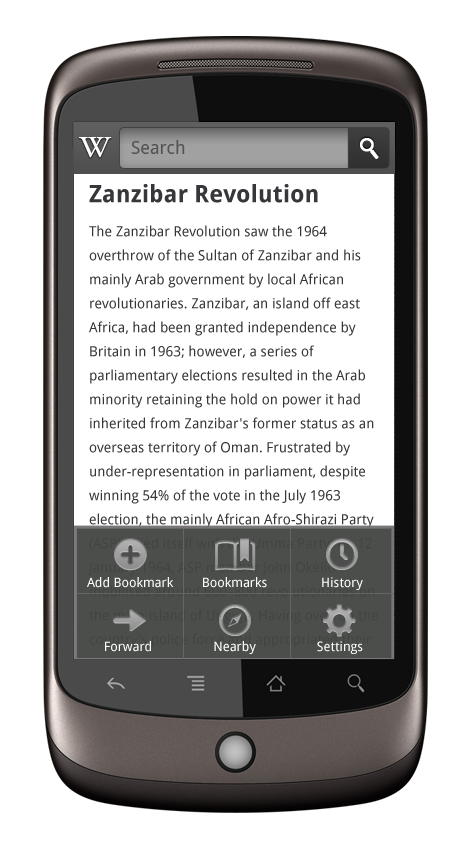
\includegraphics[width=0.4\textwidth]{wikipedia.png}
\caption{Aplikace Wikipedia na OS Android \cite{google_android_wikipedia}.}
\label{fig:WikipediaApp}
\end{figure} 

\subsection{BBC Olympics}
Pro účely letních olympijských her v Londýně v létě 2012 vznikla pro britskou veřejnoprávní televizi BBC aplikace, která umožnila uživatelům přísun čerstvých novinek z dění na sportovištích. Aplikace nabízela například živé videopřenosy ze všech sportovišť, živý textový komentář k jednotlivým sportům, sestřihy toho nejlepšího, možnost čtení nejzajímavějších článků offline a mnoho dalšího. \cite{phonegap_bbc_olympics_app}

BBC Olympics byla dostupná na třech platformách – iOS, Android a Blackberry.

\begin{figure}\centering
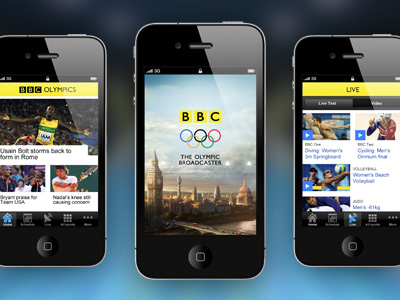
\includegraphics[width=0.5\textwidth]{bbc.jpg}
\caption{Aplikace BBC Olympics na platformě iOS \cite{dribbble_bbc_olympics}.}
\label{fig:BBCApp}
\end{figure} 

\subsection{Fruit Salad}
Fruit Salad je hra, kde se hráč snaží skládat pod sebe stejné druhy ovoce a získávat za to body. Tato hra vytvořená pomocí HTML5 je dostupná pro platformu Android.

“PhoneGap Build is a great tool for web developers who want to give App Store visibility to their HTML apps” said Fruit Salad creator, Baptiste Brunet. \cite{phonegap_fruit_salad}

\begin{figure}\centering
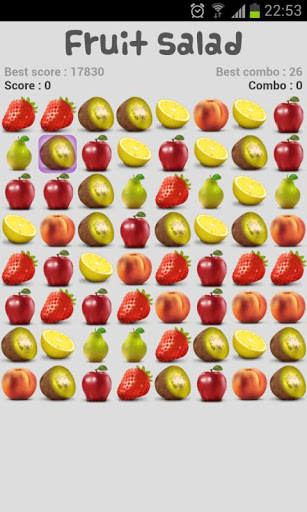
\includegraphics[width=0.4\textwidth]{fruitsalad.jpg}
\caption{Hra Fruit Salad běžící na OS Android \cite{phonegap_fruit_salad}.}
\label{fig:FruitSalad}
\end{figure} 

\section{Budoucnost}
Co očekávat od budoucích let v souvislosti s PhoneGap? Jednoznačně mnohem hlubší integraci s Adobe produkty. Ačkoliv se to již u některých produktů (Adobe DreamWeaver) stalo, od převzetí PhoneGap firmou Adobe se očekávalo v tomto ohledu mnohem více. V dalších letech tak můžeme očekávat zařazování PhoneGap do vývojářských nástrojů, které Adobe poskytuje vývojářům HTML5 aplikací.

Jak jsem již předeslal na začátku této kapitoly, cílem Phonegap je, aby PhoneGap nebyl třeba. Za tímto účelem se vývojáři PhoneGap účastní tvůrčích skupin v rámci konsorcia W3C pro vytváření nových webových standardů. Jakmile budou nové standardy vytvořeny, dá se očekávat jejich rychlá implementace do PhoneGap, jako je tomu již nyní u API pro geolokaci nebo u lokálního úložiště dat.

Dalším cílem bude větší a pohodlnější rozšiřitelnost frameworku. Pluginy by mělo být možné lépe vyhledávat a snadněji instalovat. Pokročilejší vývojáře jistě potěší i plánované vylepšování řádkového interface, kterým je možno framework ovládat z konsole. Zároveň se plánuje velká revize celého API a jeho pročištění a další sjednocení. Jedním z velkých cílů je, aby bylo přidání podpory pro nové platformy co možná nejjednodušší.

Když je řeč o nových platformách, bylo by dobré zmínit, které jsou další na řadě. Vývojáři ve svých plánech hovoří zejména o dvou – Tizen a Firefox OS. Tizen je open-source operační systém pro široké spektrum zařízení vyvíjený pod záštitou Linux Foundation. O Firefox OS jsem hovořil již v kapitole \ref{Sec:FxOS}. Jedná se o mobilní operační systém od společnosti Mozilla postavený čistě na webových technologií pomocí W3C standardů a také Mozilla WebAPI.

Vydání PhoneGap ve verzi 3.0.0 je naplánováno na červenec 2013. \cite{cordova_roadmapprojects}

% Kapitola Demo aplikace
\chapter{Demo aplikace}
	Součástí této práce jsou i tři ukázkové aplikace, které jsem vytvořil pomocí frameworku PhoneGap a slouží jako základní seznámení autora práce s frameworkem a také jako demonstrace použití základních API volání, které framework poskytuje.

\section{Twitter klient (BlueBirdGap)}
První aplikací, kterou jsem ve frameworku PhoneGap vytvořil, je jednoduchý klient pro sociální síť Twitter. Obsahuje pouze elementární funkce, kdy se může uživatel přihlásit svým uživatelským jménem a heslem, zobrazit svojí timeline a také odeslat na Twitter nový tweet. Aplikace byla původně zamýšlena jako multiplatformní, tedy tak, aby se dalo co možná největší množství kódu použít i na dalších platformách. Nakonec jí bylo z důvodu platformní závislosti pluginu ChildBrowser možné využít jen na platformě Android.

V průběhu vývoje jsem narazil na problémy zejména s implementací otevřeného protokolu OAuth, který je vyžadován k autentizaci uživatele na Twitteru. Implementace tohoto protokolu pomocí JavaScriptu není přímočará záležitost, neboť tento postup skýtá bezpečnostní rizika v podobě odhalení přenášených bezpečnostních klíčů. Nakonec jsem využil knihovny jsOAuth, která nabízí abstraktní rozhraní pro využití tohoto protokolu. K tvorbě uživatelského rozhraní jsem využil framework jQuery Mobile spolu s vlastními CSS styly.

\begin{figure}[htbp]\centering
\includegraphics[width=0.8\textwidth]{bbgap_timeline_2.png}
\caption{BlueBirdGap, zobrazení timeline}
\label{fig:BbGapTimeline}
\end{figure}

Pokud se zaměříme na unikátní vlastnosti frameworku PhoneGap, které byly v této aplikaci využity, musím na prvním místě uvést oficiální plugin ChildBrowser, který umožňuje v rámci WebView otevřít další WebView jako svého potomka. Této funkce bylo využito při identifikaci uživatele, kdy se mu otevře jako potomek další okno, kde musí ověřit své přihlašovací údaje na webové stránce Twitteru. Z dalších funkcí uvedených v API PhoneGap můžu zmínit například využití místní databáze localStorage pro uložení údajů o konkrétním uživateli.

Aplikace byla otestována v Android emulátoru na verzi systému 4.2.

\section{Foto aplikace (Orionids)}
V druhé aplikaci jsem chtěl vyzkoušet patrně nejpřitažlivější funkci frameworku PhoneGap, za kterou pokládám možnost jednoduše ovládat fotoaparát daného mobilního zařízení. Vytvořil jsem za tímto účelem jednoduchou aplikaci, jejímž účelem je fotografovat a ukládat obrázky padajících hvězd. Zároveň s vyfocením fotografie je zaznamenána i geografická poloha místa, kde byla fotografie pořízena. Aplikace umožňuje pořídit fotografii buď přímo či jí vybrat z nativní galerie. Všechny fotografie jsou v aplikaci uložené a je možno zobrazit jejich přehled a také si prohlédnout detail každé z nich.

Protože byl pro tvorbu uživatelského rozhraní použit framework jQTouch, který je závislý na jádře WebKit, funguje tato aplikace pouze na platformách Android a iOS. Pro uživatelské rozhraní jsem využil předpřipravených šablon frameworku jQTouch, které se automaticky přizpůsobí platformě, na které běží, aby více simulovaly vzhled nativních aplikací. Finální vzhled jsem upravil vlastními CSS styly. Pro zobrazení míst, kde byly fotografie pořízeny, je využito vložené Google mapy s vyznačením dotyčných poloh.

\begin{figure}\centering
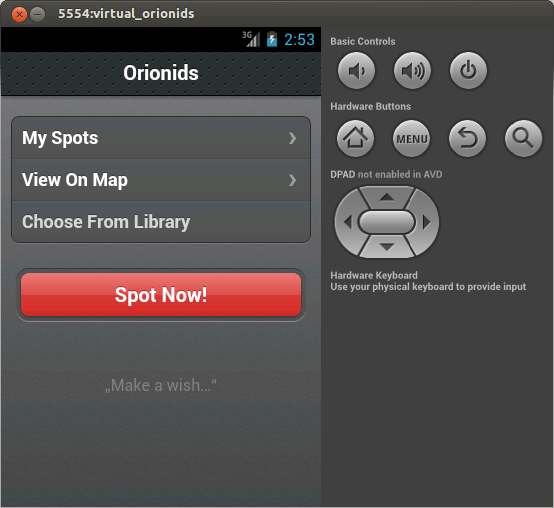
\includegraphics[width=0.8\textwidth]{orionids_home.png}
\caption{Orionids, domovská obrazovka}
\label{fig:OrionidsHome}
\end{figure}

V rámci této aplikace bylo rovněž využito několik API volání, které vývojářům nabízí framework PhoneGap. Stěžejním bylo pochopitelně využití API volání Camera, které umožňuje pořídit fotografii fotoaparátem či ji vybrat z nativní fotogalerie daného zařízení. Pro ukládání informací o pořízených fotografiích jsem využil volání Storage, které zpřístupňuje ukládání do lokální databáze dle specifikace konsorcia W3C. V neposlední řadě jsem využil volání Geolocation, které zpřístupňuje údaje o zeměpisné šířce a délce místa, kde se dané zařízení právě nachází. Na závěr musím podotknout, že používání všech API bylo velmi přímočaré a bezproblémové.

Aplikace byla otestována v Android emulátoru na verzi systému 4.2.

\section{Časovací aplikace (TimerGap)}
Poslední aplikací je jednoduchý časovač, který umožňuje uživateli spustit odpočítávání času využitelné například jako kuchyňská minutka pro odměření doby potřebné pro vylouhování čaje. Aplikace umožňuje spustit rychlé odpočítávání, uložit a pojmenovat odpočítávání pro další použití a samozřejmě vybírat a spouštět již uložené časy.

V této aplikaci jsem opět využil JavaScriptový framework jQuery Mobile, pomocí nějž jsem vytvořil uživatelské rozhraní a také využil jeho funkcí při tvorbě funkční logiky celé aplikace. Pro realizaci vlastního odpočítávání jsem využil knihovnu jQuery Countdown, která poskytuje pro jeho implementaci velmi podařené abstraktní rozhraní. Pro zajištění uživatelsky přívětivého způsobu vybírání času jsem využil plugin jQuery Mobile - Datebox.

\begin{figure}[htbp]\centering
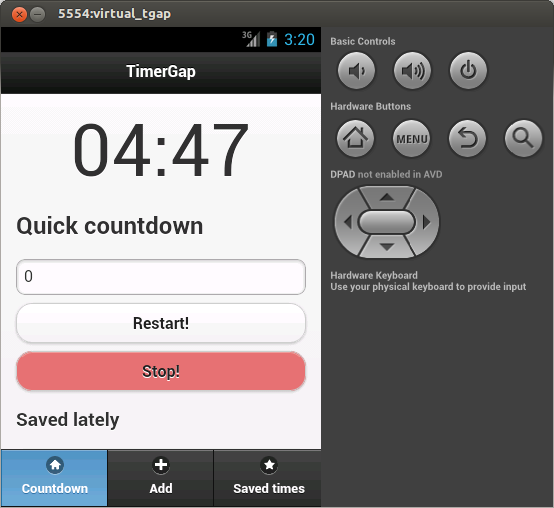
\includegraphics[width=0.8\textwidth]{tgap_odpocitavani.png}
\caption{TimerGap, proces odpočítávání}
\label{fig:TGapOdpocitavani}
\end{figure}

V této aplikaci jsem se zaměřil především na otestování notifikačních schopností frameworku PhoneGap, který nabízí několik možností jak upozornit uživatele na nějakou událost. Z rozhraní Notification  jsem využil téměř všechny nabízené možnosti: dialogy alert či confirm a v momentě vypršení odpočítávaného času také zvukové upozornění beep spolu se zavibrováním vibrate. Pro ukládání uživatelem definovaných odpočítávání jsem využil databázi localStorage.

Práce s výše zmíněnými API voláními byla poměrně bezproblémová, krom platformy Windows Phone 7, kde jsme narazil na problémy s databází localStorage, která se nad jádrem prohlížeče IE 9 chová poněkud nestandardně.
        
Aplikace byla otestována v Android emulátoru na verzi systému 4.2 a na mobilním telefonu Nokia Lumia 800 se systémem Windows Phone 7.8.

% Kapitola Hybridní vs. nativní vývoj
\chapter{Hybridní vs. nativní vývoj}
	V rámci této kapitoly se pokusím co možná nejkomplexněji srovnat hybridní a nativní přístup. Jejich porovnání se bude týkat tří klíčových oblastí z životního cyklu aplikace.

\section{Způsob vývoje}
\subsection{Náročnost vývoje}
\subsubsection{Lidské zdroje a finance}
Tyto dvě kritéria jsem spojil do jednoho, protože spolu velmi úzce souvisí. Cena vývoje aplikace totiž naprosto dominantně záleží na lidech, kteří jí vytváří. Je zřejmé, že výsledná cena závisí na mnoha faktorech, jako je například typ aplikace (jiné náklady bude třeba vynaložit na tvorbu jednoduché To-Do aplikace, jiné na vývoj 3D hry), počet platforem, na které budeme aplikaci portovat nebo aktuální situace na trhu.

Obecně se však uvádí, že vývoj hybridní aplikace je oproti nativní variantě levnější. Hlavním důvodem je, že vývojáři znalý webových technologií stojí méně než kvalifikovaní vývojáři znalí technologií nutných pro vývoj pro konkrétní platformu. Odhaduje se, že vývoj nativní aplikace stojí mezi 20 000 a 150 000 dolary \cite{mrc_native_wrong_choice}.

V obecné rovině také platí, že weboví vývojáři jsou na pracovním trhu poměrně lehce k sehnání a řada firem již takové vývojáře dokonce zaměstnává interně. V takovém případě je využití hybridního přístupu obzvláště lákavé.

Dle trendů na pracovním trhu, které sleduje server indeed.com, je poptávka po vývojářích ovládajících technologii HTML5 skutečně velká. Jedná se dokonce o nejvíce vyžadovanou dovednost ze všech pracovních nabídek, které server pravidelně analyzuje. Strmý růst poptávky po HTML5 vývojářích vidíme na grafu \ref{fig:HTML5Jobs}.

\begin{figure}\centering
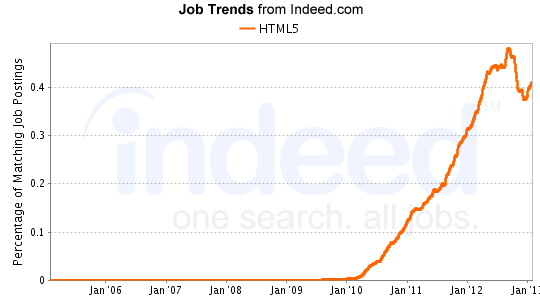
\includegraphics[width=1.0\textwidth]{jobgraph_html5.png}
\caption{Vývoj nabídek zaměstnání pro HTML5 vývojáře \cite{job_indeed}}
\label{fig:HTML5Jobs}
\end{figure}

S tímto trendem se logicky svezla i poptávka po vývojářích specializovaných na přední hybridní framework PhoneGap.

\begin{figure}\centering
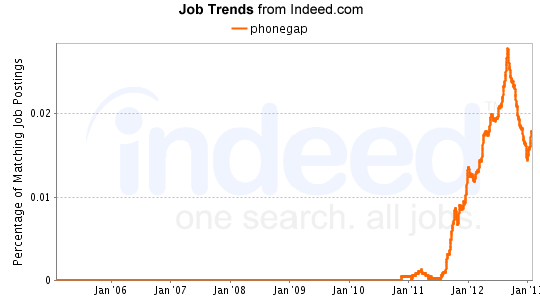
\includegraphics[width=1.0\textwidth]{jobgraph_phonegap.png}
\caption{Vývoj nabídek zaměstnání pro PhoneGap vývojáře \cite{job_indeed}}
\label{fig:PhoneGapJobs}
\end{figure}

Zajímavým ukazatelem je také průměrná mzda, kterou vývojáři s těmito schopnostmi dostávají. Průměrná mzda na pozicích, kde je vyžadována znalost HTML5 je 84 000 amerických dolarů ročně. Zaměstnanec na pozici „HTML Developer“ pak pobírá 75 000 dolarů za rok. Velice blízko těmto číslům je i průměrná mzda na pozicích, kde je jako schopnost vyžadována znalost frameworku PhoneGap, která dosahuje výše 86 000 dolarů. \cite{job_indeed}

Pokud se podíváme na nativní vývojáře, tak zjistíme, že poptávka po nich je jen nepatrně nižší.

\begin{figure}\centering
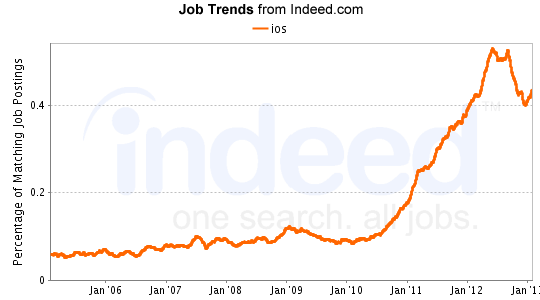
\includegraphics[width=1.0\textwidth]{jobgraph_ios.png}
\caption{Vývoj nabídek zaměstnání pro iOS vývojáře \cite{job_indeed}}
\label{fig:iOSJobs}
\end{figure}

Na datech o průměrné mzdě, která je nabízena vývojářům ovládajícím technologie pro vývoj pro iOS, je vidět, že jsou vývojáři s těmito schopnostmi nákladnější. Průměrná mzda v této oblasti dosahuje výše 89 000 dolarů za rok. Zaměstnanec na pozici „iOS Mobile Developer“ pobírá ročně 104 000 dolarů. O něco levnější je cena práce vývojáře pro platformu Android, kde si „Android Developer“ přijde na 101 000 dolarů za rok.

Dalším faktorem je také výše zmíněný počet platforem, pro které bude aplikace vyvíjena. Zatímco v případě vývoje pro jedinou platformu nemusí být rozdíl v nákladech na vývojáře markantní, v případě cílení na dvě nebo více platforem již náklady na nativní vývojáře strmě rostou. Tuto situaci názorně dokládá následující tabulka, která ukazuje odhadované náklady na vývoj multiplatformní aplikace (iOS, Android, Windows Phone) pomocí nativní i hybridní cesty.

\begin{table}\centering
	\caption[Srovnání ceny hybridního a nativního přístupu při vývoji aplikace pro 3 platformy]{Srovnání ceny hybridního a nativního přístupu při vývoji aplikace pro 3 platformy \cite{globant_hybrid}} 
	\label{tab:ComparsionCost}
		\begin{tabular}{|c|c|c|c|}\hline
			Profese	& Počet & Hodin [rok] & Roční náklady [USD]
			\tabularnewline \hline \hline
					iOS Architekt	& 1 & 2 000 & \$200 000
			\tabularnewline \hline
					iOS Developer	& 3 & 6 000 & \$300 000
			\tabularnewline \hline
				\textbf{Celkem}	& \textbf{4} & \textbf{8 000} & \textbf{\$500 000}
			\tabularnewline \hline \hline
				JavaScript Architekt	& 1 & 2 000 & \$200 000
			\tabularnewline \hline
				JavaScript Developer	& 3 & 6 000 & \$300 000
			\tabularnewline \hline
				iOS Developer	& 1 & 2 000 & \$100 000
			\tabularnewline \hline
				Android Developer	& 1 & 2 000 & \$100 000
			\tabularnewline \hline
				Windows Phone Developer	& 1 & 2 000 & \$100 000
			\tabularnewline \hline
				\textbf{Celkem}	& \textbf{7} & \textbf{14 000} & \textbf{\$800 000}
			\tabularnewline \hline \hline
				\textbf{Při vývoji pro 3 platformy} & & &
			\tabularnewline \hline
				Nativní tým & 12 & 24 000 & \$1 500 000
			\tabularnewline \hline
				Hybridní tým & 7 & 14 000 & \$800 000
			\tabularnewline \hline
				\textbf{Úspory}	& \textbf{42 \%} & \textbf{42 \%} & \textbf{47 \%}
			\tabularnewline \hline
		\end{tabular}
\end{table}

\subsubsection{Složitost}
Jednoznačně určit, který přístup je pro vývojáře složitější, je náročné. Pro každého jedince je subjektivně složité něco jiného.

Obecně lze říci, že vývoj nativních aplikací vyžaduje rozsáhlejší znalosti, než-li je tomu při vývoji pomocí webových technologií. I hybridní vývojář však musí velmi dobře rozumět JavaScriptovému frameworku, který používá. Je třeba si uvědomit, že vývoj mobilních aplikací se v mnoha ohledech výrazně liší od vývoje klasických webových stránek.

\subsection{Rychlost vývoje}
Toto kritérium je více než všechny ostatní závislé na komplexnosti vyvíjené aplikace. Velmi jednoduchá aplikace může být vyvinuta v řádu dnů až týdnů jak nativně tak hybridně. U složitější aplikace zas doba strávená jejím vývojem závisí na jiných faktorech (počet vývojářů, počet platforem apod.). Výzkum společnosti Forrester Research udává, že vývoj nativní aplikace zabere vývojovému týmu průměrně 6 měsíců \cite{mrc_native_wrong_choice}. Pokud je aplikace vyvíjena pro více platforem, je jasné, že se doba vývoje prodlouží kvůli neustálé nutnosti koordinace vývojových týmů s cílem přinést konzistentní UX napříč platformami.

Zřejmě tedy nebudeme daleko od pravdy, když řekneme, že v obecném slova smyslu je vývoj hybridních aplikací méně časově náročný než vývoj nativní. To je způsobeno zejména možností využití jedné sady zdrojových kódů pro port aplikace na různé platformy.

\subsection{Nástroje}
\subsubsection{Vývojové prostředí}
Volba správného vývojového prostředí je pro pohodlný a rychlý vývoj mobilní aplikace klíčová. Vývojáři nativních aplikací v drtivé většině používají vývojová prostředí dodávaná s SDK konkrétní platformy. Pro iOS tedy vyvíjejí v XCode, pro Android v Eclipse, pro Windows Phone ve Visual Studiu a tak podobně. Tato prostředí jim poskytují možnost správy projektů, tvorby zdrojového kódu a také nezbytné ladící nástroje. Pomocí těchto prostředí je rovněž možné odeslat hotovou aplikaci na oficiální tržiště dané platformy.

Vývojáři hybridních aplikací mají ve volbě svého vývojového prostředí zdánlivě větší svobodu. Od uvedení nástroje PhoneGap Build (viz. kapitola \ref{Sec:PhoneGapBuild}) již nejsou nuceni pro vytvoření nativních instalačních balíčků používat SDK konkrétní platformy. V zásadě nic pak vývojáři nebrání používat pro vývoj libovolné vývojové prostředí dle vlastních preferencí (například oblíbený textový editor).

\subsubsection{Testování a debugging}
V tomto případě je situace podobná jako u vývojových prostředí. Pro nativní vývojáře jsou ladící a testovací nástroje dodávány jako součást SDK. Přímo z vývojového prostředí tedy spouští svou aplikaci v emulátoru a využívají debugovací nástroje vytvořené přímo za účelem ladění mobilních aplikací pro danou platformu.

Hybridní vývojáři mají situaci obtížnější. Mohou sice také využívat nativních nástrojů z SDK, ale pouze v omezené míře, neboť tyto nejsou vhodné pro ladění aplikací napsaných webovými jazyky. Hybridní vývojáři proto nejčastěji používají kombinaci nástrojů (nativní emulátor + webový prohlížeč + Ripple + Weinre) [viz kapitola \ref{Sec:DebugaTest}]. Nativní emulátor mohou spouštět buď z vývojového prostředí určeného pro vývoj nativních aplikací (například Eclipse) nebo pomocí konsolového interface, který poskytuje například framework PhoneGap.

\subsubsection{Podpora}
Každý vývojář se v průběhu vývoje mnohokrát dostane do situace, kdy neví jak dál a potřebuje pomoci. Tuto pomoc může získat z celé řady zdrojů jako jsou například knižní příručky, placená podpora, internetové články a internetová komunitní fóra.

V této oblasti mají nativní vývojáři zatím jasně navrch, což je dáno zejména tím, že hybridní přístup je poměrně nový. Počet knih i internetových příruček zabývajících se hybridním vývojem je oproti nativnímu signifikantně nižší. Kolem vývoje nativních aplikací pro konkrétní platformu je vytvořen celý prstenec nástrojů, které mohou vývojáři používat, když potřebují pomoci. Jedná se o IRC chaty, specializované diskuzní skupiny či možnost nechat si poradit od odborníků v rámci office hours (Android). Množství zodpovězených otázek[d] na populárním komunitním diskuzním fóru stackoverflow.com vyznívá také jasně ve prospěch nativní cesty.

Hybridní vývojář má (krom oficiální dokumentace) na výběr z nízkého (ale stále rostoucího) počtu různých internetových tutoriálů, které mu pomohou v začátcích. Na trhu je také k dispozici řada knih (v angličtině) většinově zaměřených na úvod do vývoje v konkrétním hybridním frameworku (dominantně PhoneGap). Každý framework má kolem sebe také vytvořenu určitou komunitu, kde může vývojář hledat pomoc (typicky diskuzní fóra). Framework PhoneGap poskytuje i možnost placené podpory pro vývojáře. 

Lze tedy říci, že v případě hybridní cesty již existuje poměrně solidní množství materiálů pro začínající vývojáře, ale v případě komplikovanějších problémů je již vývojář odkázán na pomoc komunity kolem serverů, jako je například stackoverflow.com.

\section{Vlastní aplikace}
\subsection{Vzhled}
Ve světě mobilních aplikací není vzhled jen otázkou vkusu. Uživatelé chytrých mobilních telefonů jsou zvyklí, že aplikace běžící na jejich platformě vypadají a chovají se v určitých aspektech obdobně. Díky tomu se rychle naučí s aplikací pracovat a její používání je pro ně příjemné, protože aplikace reaguje tak, jak očekávají.

Hybridní aplikace jsou pohledem tohoto kritéria jednoznačně pozadu. Hlavním problémem je, že nevyužívají nativních UI elementů a nahrazují je pomocí CSS a JavaScriptu. Kvalifikovaný vývojář hybridních aplikací dokáže pomocí těchto technologií napodobit vzhled nativních elementů velmi věrně, nikoliv však dokonale. Méně zkušený vývojář pak často sáhne po UI elementech, které mu nabízí JavaScriptový framework, jakým je například jQuery Mobile. Díky tomu dokáže vytvořit uživatelské prostředí velmi rychle, jeho podoba je však od té nativní již vzdálenější.

S tímto problémem se potýkáme ve všech oblastech UX hybridní aplikace. Nejedná se jen o vzhled samotných elementů, ale i o přechody mezi jednotlivými obrazovkami či odezvu na uživatelské vstupy. Pokud chceme, aby většina uživatelů nepoznala, že aplikace kterou používají, je hybridní, je zapotřebí najmout skutečně kvalifikovaného CSS vývojáře.

Oproti tomu nativní aplikace plně využívají nativních UI elementů a dosahují tak přirozeného vzhledu i očekávaných reakcí uživatelského prostředí.

\subsection{Odezva}
Odezva přímo souvisí s výše zmíněným kritériem vzhledu. Když uživatel „tapne“[e] na tlačítko, očekává okamžitou odpovídající reakci. Nativní UI elementy toto zaručují, u napodobenin jež využíváme v hybridních aplikacích, je již situace složitější. V hybridních aplikacích jsme odkázáni na události, které definuje norma jazyka JavaScript nebo námi zvolený JavaScriptový framework. Hlavním problémem je, že JavaScript ve výčtu definovaných událostí příliš nepočítá s dotykovými zařízeními a tak může být odezva aplikací, jejichž uživatelské prostředí na těchto událostech závisí pomalejší, než je tomu u jejich nativních protějšků.

Dobrou ilustrací tohoto problému je událost „click“. Tato událost vznikla proto, aby dala webovým aplikacím možnost dynamicky reagovat na kliknutí myši. JavaScriptový engine rozpozná událost „click“ tak, že po stisknutí pravého tlačítka čeká 300 milisekund a kontroluje, zda je po této době tlačítko stále stisknuto. Pokud ano, nastane událost „click“. Při ovládání aplikací dotykem prstu však může chování této události způsobovat problémy. „Tapnutí“ prstem je typicky velmi krátké a pokud je aplikace připravena reagovat na událost „click“, nemusí „tapnutí“ zaznamenat a uživatel je tak nucen celou akci opakovat. Tohoto problému si byli vědomi tvůrci frameworků, jako je například jQuery Mobile, a vytvořili událost „tap“, která nemá nastaveno tak dlouhé čekání a tudíž lépe reaguje na ovládání prstem.

\subsection{Výkon}
Hledisko výkonu mobilních aplikací je zmiňováno prakticky v každém serióznějším článku zabývajícím se jejich vývojem pomocí různých přístupů. V naprosté většině z nich je slabší výkon zmiňován jako hlavní nevýhoda hybridních aplikací. Dle výzkumu společnosti Vision Mobile je právě problém s výkonem nejčastějším důvodem k zavržení hybridního přístupu \cite{visionmobile_survey}.

Obecně se udává, že hybridní přístup není vhodný pro aplikace náročné na grafiku a výkon. Důvodem výkonnostních problémů u hybridních aplikací je nativní mezivrstva a zejména pak JavaScriptový engine. Ačkoliv tyto enginy neustále zrychlují, stále se nedokáží vyrovnat rychlosti nativních interpretů.

Nadále tedy platí, že pro hry a jiné výkonnostně náročnější aplikace je nativní cesta prakticky jedinou možnou, pokud chceme uživateli dopřát příjemný zážitek z používání aplikace.

\subsection{Míra integrace s OS}
Ačkoliv je schopnost využívat nativních komponent systému udávána jako jedna z hlavních předností hybridního přístupu, je logické, že oproti nativním budou hybridní aplikace vždy o krok pozadu. Nejpopulárnější hybridní framework PhoneGap podporuje v současnosti 16 nativních API volání, což je samozřejmě řádově méně než mají k dispozici vývojáři nativních aplikací.

Jedním z hlavních důvodů, proč je pro vývojáře hybridních aplikací dostupný menší počet nativních API volání, je sama multiplatformnost hybridních frameworků. Tím, že se tyto frameworky snaží podporovat co nejširší množství mobilních platforem, jsou tím pádem nuceni podporovat pouze nejmenšího společného dělitele nativních komponent všech platforem, aby použití frameworku bylo konzistentní.

\section{Monetizace}
Při výběru technologie, kterou vývojář při tvorbě aplikace použije, hraje roli i něco, čemu říkáme obchodní model kolem dané aplikace. Pokud chce vývojář na aplikaci vydělat peníze, má několik možností, jak toho docílit:

\begin{enumerate}
	\item Aplikace bude placená a uživatel za ní zaplatí při stažení na oficiálním tržišti.
	\item Reklamy uvnitř aplikace.
	\item Nákupy uvnitř aplikace.
\end{enumerate}

Zatímco u první možnosti monetizace není mezi hybridními a nativními aplikacemi rozdíl, u zbývajících dvou již zjistíme, že hybridní aplikace na tomto poli zaostávají. Přestože existují pluginy pro reklamní sítě jako je AdMob či iAds, které tuto funkcionalitu přináší (PhoneGap), jsou vyvíjeny sporadicky a uživatelé si často stěžují na problémy. Stejná situace je i v případě nákupů uvnitř aplikace, kde vývojáři reportují nekompatibilitu s novými verzemi PhoneGap i s novými verzemi operačních systémů. Pokud chce vývojář na svých aplikacích vydělávat, měl by si použití hybridního přístupu důkladně promyslet a ověřit si, že pro jím podporovanou platformu existuje ověřené fungující řešení.

\section{Shrnutí}
Výše nastíněné srovnání je samozřejmě nutno brát s určitou rezervou. Vždy primárně záleží na typu aplikace, na jejím účelu a cílové skupině, pro kterou je určena. Silné stránky nativního přístupu jsou výkon, monetizace nebo rozsah funkcí, které můžete ve své aplikaci nabídnout. Naopak na hybridní přístup se můžete spolehnout ve chvíli, kdy vám při vývoji aplikace primárně záleží na ceně nebo multiplatformním záběru.

V tabulce \ref{tab:ComparsionHybridNative} jsem se pokusil shrnout zásadní srovnávací kritéria a každý přístup v rámci nich ohodnotit. Nativní přístup dosáhl lepšího hodnocení v 5 oblastech, hybridní přístup si připsal lepší skóre ve 3 oblastech.
\begin{table}\centering
	\caption[Porovnání hybridního a nativního přístupu v klíčových oblastech]{Porovnání hybridního a nativního přístupu v klíčových oblastech \cite{mobile_dev_nat_hybrid_graph}} 
	\label{tab:ComparsionHybridNative}
		\begin{tabular}{|c|c|c|}\hline
			Oblast	& Hybridní přístup & Nativní přístup
			\tabularnewline \hline \hline
					Multiplatformní záběr	& \textbf{5} & 1
			\tabularnewline \hline
					Bezpečnost	& 1 & \textbf{5}
			\tabularnewline \hline
				Distribuce aplikace & \textbf{5} & \textbf{5}
			\tabularnewline \hline
				Monetizace	& 1 & \textbf{5}
			\tabularnewline \hline
				Aktualizace & \textbf{5} & 1
			\tabularnewline \hline
				Cena & \textbf{5} & 1
			\tabularnewline \hline
				UX & 1 & \textbf{5}
			\tabularnewline \hline
				Výkon & 1 & \textbf{5}
			\tabularnewline \hline
				Rozsah funkcí & 1 & \textbf{5}
			\tabularnewline \hline
		\end{tabular}
\end{table}

\begin{conclusion}
	V rámci této práce jsem se snažil analyzovat problematiku multiplatformního vývoje mobilních aplikací ze všech možných úhlů. Na závěr se rozhodně nechci pouštět do vynášení obecných soudů, spíše bych rád shrnul poznatky, které jsem během studia dané problematiky načerpal a také se pokusil odhadnout, jaká budoucnost hybridní frameworky čeká.


Pro hybridní přístup je na trhu bezpochyby prostor, který se bude dle mého názoru nadále zvětšovat. Již v dnešní době máme na mobilním trhu tři nebo čtyři silné hráče, kteří jsou pro tvůrce aplikací zajímaví. V dalších letech se bude tento „long tail“ nadále zvětšovat zejména díky příchodu dalších menších hráčů. Mezi nimi si můžeme uvést například Firefox OS, jehož cílem je obsadit trh s low-endovými chytrými telefony na rozvojových trzích, dále Ubuntu Phone, který přenáší prostředí nejpopulárnější Linuxové distribuce na mobilní zařízení. Sledovat se vyplatí i projekt Tizen či znovuzrození webOS. 


Existuje tedy důvod domnívat se, že v přístích letech tu bude krom iOS, Androidu, Windows Phone a BlackBerry další silná skupina platforem s menším podílem, která však dohromady bude zabírat pro vývojáře zajímavou část trhu. Tento bobtnající „long tail“ tedy může být jedním z důvodů, proč bude hybridní přístup pro vývojáře stále atraktivnější. Je zajímavé si všimnout, že tito menší hráči jako Firefox OS nebo Ubuntu Phone přímo počítají s webovými/hybridními aplikacemi jakožto plnohodnotným přístupem k vývoji aplikací.


Na druhou misku vah je však třeba položit aktuální nezralost hybridních frameworků, která brání masovému přijetí tohoto přístupu mezi vývojáři. Hlavním problémem je především výkon. I na poměrně jednoduchých aplikacích lze poznat, že byly vyvinuty hybridní cestou. Především absence nativních UI elementů a nedostatečná rychlost javascriptových enginů jsou hlavními důvody, proč hybridní aplikace výkonově zaostávají. Musím na tomto místě opět připomenout výzkum společnosti Vision Mobile, kde se 29 \% vývojářů vyjádřilo, že právě problém s výkonem byl hlavním důvodem k opuštění hybridní cesty. Pro překonání tohoto problému je třeba mít hluboké znalosti CSS a javascriptových frameworků, což ovšem může výrazně zvýšit náklady na tvorbu aplikace.


Bude zajímavé sledovat, jak se s narůstajícím podílem hybridních aplikací vyrovnají tvůrci současných lídrů na trhu mobilních platforem. Jejich zájmem totiž rozhodně není, aby se aplikace tvořily jednotně pro všechny platformy. Pokud vývojář napíše aplikaci exkluzivně pro jednu platformu, dává jí to zajímavou výhodu před konkurencí. Dobrým příkladem je například populární Instagram, který měl po dlouhou dobu aplikaci pouze pro systém iOS. 


Tvůrci těchto platforem přitom mají nad hybridními aplikacemi velkou moc. Nemusí jim povolit přístup na svá oficiální tržiště či jim mohou komplikovat život pomocí úprav webového runtime, který je pro většinu hybridních frameworků životně důležitý. Prvním náznakem takového omezování je přístup společnosti Apple, která poskytuje vývojářům webový runtime s pomalejším javascriptovým enginem, než jaký sama využívá ve svém vlastním mobilním prohlížeči. Pravděpodobně tedy můžeme očekávat další podobné překážky, které budou hybridním frameworkům kladeny do cesty, v rámci snahy o zachování důležité konkurenční výhody.


Velký potenciál pro hybridní přístup vidím v segmentu firemních aplikací. Takzvaný BYOD (Bring Your Own Device) přístup začíná nabývat na síle i u nás a otvírá tím hybridním aplikacím dveře dokořán. U firemních aplikací, které jsou využívány primárně zaměstnanci k přístupu k datům z informačních systémů, totiž příliš nezáleží na vzhledu ani na špičkovém výkonu mobilní aplikace. Důležitější je multiplatformní pokrytí a nízké náklady, tedy kritéria, v nichž hybridní přístup vyniká. Není náhodou, že Demokratická strana ve Spojených státech využívala hybridní aplikace ke koordinaci dobrovolníků pracujících na kampani Baracka Obamy. Důvod je zřejmý. Každý dobrovolník si mohl takovou aplikaci nainstalovat na svůj chytrý telefon nehledě na to, jaký operační systém používá. A stranu to přišlo na minimální náklady.


Budoucnost hybridních frameworků tedy skýtá mnoho příležitostí, které mohou posunout tento přístup ještě více do centra zájmu vývojářů mobilních aplikací. K tomu, aby se hybridní aplikace mohly směle poměřovat s těmi nativnímí, musí však urazit ještě velmi dlouhou cestu. V příštích letech se jako uživatelé budeme jistě nadále setkávat především s nativními aplikacemi. To platí zejména pro herní tituly a další výkonově náročnější aplikace. Dynamický vývoj HTML5, nárust „long tailu“ na trhu s mobilními platformami a rozšířování BYOD přístupu ve firmách však dává hybridnímu přístupu příležitost vychytat mnohé nedostatky a stát se v budoucnu plnohodnotnou cestou, kterou budou vývojáři vyvíjet mobilní aplikace.
\end{conclusion}

\bibliographystyle{csn690}
\bibliography{Mobilni_zarizeni_a_aplikace,Mobilni_platformy_technicky,Multiplatformni_vyvoj,Hybridni_frameworky,PhoneGap,Hybridni_vs_nativni_vyvoj}
\nocite{*}

\appendix

\chapter{Seznam použitých zkratek}
% \printglossaries
\begin{description}
	\item[GUI] Graphical user interface
	\item[XML] Extensible markup language
\end{description}

% TODO
% 1. Označkovat text
% 2. Doplnit obrázky
% 3. Doplnit reference
% 4. Vytvořit seznam literatury
% 5. Doplnit citace


% % % % % % % % % % % % % % % % % % % % % % % % % % % % 
% % Tuto kapitolu z výsledné práce ODSTRAŇTE.
% % % % % % % % % % % % % % % % % % % % % % % % % % % % 
% 
% \chapter{Návod k~použití této šablony}
% 
% Tento dokument slouží jako základ pro napsání závěrečné práce na Fakultě informačních technologií ČVUT v~Praze.
% 
% \section{Výběr základu}
% 
% Vyberte si šablonu podle druhu práce (bakalářská, diplomová), jazyka (čeština, angličtina) a kódování (ASCII, \mbox{UTF-8}, \mbox{ISO-8859-2} neboli latin2 a nebo \mbox{Windows-1250}). 
% 
% V~české variantě naleznete šablony v~souborech pojmenovaných ve formátu práce\_kódování.tex. Typ může být:
% \begin{description}
% 	\item[BP] bakalářská práce,
% 	\item[DP] diplomová (magisterská) práce.
% \end{description}
% Kódování, ve kterém chcete psát, může být:
% \begin{description}
% 	\item[UTF-8] kódování Unicode,
% 	\item[ISO-8859-2] latin2,
% 	\item[Windows-1250] znaková sada 1250 Windows.
% \end{description}
% V~případě nejistoty ohledně kódování doporučujeme následující postup:
% \begin{enumerate}
% 	\item Otevřete šablony pro kódování UTF-8 v~editoru prostého textu, který chcete pro psaní práce použít -- pokud můžete texty s~diakritikou normálně přečíst, použijte tuto šablonu.
% 	\item V~opačném případě postupujte dále podle toho, jaký operační systém používáte:
% 	\begin{itemize}
% 		\item v~případě Windows použijte šablonu pro kódování \mbox{Windows-1250},
% 		\item jinak zkuste použít šablonu pro kódování \mbox{ISO-8859-2}.
% 	\end{itemize}
% \end{enumerate}
% 
% 
% V~anglické variantě jsou šablony pojmenované podle typu práce, možnosti jsou:
% \begin{description}
% 	\item[bachelors] bakalářská práce,
% 	\item[masters] diplomová (magisterská) práce.
% \end{description}
% 
% \section{Použití šablony}
% 
% Šablona je určena pro zpracování systémem \LaTeXe{}. Text je možné psát v~textovém editoru jako prostý text, lze však také využít specializovaný editor pro \LaTeX{}, např. Kile.
% 
% Pro získání tisknutelného výstupu z~takto vytvořeného souboru použijte příkaz \verb|pdflatex|, kterému předáte cestu k~souboru jako parametr. Vhodný editor pro \LaTeX{} toto udělá za Vás. \verb|pdfcslatex| ani \verb|cslatex| \emph{nebudou} s~těmito šablonami fungovat.
% 
% Více informací o~použití systému \LaTeX{} najdete např. v~\cite{wikilatex}.
% 
% \subsection{Typografie}
% 
% Při psaní dodržujte typografické konvence zvoleného jazyka. České \uv{uvozovky} zapisujte použitím příkazu \verb|\uv|, kterému v~parametru předáte text, jenž má být v~uvozovkách. Anglické otevírací uvozovky se v~\LaTeX{}u zadávají jako dva zpětné apostrofy, uzavírací uvozovky jako dva apostrofy. Často chybně uváděný symbol "{} (palce) nemá s~uvozovkami nic společného.
% 
% Dále je třeba zabránit zalomení řádky mezi některými slovy, v~češtině např. za jednopísmennými předložkami a spojkami (vyjma \uv{a}). To docílíte vložením pružné nezalomitelné mezery -- znakem \texttt{\textasciitilde}. V~tomto případě to není třeba dělat ručně, lze použít program \verb|vlna|.
% 
% Více o~typografii viz \cite{kobltypo}.
% 
% \subsection{Obrázky}
% 
% Pro umožnění vkládání obrázků je vhodné použít balíček \verb|graphicx|, samotné vložení se provede příkazem \verb|\includegraphics|. Takto je možné vkládat obrázky ve formátu PDF, PNG a JPEG jestliže používáte pdf\LaTeX{} nebo ve formátu EPS jestliže používáte \LaTeX{}. Doporučujeme preferovat vektorové obrázky před rastrovými (vyjma fotografií).
% 
% \subsubsection{Získání vhodného formátu}
% 
% Pro získání vektorových formátů PDF nebo EPS z~jiných lze použít některý z~vektorových grafických editorů. Pro převod rastrového obrázku na vektorový lze použít rasterizaci, kterou mnohé editory zvládají (např. Inkscape). Pro konverze lze použít též nástroje pro dávkové zpracování běžně dodávané s~\LaTeX{}em, např. \verb|epstopdf|.
% 
% \subsubsection{Plovoucí prostředí}
% 
% Příkazem \verb|\includegraphics| lze obrázky vkládat přímo, doporučujeme však použít plovoucí prostředí, konkrétně \verb|figure|. Například obrázek \ref{fig:float} byl vložen tímto způsobem. Vůbec přitom nevadí, když je obrázek umístěn jinde, než bylo původně zamýšleno -- je tomu tak hlavně kvůli dodržení typografických konvencí. Namísto vynucování konkrétní pozice obrázku doporučujeme používat odkazování z~textu (dvojice příkazů \verb|\label| a \verb|\ref|).
% 
% \begin{figure}\centering
% 	
\includegraphics[width=0.5\textwidth, angle=30]{cvut-logo-bw}
% 	\caption[Příklad obrázku]{Ukázkový obrázek v~plovoucím prostředí}\label{fig:float}
% \end{figure}
% 
% \subsubsection{Verze obrázků}
% 
% % Gnuplot BW i barevně
% Může se hodit mít více verzí stejného obrázku, např. pro barevný či černobílý tisk a nebo pro prezentaci. S~pomocí některých nástrojů na generování grafiky je to snadné.
% 
% Máte-li například graf vytvořený v programu Gnuplot, můžete jeho černobílou variantu (viz obr. \ref{fig:gnuplot-bw}) vytvořit parametrem \verb|monochrome dashed| příkazu \verb|set term|. Barevnou variantu (viz obr. \ref{fig:gnuplot-col}) vhodnou na prezentace lze vytvořit parametrem \verb|colour solid|.
% 
% \begin{figure}\centering
% 	\includegraphics{gnuplot-bw}
% 	\caption{Černobílá varianta obrázku generovaného programem Gnuplot}\label{fig:gnuplot-bw}
% \end{figure}
% 
% \begin{figure}\centering
% 	\includegraphics{gnuplot-col}
% 	\caption{Barevná varianta obrázku generovaného programem Gnuplot}\label{fig:gnuplot-col}
% \end{figure}
% 
% 
% \subsection{Tabulky}
% 
% Tabulky lze zadávat různě, např. v~prostředí \verb|tabular|, avšak pro jejich vkládání platí to samé, co pro obrázky -- použijte plovoucí prostředí, v~tomto případě \verb|table|. Například tabulka \ref{tab:matematika} byla vložena tímto způsobem.
% 
% \begin{table}\centering
% 	\caption[Příklad tabulky]{Zadávání matematiky}\label{tab:matematika}
% 	\begin{tabular}{|l|l|c|c|}\hline
% 		Typ		& Prostředí		& \LaTeX{}ovská zkratka	& \TeX{}ovská zkratka	\tabularnewline \hline \hline
% 		Text		& \verb|math|		& \verb|\(...\)|	& \verb|$...$|		\tabularnewline \hline
% 		Displayed	& \verb|displaymath|	& \verb|\[...\]|	& \verb|$$...$$|	\tabularnewline \hline
% 	\end{tabular}
% \end{table}
% 
% % % % % % % % % % % % % % % % % % % % % % % % % % % % 

\chapter{Obsah přiloženého CD}

%upravte podle skutecnosti

\begin{figure}
	\dirtree{%
		.1 readme.txt\DTcomment{stručný popis obsahu CD}.
		.1 exe\DTcomment{adresář se spustitelnou formou implementace}.
		.1 src.
		.2 impl\DTcomment{zdrojové kódy implementace}.
		.2 thesis\DTcomment{zdrojová forma práce ve formátu \LaTeX{}}.
		.1 text\DTcomment{text práce}.
		.2 thesis.pdf\DTcomment{text práce ve formátu PDF}.
		.2 thesis.ps\DTcomment{text práce ve formátu PS}.
	}
\end{figure}

\end{document}
